\PassOptionsToPackage{usenames}{xcolor}
\PassOptionsToPackage{dvipsnames}{xcolor}
\documentclass[11pt,a4paper,twoside,final,titlepage,openright]{book}%
\usepackage{beamerarticle}

\usepackage[utf8]{inputenc}
\usepackage[T1]{fontenc}
\usepackage[spanish]{babel}

\usepackage{listings}
\usepackage{palatino}
\usepackage{lmodern}

%\renewcommand*\rmdefault{lmr}
%\renewcommand*\ttdefault{ppl}

\usepackage{url}
\usepackage{multicol}

\usepackage{tikz}
\usetikzlibrary{positioning}
\usetikzlibrary{arrows}
\usetikzlibrary{mindmap}

\usepackage{pgfplots}
\pgfplotsset{compat=1.5}

\usepackage{ccicons}

\tikzset{
  invisible/.style={opacity=0},
  visible on/.style={alt=#1{}{invisible}},
  alt/.code args={<#1>#2#3}{%
    \alt<#1>{\pgfkeysalso{#2}}{\pgfkeysalso{#3}} % \pgfkeysalso doesn't change the path
  },
}



\usepackage[a4paper,left=2cm,right=2cm,top=2.5cm,bottom=4cm]{geometry}
\usepackage[colorlinks=true,linkcolor=blue,citecolor=blue,urlcolor=blue,plainpages=false,bookmarksnumbered=true,pdfpagemode=UseOutlines]{hyperref}


\usepackage[nottoc]{tocbibind}

%\usepackage[fixlanguage]{babelbib}


\usepackage{graphicx}
\usepackage{xcolor}
\usepackage{tikz}
\usetikzlibrary{arrows,positioning} 

\newcommand{\textgood}[1]{%
{\color{blue!60!black}\textbf{#1}}%
}

\newcommand{\textbad}[1]{%
{\color{red!80!black}\textbf{#1}}%
}

\newcommand{\textmark}[1]{%
{\color{orange!70!black}\textbf{#1}}%
}

\newcommand{\textenum}[1]{%
{\color{blue!60!black}\textbf{#1}}%
}

\newcommand{\textemph}[1]{%
{\color{green!40!black}\textbf{#1}}%
}

\newcommand{\versionid}{2021.1}
\newcommand{\versiondate}{Abril de 2021}

\newcommand{\coursetitle}{Introducción a la programación en C++}
\newcommand{\moduleintro}{El lenguaje C++}
\newcommand{\modulehello}{Un primer programa}
\newcommand{\modulevalues}{Objetos, valores y tipos}
\newcommand{\modulevector}{Vector}
\newcommand{\moduleerrores}{Gestión de errores}
\newcommand{\modulefunciones}{Funciones y paso de parámetros}
\newcommand{\modulealcance}{Alcance, organización y parámetros}
\newcommand{\moduleclases}{Tipos definidos por el usuario}
\newcommand{\moduleiostream}{Flujos de entrada/salida}
\newcommand{\modulememdin}{Memoria dinámica}


\newtheorem{ejer}{Ejercicio}

\usepackage{url}

\usepackage{pdfpages}

\usepackage{todonotes}

%Package fancyhdr
\usepackage{fancyhdr}
\setlength{\headheight}{1.7cm}%{13.6pt}
\pagestyle{fancyplain}
\fancyhf{}
\lhead{
\includegraphics[height=1.25cm]{logos/uc3m.png}}
\chead{}
\rhead{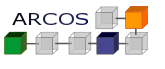
\includegraphics[height=1.25cm]{logos/arcos.png}}
\rfoot{\begin{tabular}{r}\coursetitle\\Versión \versionid\end{tabular}}
\cfoot{\begin{tabular}{c}{\thepage}\\{}\end{tabular}}
\lfoot{
\begin{tabular}{l}
\textbf{\ccbysa} -- CC BY-SA 4.0\\J. Daniel Garcia -- ARCOS@UC3M
\end{tabular}
}
\renewcommand{\headrulewidth}{0.5pt} % remove lines as well
\renewcommand{\footrulewidth}{0.5pt}
\renewcommand{\plainheadrulewidth}{0.5pt}
\renewcommand{\plainfootrulewidth}{0.5pt}

\renewcommand{\topfraction}{0.9}
\renewcommand{\textfraction}{0.1}
\renewcommand{\floatpagefraction}{0.9}

\usepackage{palatino}
\usepackage{lmodern}

\renewcommand*\rmdefault{lmr}
\renewcommand*\ttdefault{ppl}

\makeindex

\begin{document}

\mode<article>{
\lstset{
  language=C++,
  belowcaptionskip=1\baselineskip,
  breaklines=true,
  xleftmargin=\parindent,
  showstringspaces=false,
  basicstyle=\small,
  keywordstyle=\bfseries\color{green!40!black},
  commentstyle=\itshape\color{purple!40!black},
  identifierstyle=\color{blue},
  stringstyle=\color{brown},
  columns=fullflexible,
  inputencoding=utf8,
  extendedchars=true,
  morekeywords=[1]{_Pragma,constexpr,nullptr,alignof,alignas,decltype,override,final,noexcept,deprecated,thread_local,co_await,co_return,co_yield,fallthrough},
  literate=%
    {¿}{{?`}}{1}
    {¡}{{!`}}{1}
    {á}{{\'a}}{1}
    {é}{{\'e}}{1}
    {í}{{\'i}}{1}
    {ó}{{\'o}}{1}
    {ú}{{\'u}}{1}
    {ñ}{{\~n}}{1}
}
}

\mode<presentation>{
\lstset{
  language=C++,
  belowcaptionskip=1\baselineskip,
  breaklines=true,
  xleftmargin=\parindent,
  showstringspaces=false,
  basicstyle=\scriptsize,
  keywordstyle=\bfseries\color{green!40!black},
  commentstyle=\itshape\color{purple!40!black},
  identifierstyle=\color{blue},
  stringstyle=\color{orange},
  directivestyle=\bfseries\color{green!40!black},
  columns=fullflexible,
  inputencoding=utf8,
  extendedchars=true,
  morekeywords=[1]{_Pragma,constexpr,nullptr,alignof,alignas,decltype,override,final,noexcept,deprecated,thread_local,co_await,co_return,co_yield,fallthrough},
  literate=%
    {¿}{{?`}}{1}
    {¡}{{!`}}{1}
    {á}{{\'a}}{1}
    {é}{{\'e}}{1}
    {í}{{\'i}}{1}
    {ó}{{\'o}}{1}
    {ú}{{\'u}}{1}
    {ñ}{{\~n}}{1}
}
}

\newcommand{\cppkey}[1]{%
{\color{green!40!black}\textbf{#1}}%
}

\newcommand{\cppid}[1]{%
{\color{blue}\textbf{#1}}%
}

\newcommand{\cppstr}[1]{%
{\color{orange}\textbf{#1}}%
}


\lstdefinestyle{terminal}{
  language=bash,
  basicstyle=\scriptsize\ttfamily,
  numbersep=3pt,
  frame=tb,
  columns=fullflexible,
  backgroundcolor=\color{yellow!20},
}



\frontmatter

\pagestyle{empty}
\begin{titlepage}
\tikz[remember picture,overlay] \draw [fill,Blue] (current page.north west) rectangle +(0.2\paperwidth,-\paperheight);
\begin{flushright}

\includegraphics[width=5cm]{logos/uc3m.png}
\\
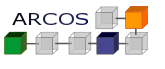
\includegraphics[width=5cm]{logos/arcos.png}
\end{flushright}

\vfill

\begin{tabular}{p{3cm}l}
&
\LARGE{Material de curso}
\\

&\\

&
\LARGE{\coursetitle}
\\

&\\

&
Version: \versionid
\\

&
\versiondate
\\

\end{tabular}
\vfill
\begin{tabular}{p{3cm}l}
&José Daniel García Sánchez\\
&Departamento de Informática\\
&Grupo ARCOS\\
&Universidad Carlos III de Madrid\\
&Av. Universidad, 30\\
&28911 Leganés, Madrid\\
&\url{josedaniel.garcia@uc3m.es}\\
\end{tabular}
\vspace{1cm}
\\
\begin{tabular}{p{3cm}l}
&
%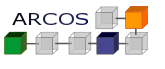
\includegraphics[width=5cm]{logos/arcos.png}
%
\includegraphics[width=8cm]{logos/logo-uc3m.jpg}
\\
\end{tabular}
\end{titlepage}

\pagestyle{fancyplain}
\chapter*{Atribución-CompartirIgual 4.0 Internacional (CC BY-SA 4.0)}

Este es un resumen legible por humanos (y no un sustituto) de la
(código legal disponible en
\url{https://creativecommons.org/licenses/by-sa/4.0/legalcode}
).

\section*{Usted es libre de:}

\begin{itemize}

\item \textbf{Compartir} --
copiar y redistribuir el material en cualquier medio o formato.

\item \textbf{Adaptar} -- 
remezclar, transformar y construir a partir del material
para cualquier propósito, incluso comercialmente.

\end{itemize}

La licenciante no puede revocar estas libertades en tanto usted siga los
términos de la licencia.

\section*{Bajo los siguientes términos:}

\begin{itemize}

\item \ccAttribution \quad \textbf{Atribución} --
Usted debe dar crédito de manera adecuada, brindar un enlace a la licencia, e
indicar si se han realizado cambios. Puede hacerlo en cualquier forma
razonable, pero no de forma tal que sugiera que usted o su uso tienen el apoyo
de la licenciante. 

\item \ccShareAlike \quad \textbf{CompartirIgual} --
Si remezcla, transforma o crea a partir del material, debe distribuir su
contribución bajo la lamisma licencia del original. 

\item \textbf{No hay restricciones adicionales} -- 
No puede aplicar términos legales ni medidas tecnológicas que restrinjan
legalmente a otras a hacer cualquier uso permitido por la licencia. 

\end{itemize}

\section*{Avisos:}

No tiene que cumplir con la licencia para elementos del materiale en el dominio
público o cuando su uso esté permitido por una excepción o limitación
aplicable.

No se dan garantías. La licencia podría no darle todos los permisos que
necesita para el uso que tenga previsto. Por ejemplo, otros derechos como
publicidad, privacidad, o derechos morales pueden limitar la forma en que
utilice el material.


\cleardoublepage
\chapter*{Presentación}

Bienvenidos


\section*{Structure}

Los contenidos de este curso se estructuran de la siguiente forma:

\begin{enumerate}

\item Introducción a C++.
\item \ldots

\end{enumerate}

\cleardoublepage
\chapter*{Agradecimientos}

En primer lugar, me gustaría dar las gracias a Bjarne Stroustrup
por darnos el lenguaje de programación C++.

También me gustaría expresar mi gratitud a todos los miembreos del
grupo de trabajo ISO/IEC JTC1/SC22/WG21, que han trabajado durante
décadas para mejorar y actualizar el lenguaje.
La discusión con muchos de ellos sobre diversos aspectos específicos
del lenguaje y de la biblioteca estándar han sido para mi de gran utilidad.

Así mismo, me gustaría agradecer de forma especial a todos aquellos
que han proporcionado realimentación sobre versiones previas de este 
material.



\cleardoublepage
\tableofcontents
\todototoc
\listoftodos

\mainmatter

\pagestyle{fancyplain}
\mode<article>{\chapter{\moduleintro}}

\section{El lenguaje C++}

\begin{frame}{¿Qué es C++?}
\mode<presentation>{

\begin{center}
\begin{tikzpicture}[small mindmap,
    concept color=blue,
    level 1 concept/.append style={font=\tiny,level distance=2.0cm},
    level 2 concept/.append style={font=\tiny,level distance=1.5cm},
    level 3 concept/.append style={font=\tiny},
    every node/.append style={scale=0.8},
    text=white,
    ]
  \node [concept, font=\small] {C++}
    child [grow=25, visible on=<1->] {node[concept] {Es C con ...}}
    child [grow=340, visible on=<2->] {node[concept, visible on=<2->] {Demasiado \ldots}
      child [grow=40, visible on=<3->]{node[concept] {difícil}}
      child [grow=0, visible on=<4->]{node[concept] {bajo nivel}}
      child [grow=320, visible on=<5->]{node[concept] {alto nivel}}
    }
    child [grow=90,visible on=<6->] {node[concept] {Programación}
      child [grow=20,visible on=<7->]{node[concept] {Orientada a objetos}
        child [grow=30]{node[concept] {Clases}}
        child [grow=330]{node[concept] {Jerarquías de clases}}
      }
      child [grow=150,visible on=<8->] {node[concept] {Genérica}
        child [grow=140] {node[concept] {Metapro\-gramción}}
      }
      child [grow=200, visible on=<9->] {node[concept] {Funcional}
        child [grow=150] {node[concept] {Lambdas}}
        child [grow=210] {node[concept] {Genéricos}}
      }
      child [grow=90,visible on=<10->]{node[concept] {Multi\-paradigma}}
    }
    child [grow=210, level distance=2.25cm,visible on=<11->] {node[concept] {Problemas}
      child [grow=200, visible on=<12->] {node[concept] {Buffer overflow}}
      child [grow=150,visible on=<12->] {node[concept] {Goteos de memoria}}
    }
  ;
\end{tikzpicture}
\end{center}

}
\mode<article>{

\begin{itemize}
  \item C++ es:
    \begin{itemize}
      \item (C89, C99, C11, C17).
      \item Demasiado:
        \begin{itemize}
          \item Demasiado grande.
          \item Demasiado alto nivel.
          \item Demasiado bajo nivel.
        \end{itemize}
      \item Programación:
        \begin{itemize}
          \item Orientada a objetos: clases, jerarquías, polimorfismo dinámico.
          \item Genérica: Plantillas.
          \item Funcional: Funcional: Lambdas, metaprogramación.
          \item Multiparadigma.
        \end{itemize} 
      \item Problemas:
        \begin{itemize}
          \item Goteos de memoria.
          \item \emph{Buffer overflow}.
        \end{itemize}
    \end{itemize}
\end{itemize}
}
\end{frame}

\begin{frame}[t]{Ventajas de C++ (perspectiva de negocio)}
\begin{itemize}
  \item Enorme base de usuarios y código existente.
    \begin{itemize}
      \item Rico ecosistema de proveedores de herramientas y servicios.
    \end{itemize}
  \item Permite ofrecer interfaces simplificadas a componentes software.
  \item Sobrecarga de operadores simplifica curvas de aprendizaje.
  \item Reduce la tensión entre seguridad y velocidad.
  \item Facilita la reutilización de código mediante polimorfismo estático y dinámico.
\end{itemize}
\end{frame}

\begin{frame}{¿De donde viene?}
\begin{itemize}
  \item \pause Influencias de alto nivel.
    \begin{itemize}
      \item Lenguajes de abstracción de propósito general.
        \begin{itemize}
          \item Simula.
        \end{itemize}
      \item Lenguajes de abstración de dominio específico.
        \begin{itemize}
          \item FORTRAN, COBOL.
        \end{itemize}
    \end{itemize}
  \item \pause Influencias de bajo nivel.
    \begin{itemize}
      \item Correspondencia directa con el hardware.
        \begin{itemize}
          \item Ensamblador.
        \end{itemize}
      \item Abstracción mínima del hardware.
        \begin{itemize}
          \item BCPL.
          \item C.
        \end{itemize}
    \end{itemize}
  \item \pause Influencias sobre otros lenguajes.
    \begin{itemize}
      \item Java.
      \item C\#.
      \item C (C11).
    \end{itemize}
\end{itemize}
\end{frame}

\begin{frame}{Evolución}
\vspace{-0.5em}
\begin{itemize}
  \item Serie de normas ISO/IEC 14882 (1998, 2011, 2014, 2017, 2020, \ldots).
  \mode<presentation>{\vfill\pause}
  \item \textmark{``Un lenguaje de programación de abstracciones ligeras''} (B. Stroustroup).
  \mode<presentation>{\vfill\pause}
  \item Evolución de C++.
    \begin{itemize}
      \item Tiene muchos elementos de compatibilidad.
        \begin{itemize}
          \item La raíz histórica de algunos llega hasta 1972.
        \end{itemize}
      \item Evolucionar un lenguaje con miles de millones de línea de código es
      distinto que diseñar un nuevo lenguaje de programación.
    \end{itemize}
  \mode<presentation>{\vfill\pause}
  \item Si alguien dice que tiene un lenguaje de programación perfecto:
    \begin{itemize}
      \item Es na\"{i}ve.
      \item Es un vendedor.
    \end{itemize}
\end{itemize}
\end{frame}

\begin{frame}[t]{Normalización}
\begin{itemize}
  \item 1998: C++98 $\rightarrow$ ISO/IEC 14882:1998
  \item 2003: C++03 $\rightarrow$ ISO/IEC 14882:2003.
    \begin{itemize}
      \item Technical Corrigendum
    \end{itemize}
  \item 2005: C++ TR1 $\rightarrow$ ISO/IEC TR 19768.
    \begin{itemize}
      \item C++ Library Extensions
    \end{itemize}
  \item 2011: C++11 $\rightarrow$ ISO/IEC 14882:2011.
  \item 2014: C++14 $\rightarrow$ ISO/IEC 14882:2014. 
  \item 2017: ISO/IEC 14882:2017.
  \item 2020: ISO/IEC 14882:2020.
  \item 2023: \textbad{Probablemente} ISO/IEC 14882:2023.
\end{itemize}
\end{frame}

\mode<presentation>{
\begin{frame}{C++ timeline}
\centering
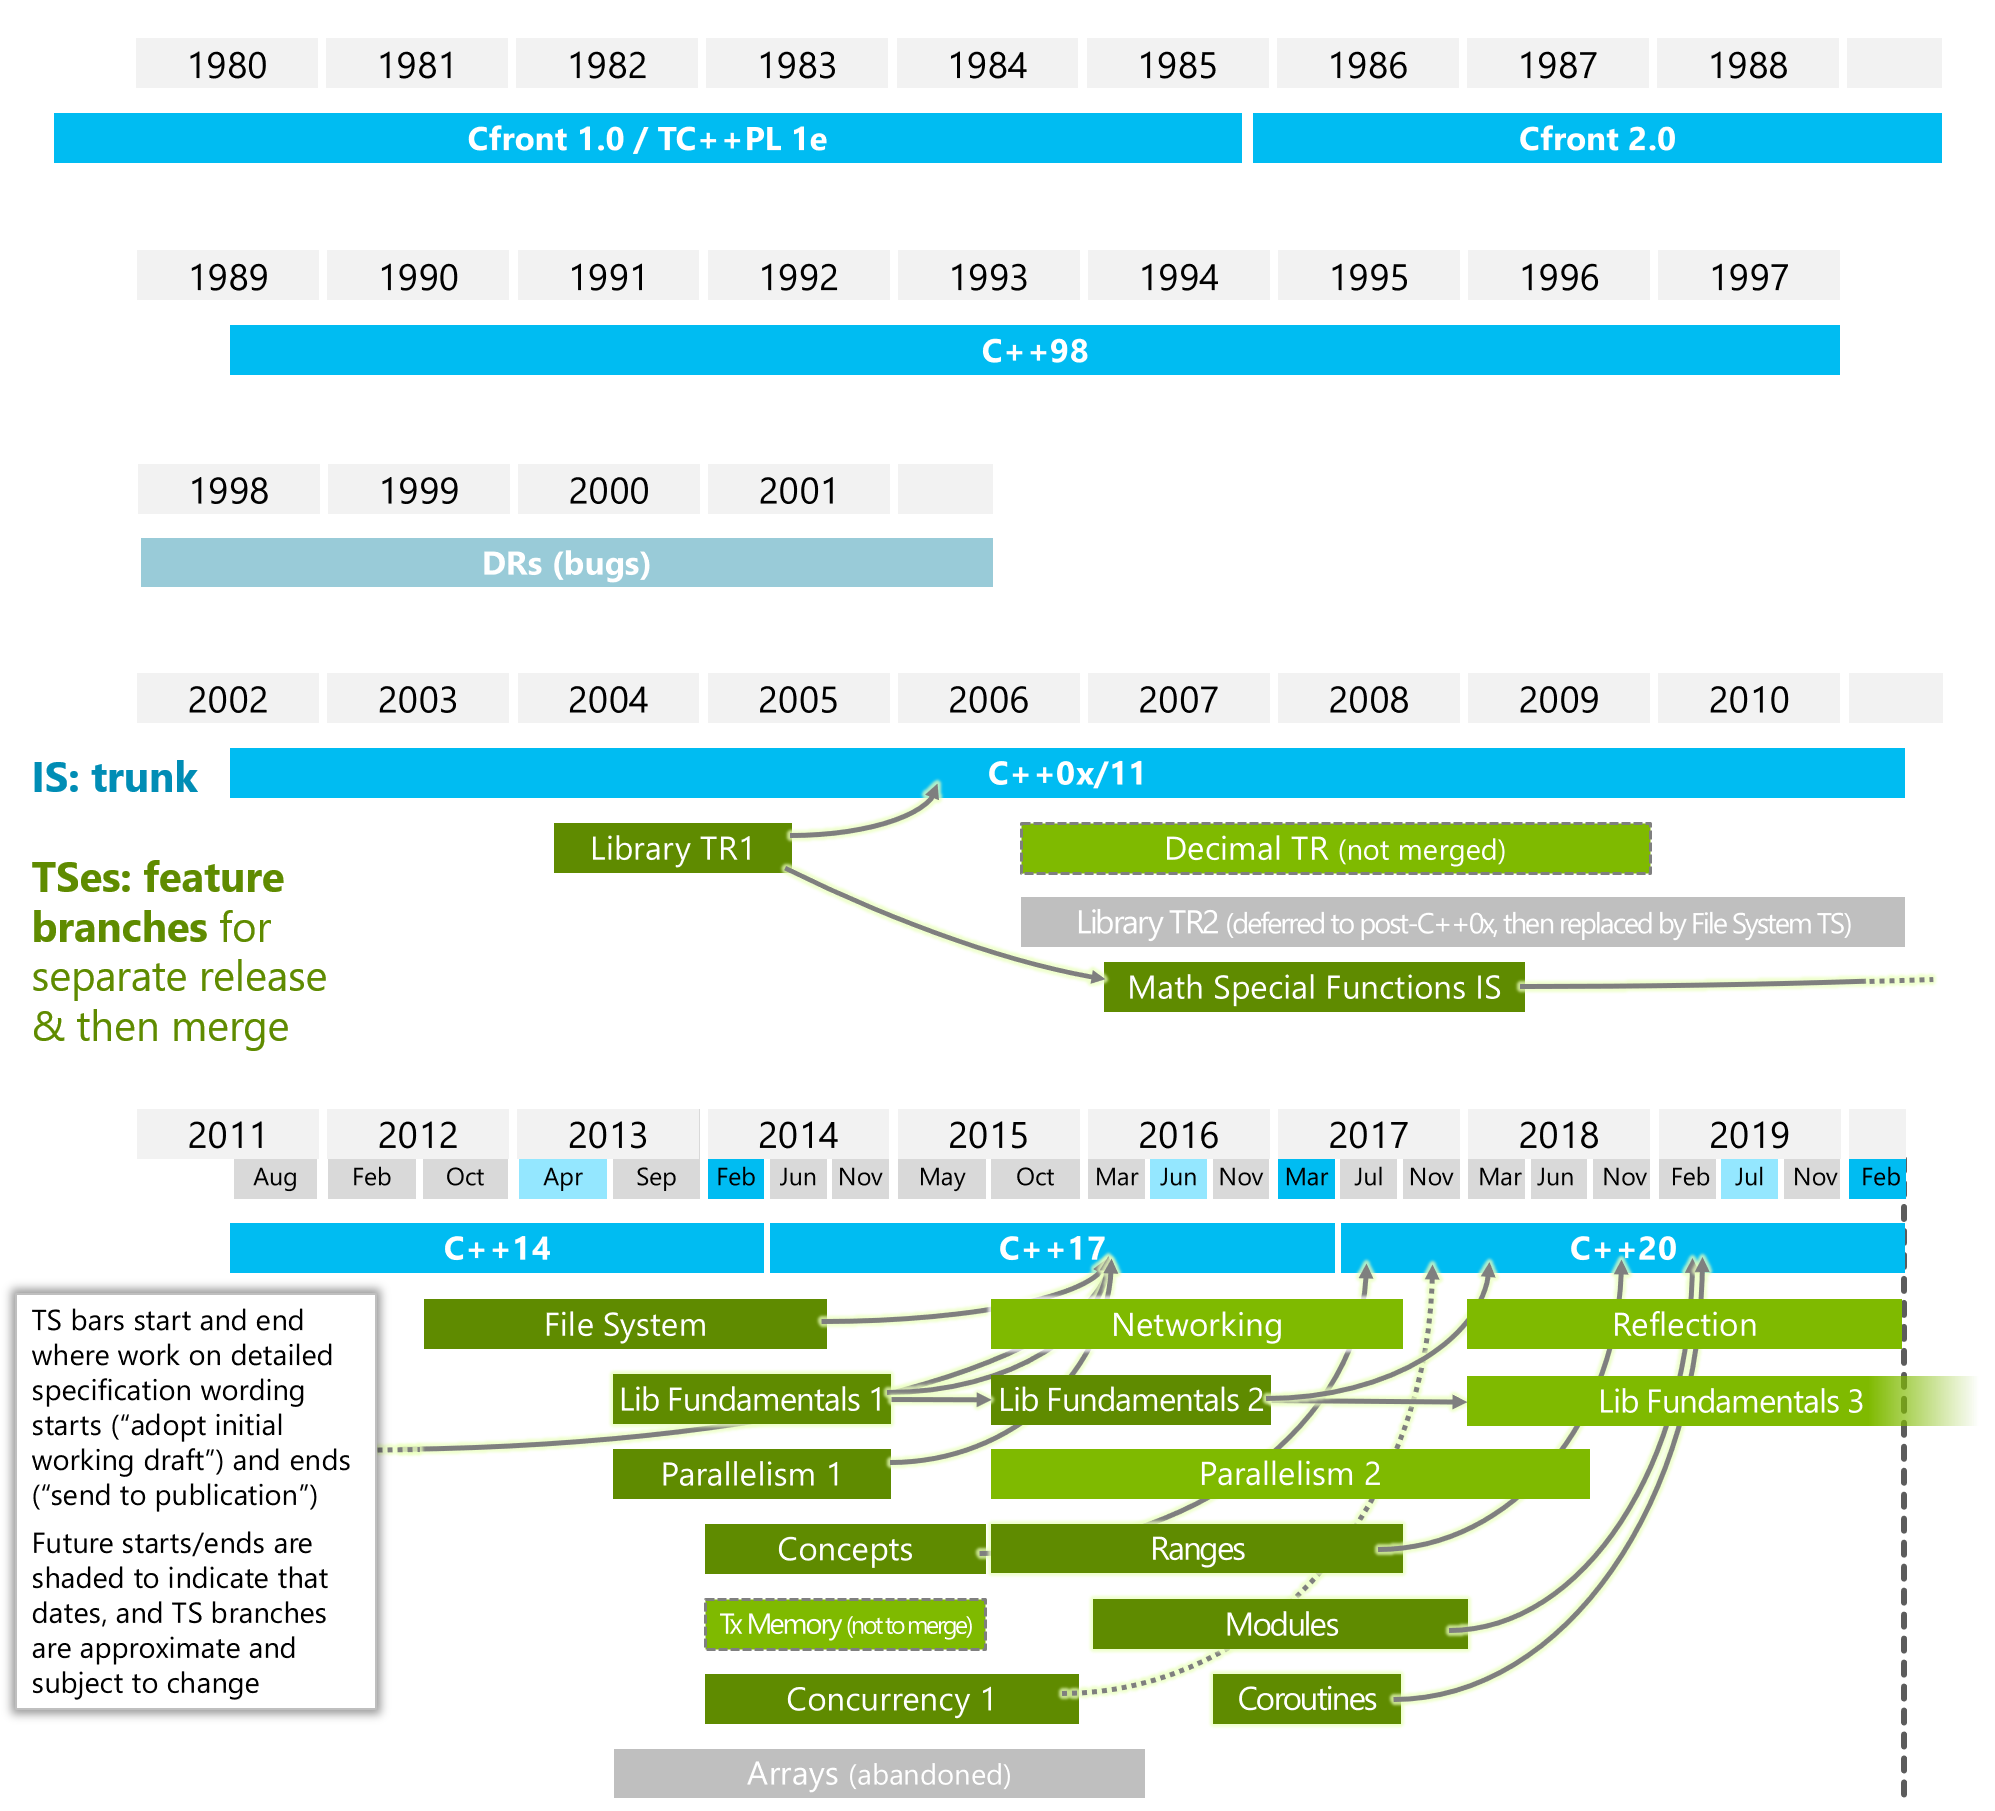
\includegraphics[height=.8\textheight]{images/wg21-timeline-2020.png}
\end{frame}
}

\begin{frame}[t]{Principios de diseño}
\begin{itemize}
  \item \pause  Mantener compatibilidad hacia atrás.
  \item \pause  Mejor extender la biblioteca que el lenguaje.
  \item \pause  Facilitar el diseño de sistemas y bibliotecas (en vez de dominios concretos).
  \item \pause  Mejorar la seguridad de tipos.
  \item \pause  Mejorar el rendimiento y la interacción con el hardware.
  \item \pause  Principio de \emph{zero-overhead}.
  \item \pause  Hacer C++ más fácil de enseñar y aprender.
\end{itemize}
\end{frame}


\section{Un primer programa}

\begin{frame}{Hola}
\begin{columns}

\column{ .5\textwidth}
\begin{block}{hola.cpp}
\lstinputlisting{01-introcpp/hola/hola.cpp}
\end{block}

\column{.5\textwidth}
  \begin{itemize}
    \item Archivo de cabecera: \mode<presentation>{\cppid{iostream}.}
      \mode<article>{
        \begin{itemize}
          \item Se sigue el paradigma de sustitución de texto.
        \end{itemize}
      }
    \item Importación de espacio de nombres: \mode<presentation>{\cppid{std}.}
      \mode<article>{
        \begin{itemize}
          \item Alcance que contiene elementos de una biblioteca para evitar conflictos de nombrado.
          \item Es distinto de los modelos de \emph{paquetes} de otros lenguajes.
        \end{itemize}
      }
    \item Programa principal: \mode<presentation>{\cppid{main}.}
      \mode<article>{
        \begin{itemize}
          \item Es el punto de entrada al programa.
          \item Hay cosas que ocurren antes.
          \item Hay cosas que ocurren después.
        \end{itemize}
      }
    \item Flujo de salida estándar: \mode<presentation>{\cppid{cout}.}
      \mode<article>{
        \begin{itemize}
          \item Es una variable global.
        \end{itemize}
      }
    \item Operador de salida: \mode<presentation>{\cppkey{<{}<}.}
      \mode<article>{
        \begin{itemize}
          \item Operador para enviar datos a la salida estándar.
          \item Definido para la mayoría de los tipos.
        \end{itemize}
      }
    \item Salto de línea: \mode<presentation>{\cppid{endl}.}
      \mode<article>{
        \begin{itemize}
          \item Equivalente a \cppid{"\\endl"}.
        \end{itemize}
      }
    \item Código de salida: \mode<presentation>{\cppid{0}.}
      \mode<article>{
        \begin{itemize}
          \item Devuleto al sistema operativo.
        \end{itemize}
      }
  \end{itemize}

\end{columns}
\end{frame}

\subsection{Compilación y enlace}

\begin{frame}[t]{Fases de la traducción}
\begin{itemize}
  \item Preprocesado:
    \begin{itemize}
      \item Procesa las directivas del compilador de una unidad de traducción.
    \end{itemize}
  \vfill
  \item Compilación:
    \begin{itemize}
      \item Traduce el código fuente a código ensamblador.
    \end{itemize}
  \vfill
  \item Ensamblado:
    \begin{itemize}
      \item Ensambla a código objeto.
      \item Normalmente integrada con compilación.
    \end{itemize}
  \vfill
  \item Enlazado:
    \begin{itemize}
      \item Resuelve referencias externas entre módulos objeto.
    \end{itemize}
\end{itemize}
\end{frame}

\begin{frame}[fragile]{El preprocesador}
\begin{columns}

\column{.5\textwidth}
\begin{tikzpicture}
\tikzset{
    archfuente/.style={rectangle,rounded corners,draw=black, top color=white, bottom color=blue!50,very thick, inner sep=0.5em, minimum size=0, text centered, font=\tiny},
    flecha/.style={->, >=latex', shorten >=1pt, thick},
    etiqueta/.style={text centered, font=\tiny} 
}  
\node[archfuente] (cab1) {arch1};
\node[right=1cm of cab1] (cab2) {...};
\node[archfuente, right=1cm of cab2] (cab3) {archN};
\node[archfuente, below =1cm of cab2] (iostream) {\cppid{iostream}};
\draw[flecha] (iostream) -- (cab1);
\draw[flecha] (iostream) -- (cab2);
\draw[flecha] (iostream) -- (cab3);
\node[etiqueta, below =0.1cm of cab1] {\emph{include}};
\node[etiqueta, below left =0.25cm and -0.3cm of cab2] {\emph{include}};
\node[etiqueta, below =0.1cm of cab3] {\emph{include}};
\node[archfuente, below=1cm of iostream] (holacpp) {\cppid{hola.cpp}};
\draw[flecha] (holacpp) -- (iostream);
\node[etiqueta,below left=0.1cm and -0.6cm of iostream] {\emph{include}};
\end{tikzpicture}

\pause
\column{.5\textwidth}
\begin{tikzpicture}
\tikzset{
    archfuente/.style={rectangle,rounded corners,draw=black, top color=white, bottom color=blue!50,very thick, inner sep=5em, minimum size=0, text centered, font=\tiny},
}  
\node[archfuente] () {hola.ii};
\end{tikzpicture}

\end{columns}
\begin{lstlisting}[style=terminal]
g++ hola.cpp -E -o hola.ii
\end{lstlisting}
\begin{itemize}
  \item 17524 líneas.
\end{itemize}
\end{frame}

\begin{frame}[fragile]{Compilación y ensamblado}
\begin{itemize}
\item \alert{Ensamblado}: Genera código ensamblador de una unidad de traducción.
  \begin{itemize}
    \item Es necesario ensamblar el código para llegar a código objeto
\begin{lstlisting}[style=terminal]
g++ hola.cpp -S -o hola.s
\end{lstlisting}
    \item 83 líneas.
  \end{itemize}
\item \pause \alert{Compilación}:Traduce a código objeto.
  \begin{itemize}
    \item Genera ensamblador.
    \item Ensambla a código ejecutable binario.
    \item Dejar sin resolver referencias externas.
  \end{itemize}
\begin{lstlisting}[style=terminal]
g++ hola.cpp -c -o hola.o
\end{lstlisting}
\end{itemize}
\end{frame}

\begin{frame}{Código ensamblador}
\begin{block}{hola.s}
\ldots
\mode<presentation>{
\lstinputlisting[language={[x86masm]Assembler},basicstyle=\tiny\ttfamily,firstline=10,lastline=28]{01-introcpp/hola/hola.s}
}
\mode<article>{
\lstinputlisting[language={[x86masm]Assembler},basicstyle=\ttfamily,firstline=10,lastline=28]{01-introcpp/hola/hola.s}
}
\ldots
\end{block}
\end{frame}

\begin{frame}[fragile]{Ensamblado}
\begin{itemize}
\item \pause Herramientas:
  \begin{itemize}
    \item Lista de símbolos de un archivo objeto:
\begin{lstlisting}[style=terminal]
nm hola.o
\end{lstlisting}
    \item \pause Código ensamblador de secciones ejecutables.
\begin{lstlisting}[style=terminal]
objdump -d hola.o
\end{lstlisting}
    \item \pause Información sobre las secciones del módulo objeto.
\begin{lstlisting}[style=terminal]
readelf -all hola.o
\end{lstlisting}
    \item \pause Si se quiere descifrar los nombres C++, se usa \verb-c++filt-.
\begin{lstlisting}[style=terminal]
nm hola.o | c++filt
\end{lstlisting}
  \end{itemize}
\end{itemize}
\end{frame}

\begin{frame}{Símbolos}
\begin{block}{nm hola.o}
\lstinputlisting[style=terminal,basicstyle=\tiny\ttfamily]{01-introcpp/hola/hola.nm}
\end{block}
\end{frame}

\begin{frame}{Símbolos con nombres descrifrados}
\begin{block}{nm hola.o | c++filt}
\lstinputlisting[style=terminal,basicstyle=\tiny\ttfamily]{01-introcpp/hola/hola.nm.cpp}
\end{block}
\end{frame}

\begin{frame}{Enlace}
\begin{itemize}
\item Resuelve referencias externas entre módulos objeto.
\item Genera programa ejecutable.
\end{itemize}
\begin{tikzpicture}
\tikzset{
    archfuente/.style={rectangle,rounded corners,draw=black, top color=white, bottom color=blue!50,very thick, inner sep=0.5em, minimum size=0, text centered, font=\tiny},
    flecha/.style={->, >=latex', shorten >=1pt, thick},
    etiqueta/.style={text centered, font=\tiny} 
}  
\node[archfuente] (cab1) {arch1};
\node[right=1cm of cab1] (cab2) {...};
\node[archfuente, right=1cm of cab2] (cab3) {archN};
\node[archfuente, below =1cm of cab2] (iostream) {\cppid{iostream}};
\draw[flecha] (iostream) -- (cab1);
\draw[flecha] (iostream) -- (cab2);
\draw[flecha] (iostream) -- (cab3);
\node[etiqueta, below =0.1cm of cab1] {\emph{include}};
\node[etiqueta, below left =0.25cm and -0.3cm of cab2] {\emph{include}};
\node[etiqueta, below =0.1cm of cab3] {\emph{include}};
\node[archfuente, below=1cm of iostream] (holacpp) {\cppid{hola.cpp}};
\draw[flecha] (holacpp) -- (iostream);
\node[etiqueta,below left=0.1cm and -0.6cm of iostream] {\emph{include}};
\node[archfuente,right=2cm of iostream] (holao) {\cppid{hola.o}};
\node[etiqueta,right=0.1cm of holao] {\emph{enlace}};
\draw[flecha] (holacpp) -- (holao);
\node[etiqueta,above right=0.1cm and 0.6cm of holacpp] {\emph{compilación}};
\node[archfuente,right=2cm of holacpp] (stdlib) {\cppid{libstdc++}};
\node[etiqueta,right=0.1cm of stdlib] {\emph{enlace}};
\node[archfuente,below right=0.5cm and 1cm of holao] (hola) {\cppid{hola}};
\draw[flecha] (holao) -- (hola);
\draw[flecha] (stdlib) -- (hola);
\end{tikzpicture}
\end{frame}

\subsection{Entornos de programación}

\begin{frame}[t]{Línea de comandos versus entornos integrados}
\begin{itemize}
  \item Línea de comandos:
    \begin{itemize}
      \item Editor para la edición de archivos fuentes (\emph{vim/gvim}, \emph{gedit}, \emph{emacs}, \ldots).
      \item Compilador (\textmark{\emph{g++}}, \emph{clang}, \ldots).
      \item Depurador.
      \item \ldots
    \end{itemize}
  \vfill
  \item Entornos integrados:
    \begin{itemize}
      \item Eclipse/CDT.
      \item Code::Blocks.
      \item KDevelop.
      \item Visual Studio.
      \item \textmark{CLion}.
    \end{itemize}
\end{itemize}
\end{frame}


\mode<article>{\chapter{\modulehello}}

\mode<presentation>{\begin{frame}[shrink=20]{Licencia Creative Commons}

\begin{tabularx}{.98\textwidth}{lX}
\ccLogo & Este trabajo se distribuye bajo licencia
Atribución-NoComercial-SinDerivadas 4.0 Internacional (CC BY-NC-ND 4.0).\\

&\\

& \multicolumn{1}{c}{\textbf{Usted es libre de}:}\\

&\\

&
\textbf{Compartir} --
copiar y redistribuir el material en cualquier medio o formato.
\\

&\\

& \multicolumn{1}{c}{\textbf{Bajo los siguientes términos}:}\\

&\\

\ccAttribution &
Atribución -- Usted debe dar crédito de manera adecuada, brindar un enlace a la licencia, e indicar si se han realizado cambios. Puede hacerlo en cualquier forma razonable, pero no de forma tal que sugiera que usted o su uso tienen el apoyo de la licenciante.
\\

\ccNonCommercialEU &
NoComercial -- Usted no puede hacer uso del material con propósitos comerciales. 
\\

\ccNoDerivatives &
SinDerivadas -- Si remezcla, transforma o crea a partir del material, no podrá distribuir el material modificado. 
\\

\end{tabularx}

\end{frame}
}
\section{Un primer programa}

\begin{frame}{Hola}
\begin{columns}

\column{ .5\textwidth}
\begin{block}{hola.cpp}
\lstinputlisting{ejemplos/02-hola/hola/hola.cpp}
\end{block}

\column{.5\textwidth}
  \begin{itemize}
    \item Archivo de cabecera: \mode<presentation>{\cppid{iostream}.}
      \mode<article>{
        \begin{itemize}
          \item Se sigue el paradigma de sustitución de texto.
        \end{itemize}
      }
    \item Programa principal: \mode<presentation>{\cppid{main}.}
      \mode<article>{
        \begin{itemize}
          \item Es el punto de entrada al programa.
          \item Hay cosas que ocurren antes.
          \item Hay cosas que ocurren después.
        \end{itemize}
      }
    \item Importación de espacio de nombres: \mode<presentation>{\cppid{std}.}
      \mode<article>{
        \begin{itemize}
          \item Alcance que contiene elementos de una biblioteca para evitar conflictos de nombrado.
          \item Es distinto de los modelos de \emph{paquetes} de otros lenguajes.
        \end{itemize}
      }
    \item Flujo de salida estándar: \mode<presentation>{\cppid{cout}.}
      \mode<article>{
        \begin{itemize}
          \item Es una variable global.
        \end{itemize}
      }

    \mode<article>{\clearpage}
    \item Operador de salida: \mode<presentation>{\cppkey{<{}<}.}
      \mode<article>{
        \begin{itemize}
          \item Operador para enviar datos a la salida estándar.
          \item Definido para la mayoría de los tipos.
        \end{itemize}
      }
    \item Salto de línea: \mode<presentation>{\cppid{endl}.}
      \mode<article>{
        \begin{itemize}
          \item Equivalente a \cppid{"\textbackslash{}n"}.
        \end{itemize}
      }
    \item Código de salida: \mode<presentation>{\cppid{0}.}
      \mode<article>{
        \begin{itemize}
          \item Devuleto al sistema operativo.
        \end{itemize}
      }
  \end{itemize}

\end{columns}
\end{frame}

\subsection{Compilación y enlace}

\begin{frame}[t]{Fases de la traducción}
\begin{itemize}
  \item \textgood{Preprocesado}:
    \begin{itemize}
      \item Procesa las \textmark{directivas del compilador} de una unidad de traducción.
    \end{itemize}

  \mode<presentation>{\vfill}
  \item \textgood{Compilación}:
    \begin{itemize}
      \item \textmark{Traduce} el código fuente a código ensamblador.
    \end{itemize}

  \mode<presentation>{\vfill}
  \item \textgood{Ensamblado}:
    \begin{itemize}
      \item Ensambla a \textmark{código objeto}.
      \item Normalmente integrada con compilación.
    \end{itemize}

  \mode<presentation>{\vfill}
  \item \textgood{Enlazado}:
    \begin{itemize}
      \item Resuelve \textmark{referencias externas} entre módulos objeto.
    \end{itemize}
\end{itemize}
\end{frame}

\begin{frame}[fragile]{El preprocesador}
\begin{columns}

\column{.5\textwidth}
\begin{tikzpicture}
\tikzset{
    archfuente/.style={rectangle,rounded corners,draw=black, top color=white, bottom color=blue!50,very thick, inner sep=0.5em, minimum size=0, text centered, font=\tiny},
    flecha/.style={->, >=latex', shorten >=1pt, thick},
    etiqueta/.style={text centered, font=\tiny} 
}  
\node[archfuente] (cab1) {arch1};
\node[right=1cm of cab1] (cab2) {...};
\node[archfuente, right=1cm of cab2] (cab3) {archN};
\node[archfuente, below =1cm of cab2] (iostream) {\cppid{iostream}};
\draw[flecha] (iostream) -- (cab1);
\draw[flecha] (iostream) -- (cab2);
\draw[flecha] (iostream) -- (cab3);
\node[etiqueta, below =0.1cm of cab1] {\emph{include}};
\node[etiqueta, below left =0.25cm and -0.3cm of cab2] {\emph{include}};
\node[etiqueta, below =0.1cm of cab3] {\emph{include}};
\node[archfuente, below=1cm of iostream] (holacpp) {\cppid{hola.cpp}};
\draw[flecha] (holacpp) -- (iostream);
\node[etiqueta,below left=0.1cm and -0.6cm of iostream] {\emph{include}};
\end{tikzpicture}

\pause
\column{.5\textwidth}
\begin{tikzpicture}
\tikzset{
    archfuente/.style={rectangle,rounded corners,draw=black, top color=white, bottom color=blue!50,very thick, inner sep=5em, minimum size=0, text centered, font=\tiny},
}  
\node[archfuente] () {hola.ii};
\end{tikzpicture}

\end{columns}
\begin{lstlisting}[style=terminal]
g++ hola.cpp -E -o hola.ii
\end{lstlisting}
\begin{itemize}
  \item 30,015 líneas (g++ 10.2).
\end{itemize}
\end{frame}

\begin{frame}[fragile]{Compilación y ensamblado}
\begin{itemize}
\item \textgood{Ensamblado}: Genera código ensamblador de una unidad de traducción.
  \begin{itemize}
    \item Es necesario ensamblar el código para llegar a código objeto
\begin{lstlisting}[style=terminal]
g++ hola.cpp -S -o hola.s
\end{lstlisting}
    \item 116 líneas de ensamblador (g++ 10.2).
  \end{itemize}
\item \pause \textgood{Compilación}:Traduce a código objeto.
  \begin{itemize}
    \item Genera ensamblador.
    \item Ensambla a código ejecutable binario.
    \item Dejar sin resolver referencias externas.
  \end{itemize}
\begin{lstlisting}[style=terminal]
g++ hola.cpp -c -o hola.o
\end{lstlisting}
\end{itemize}
\end{frame}

\begin{frame}{Código ensamblador}
\begin{block}{hola.s}
\ldots
\mode<presentation>{
\lstinputlisting[language={[x86masm]Assembler},basicstyle=\tiny\ttfamily,firstline=10,lastline=28]{ejemplos/02-hola/hola/hola.s}
}
\mode<article>{
\lstinputlisting[language={[x86masm]Assembler},basicstyle=\ttfamily,firstline=10,lastline=28]{ejemplos/02-hola/hola/hola.s}
}
\ldots
\end{block}
\end{frame}

\begin{frame}[fragile]{Ensamblado}
\begin{itemize}
\item \pause Herramientas:
  \begin{itemize}
    \item Lista de símbolos de un archivo objeto:
\begin{lstlisting}[style=terminal]
nm hola.o
\end{lstlisting}
    \item \pause Código ensamblador de secciones ejecutables.
\begin{lstlisting}[style=terminal]
objdump -d hola.o
\end{lstlisting}
    \item \pause Información sobre las secciones del módulo objeto.
\begin{lstlisting}[style=terminal]
readelf -all hola.o
\end{lstlisting}
    \item \pause Si se quiere descifrar los nombres C++, se usa \verb-c++filt-.
\begin{lstlisting}[style=terminal]
nm hola.o | c++filt
\end{lstlisting}
  \end{itemize}
\end{itemize}
\end{frame}

\begin{frame}{Símbolos}
\begin{block}{nm hola.o}
\lstinputlisting[style=terminal,basicstyle=\tiny\ttfamily]{ejemplos/02-hola/hola/hola.nm}
\end{block}
\end{frame}

\begin{frame}{Símbolos con nombres descrifrados}
\begin{block}{nm hola.o | c++filt}
\lstinputlisting[style=terminal,basicstyle=\tiny\ttfamily]{ejemplos/02-hola/hola/hola.nm.cpp}
\end{block}
\end{frame}

\begin{frame}{Enlace}
\begin{itemize}
\item Resuelve referencias externas entre módulos objeto.
\item Genera programa ejecutable.
\end{itemize}
\begin{tikzpicture}
\tikzset{
    archfuente/.style={rectangle,rounded corners,draw=black, top color=white, bottom color=blue!50,very thick, inner sep=0.5em, minimum size=0, text centered, font=\tiny},
    flecha/.style={->, >=latex', shorten >=1pt, thick},
    etiqueta/.style={text centered, font=\tiny} 
}  
\node[archfuente] (cab1) {arch1};
\node[right=1cm of cab1] (cab2) {...};
\node[archfuente, right=1cm of cab2] (cab3) {archN};
\node[archfuente, below =1cm of cab2] (iostream) {\cppid{iostream}};
\draw[flecha] (iostream) -- (cab1);
\draw[flecha] (iostream) -- (cab2);
\draw[flecha] (iostream) -- (cab3);
\node[etiqueta, below =0.1cm of cab1] {\emph{include}};
\node[etiqueta, below left =0.25cm and -0.3cm of cab2] {\emph{include}};
\node[etiqueta, below =0.1cm of cab3] {\emph{include}};
\node[archfuente, below=1cm of iostream] (holacpp) {\cppid{hola.cpp}};
\draw[flecha] (holacpp) -- (iostream);
\node[etiqueta,below left=0.1cm and -0.6cm of iostream] {\emph{include}};
\node[archfuente,right=2cm of iostream] (holao) {\cppid{hola.o}};
\node[etiqueta,right=0.1cm of holao] {\emph{enlace}};
\draw[flecha] (holacpp) -- (holao);
\node[etiqueta,above right=0.1cm and 0.6cm of holacpp] {\emph{compilación}};
\node[archfuente,right=2cm of holacpp] (stdlib) {\cppid{libstdc++}};
\node[etiqueta,right=0.1cm of stdlib] {\emph{enlace}};
\node[archfuente,below right=0.5cm and 1cm of holao] (hola) {\cppid{hola}};
\draw[flecha] (holao) -- (hola);
\draw[flecha] (stdlib) -- (hola);
\end{tikzpicture}
\end{frame}

\subsection{Entornos de programación}

\begin{frame}[t]{Compiladores}
  \begin{itemize}
    \item \textgood{Compilador}: Conjunto de herramientas para la traducción
          de código fuente.
      \begin{itemize}
        \item Integran compilación, enlace y herramientas auxiliares.
        \item Típicamente línea de comandos
      \end{itemize}

  \mode<presentation>{\vfill}
  \item Algunos \textgood{compiladores}:
    \begin{itemize}
      \item \textmark{Open source}: \textemph{g++}, clang++.
      \item \textmark{Fabricantes hardware}: AMD, ARM, Cray, HP, Intel, NVidia, Oracle, IBM.
      \item \textmark{Solo Windows}: MSVC (Microsoft).
      \item \textmark{Otros}: IAR, C++ Builder, \ldots
    \end{itemize}
  \end{itemize}
\end{frame}

\begin{frame}[t]{Entornos de desarrollo}
\begin{itemize}
  \item \textgood{Entornos integrados}: Integran edición, compilación, depuración
        y muchas más herramientas.

  \mode<presentation>{\vfill}
  \item Algunos \textgood{IDE}.
    \begin{itemize}
      \item \textmark{Open Source}: Code::Blocks, Dev-C++, Eclipse/CDT, KDevelop.
      \item \textmark{Microsoft}: Visual Studio, Visual Studio Code (varias plataformas).
      \item \textmark{MacOS}: XCode.
      \item \textmark{Otros}: QtCreator, \textemph{CLion}, \ldots
    \end{itemize}
\end{itemize}
\end{frame}


\mode<article>{
  \section{Lecturas recomendadas}

\begin{enumerate}

\item Lee el capítulo 2 (\emph{Hello, World!}) de \pppbook{}
      para seguir paso a paso la creación de un programa.

\end{enumerate}

  \section{Ejercicios}

\begin{enumerate}

\item Si no tienes acceso a un sistema Linux, instala una versión reciente de Linux.
Se recomienda utilizar, por ejemplo, Ubuntu Linux. Sigue los pasos en el tutorial
suministrado por Ubuntu en la siguiente URL:

  \begin{itemize}
    \item \url{https://ubuntu.com/tutorials/install-ubuntu-desktop#1-overview}.
  \end{itemize}

\item Asegúrate de instalar la versión 10 de \cppid{g++}:

\begin{lstlisting}[style=terminal]
sudo add-apt-repository ppa:ubuntu-toolchain-r/test
sudo apt-get update
sudo apt install gcc-10
sudo apt install g++-10
\end{lstlisting}

\item Edita el programa en un archivo con el nombre \cppid{hola.cpp}. Desde la 
línea de comandos ejecuta la siguiente línea para compilar el programa:

\begin{lstlisting}[style=terminal]
g++ hola.cpp -o hola
\end{lstlisting}

Ejecuta el programa resultante.

\item Obten una licencia para estudiantes del entorno de desarrollo \textmark{CLion}
en la siguiente URL:
\begin{itemize}
  \item \url{https://www.jetbrains.com/es-es/community/education/#students}
\end{itemize}

\item Ejecuta el entorno de desarrollo \textmark{CLion} y sigue los siguiente pasos:

\begin{enumerate}
\item Crea un proyecto con las siguientes características:
\begin{itemize}
  \item \textmark{Project type}: C++ Executable.
  \item \textmark{Language standard}: C++20.
\end{itemize}

\item Comprueba que se generan los siguientes archivos:
\begin{itemize}
  \item \cppid{main.cpp}.
  \item \cppid{CMakeLists.txt}
\end{itemize}

\item Construye el programa mediante la opción \textmark{Build | Build Project}. 
Comprueba que el programa se construye correctamente.

\item Ejecuta el programa (\textmark{Run | Run 'hola'}).
Comprueba que el programa se ejecuta correctamente. La salida debería ser:

\begin{lstlisting}[style=terminal]
Hello, World!

Process finished with exit code 0
\end{lstlisting}

\end{enumerate}

\end{enumerate}

}

\mode<article>{\chapter{\modulevalues}}

\mode<presentation>{\begin{frame}[shrink=20]{Licencia Creative Commons}

\begin{tabularx}{.98\textwidth}{lX}
\ccLogo & Este trabajo se distribuye bajo licencia
Atribución-NoComercial-SinDerivadas 4.0 Internacional (CC BY-NC-ND 4.0).\\

&\\

& \multicolumn{1}{c}{\textbf{Usted es libre de}:}\\

&\\

&
\textbf{Compartir} --
copiar y redistribuir el material en cualquier medio o formato.
\\

&\\

& \multicolumn{1}{c}{\textbf{Bajo los siguientes términos}:}\\

&\\

\ccAttribution &
Atribución -- Usted debe dar crédito de manera adecuada, brindar un enlace a la licencia, e indicar si se han realizado cambios. Puede hacerlo en cualquier forma razonable, pero no de forma tal que sugiera que usted o su uso tienen el apoyo de la licenciante.
\\

\ccNonCommercialEU &
NoComercial -- Usted no puede hacer uso del material con propósitos comerciales. 
\\

\ccNoDerivatives &
SinDerivadas -- Si remezcla, transforma o crea a partir del material, no podrá distribuir el material modificado. 
\\

\end{tabularx}

\end{frame}
}
\section{Variables, valores y tipos}

\begin{frame}[t,fragile]{Variables, valores y objetos}
\begin{lstlisting}
int x = 65;
\end{lstlisting}
\begin{itemize}
  \item \textmark{Variable}: Nombre de un objeto en un programa.
    \begin{itemize}
      \item \cppid{x} es una variable.
    \end{itemize}

  \mode<presentation>{\vfill}
  \item \textmark{Valor}: Secuencia de bits que se interpreta de acuerdo con las reglas de un tipo.
    \begin{itemize}
      \item El valor \verb+00000000 00000000 00000000 01000001+ represetan el número \cppid{65} para el tipo \cppkey{int}.
      \item El valor \verb+01000001+ represetna el carácter \cppid{'A'} para el tipo \cppkey{char}.
    \end{itemize}

  \mode<presentation>{\vfill}
  \item \textmark{Objeto}: Secuencia de uno o más \emph{bytes} que contiene un valor de un tipo.
    \begin{itemize}
      \item Un objeto es lugar en la memoria en que se almacena un valor.
      \item Una variable permite referenciar un objeto.
        \mode<article>{
          \item \textmark{IMPORTANTE}: El concepto de objeto no tiene que ver necesariamente con la \emph{orientación a objetos}.
        }
    \end{itemize}
\end{itemize}
\end{frame}

\begin{frame}[t]{Tipo}
\begin{itemize}
  \item \textmark{Tipo}: Definición del conjunto de valores y operaciones admisibles para un objeto.
    \begin{itemize}

      \mode<presentation>{\vfill}
      \item \textmark{Tipos fundamentales}: Definidos por el lenguaje.
        \begin{itemize}
          \item \textmark{\emph{Booleanos}}: \cppkey{bool}.
          \item \textmark{Carácter}: \cppkey{char}, \cppkey{signed char}, \cppkey{unsigned char}, \cppkey{wchar\_t}, \cppkey{char16\_t}, \cppkey{char32\_t}.
          \item \textmark{Enteros}: \cppkey{short}, \cppkey{int}, \cppkey{long}, \cppkey{long long}.
            \mode<article>{
              \begin{itemize}
                \item Pueden llevar prefijo \cppkey{signed} o \cppkey{unsigned}.
                \item Si no se indica nada, se toma \cppkey{signed}.
              \end{itemize}
            }
          \item \textmark{Coma flotante}: \cppkey{float}, \cppkey{double}, \cppkey{long double}.
        \end{itemize}

      \mode<presentation>{\vfill}
      \item \textmark{Tipos predefinidos}: Definidos por al biblioteca estándar.
        \begin{itemize}
          \item Algunos ejemplos \cppid{string}, \cppid{vector}, \ldots
        \end{itemize}

      \mode<presentation>{\vfill}
      \item \textmark{Tipos definidos por el usuario}: Definidos por otra biblioteca o por el programa.
    \end{itemize}
\end{itemize}
\end{frame}

\begin{frame}[t,fragile]{\texttt{bool}}
\begin{itemize}
  \item Literales: \cppkey{false} y \cppkey{true}.
  \item Operaciones:
    \begin{itemize}
      \item Asignación.
\begin{lstlisting}
x = true;
\end{lstlisting}
      \item Comparación de igualdad.
\begin{lstlisting}
bool b1=true, b2=false;
x = {b1 == b2};
x = {b1 != b2};
\end{lstlisting}
      \item Comparación relacional
\begin{lstlisting}
bool b1=true, b2=false;
x = {b1 < b2};
x = {b1 <= b2};
x = {b1 > b2};
x = {b1 >= b2};
\end{lstlisting}
    \end{itemize}
\end{itemize}
\end{frame}

\begin{frame}[t,fragile]{Tipos carácter}
\begin{itemize}
  \item Literales entre comillas simples son de tipo \cppkey{char}.
    \begin{itemize}
      \item \cppid{'a'}, \cppid{'x'}, \ldots
      \mode<article>{
        \item También hay formatos para literales \cppkey{char16\_t}, \cppkey{char32\_t} y \cppkey{wchar\_t}.
      }
    \end{itemize}
  \item Secuencias de escape para caracteres especiales:
    \begin{itemize}
      \item Caracteres especiales: \cppkey{\textbackslash{}n}, \cppkey{\textbackslash{}r}, 
        \cppkey{\textbackslash{}t}, \cppkey{\textbackslash{}v},
        \cppkey{\textbackslash{}b}, \cppkey{\textbackslash{}f}, 
        \cppkey{\textbackslash{}a}.
      \item Secuencias de escape:
        \cppkey{\textbackslash{}\textbackslash}, 
        \cppkey{\textbackslash{}?}, 
        \cppkey{\textbackslash{}'}, 
        \cppkey{\textbackslash{}''}, 
    \end{itemize}
  \item Operaciones:
    \begin{itemize}
      \item Asignación.
\begin{lstlisting}
x = 'a';
\end{lstlisting}
      \item Comparaciones.
\begin{lstlisting}
bool b;
char c1 = 'a', c2 = 'b';
b = { c1 != c2};
b = { c1 >= c2};
\end{lstlisting}
    \end{itemize}
\end{itemize}
\end{frame}

\begin{frame}[t]{Tipos enteros}
\begin{itemize}
  \item \textgood{Literales}:
    \begin{itemize}

      \mode<presentation>{\vfill}
      \item \textmark{Base} en los literales:
        \begin{itemize}
          \item \cppid{1000} $\rightarrow$ Base 10.
          \item \cppid{01000} $\rightarrow$ Base 8.
          \item \cppid{0x1000} $\rightarrow$ Base 16.
        \end{itemize}

      \mode<presentation>{\vfill}
      \item \textmark{Tipo} en los literales:
        \begin{itemize}
          \item \cppid{1234} $\rightarrow$ \cppkey{int}.
          \item \cppid{1234u} $\rightarrow$ \cppkey{unsigned int}.
          \item \cppid{1234l} $\rightarrow$ \cppkey{long int}.
          \item \cppid{1234ul} $\rightarrow$ \cppkey{unsigned long int}.
          \item \cppid{1234ll} $\rightarrow$ \cppkey{long long int}.
          \item \cppid{1234ull} $\rightarrow$ \cppkey{unsigned long long int}.
        \end{itemize}
    \end{itemize}
\end{itemize}
\end{frame}

\begin{frame}[fragile,t]{Operaciones sobre tipos enteros}
\begin{itemize}
      \item \textmark{Asignación}: \cppkey{=}.
\begin{lstlisting}
x = 42;
\end{lstlisting}

      \mode<presentation>{\vfill}
      \item \textmark{Comparaciones}:
        \cppkey{==},
        \cppkey{!=},
        \cppkey{<},
        \cppkey{<=},
        \cppkey{>},
        \cppkey{>=}.

\begin{lstlisting}
int y=2, z=3;
bool b = {x > y};
\end{lstlisting}

      \mode<presentation>{\vfill}
      \item \textmark{Operaciones aritméticas}: 
        \cppkey{+}, \cppkey{-}, \cppkey{*}, \cppkey{/}, \cppkey{\%}.
\begin{lstlisting}
int y=2, z=3;
int x = y + z;
\end{lstlisting}
\end{itemize}
\end{frame}

\begin{frame}[fragile,t]{Operaciones sobre tipos enteros}
\begin{itemize}
  \item \textmark{Operaciones aritméticas con asignación}.
    \cppkey{+=}, \cppkey{-=}, \cppkey{*=}, \cppkey{/=}, \cppkey{\%=}.
\begin{lstlisting}
int y=2, z=3;
y *= z;
\end{lstlisting}

  \mode<presentation>{\vfill}
  \item \textmark{Incremento/decremento}: \cppkey{++}, \cppkey{-{}-}.
\begin{lstlisting}
int n = 10;
int x;
x = ++n;
x = n++;
x = --n;
x = n--;
\end{lstlisting}
\end{itemize}
\end{frame}


\begin{frame}[t,fragile]{Coma flotante}
\begin{itemize}
  \item \textgood{Literales}:
    \begin{itemize}
      \item \cppid{1.5} $\rightarrow$ \cppkey{double}.
      \item \cppid{1.5f} $\rightarrow$ \cppkey{float}.
      \item \cppid{1.5l} $\rightarrow$ \cppkey{long double}.
    \end{itemize}
  \item \textgood{Operaciones}:
\begin{columns}

\column{.5\textwidth}

\begin{itemize}
      \item \textmark{Asignación}.
\begin{lstlisting}
x = 1.5;
\end{lstlisting}
      \item \textmark{Comparaciones}:
        \cppkey{==},
        \cppkey{!=},
        \cppkey{<},
        \cppkey{<=},
        \cppkey{>},
        \cppkey{>=}.
      \item \textmark{Operaciones aritméticas}: 
        \cppkey{+}, \cppkey{-}, \cppkey{*}, \cppkey{/}.
\begin{lstlisting}
double y=2.5, z=1.5;
double x = y + z;
\end{lstlisting}
\end{itemize}

\column{.5\textwidth}

\begin{itemize}
      \item \textmark{Operaciones aritméticas con asignación}:
        \cppkey{+=}, \cppkey{-=}, \cppkey{*=}, \cppkey{/=}.
\begin{lstlisting}
double y=2.5, z=1.5;
y *= z;
\end{lstlisting}
      \item \textmark{Incremento/decremento}: \cppkey{++}, \cppkey{-{}-}.
\begin{lstlisting}
double x=1.5;
x++;
\end{lstlisting}
\end{itemize}

\end{columns}
\end{itemize}
\end{frame}

\begin{frame}[t,fragile]{Cadenas (\texttt{std::string})}
\begin{itemize}
  \item \textgood{Literales}:
    \begin{itemize}
      \item Entre comillas dobles: \cppid{"Hola"}
    \end{itemize}

  \mode<presentation>{\vfill}
  \item \textgood{Operaciones}:
    \begin{itemize}
      \item \textmark{Asignación}:
\begin{lstlisting}
string x;
x = "Hola";
\end{lstlisting}
      \item \textmark{Concatenación}:
\begin{lstlisting}
string n="Daniel", a="Garcia";
string nc = n + c;
string nc2 = n;
nc2 += c;
\end{lstlisting}
      \item \textmark{Comparaciones}:
        \cppkey{==},
        \cppkey{!=},
        \cppkey{<},
        \cppkey{<=},
        \cppkey{>},
        \cppkey{>=}.
    \end{itemize}
\end{itemize}
\end{frame}


\section{Entrada salida básica}

\begin{frame}[fragile]{Entrada/salida estándar}
\begin{itemize}
  \item Archivo de cabecera: \mode<presentation>{\cppid{<iostream>}}
    \mode<article>{
      \begin{itemize}
        \item Contiene todas las declaraciones de la entrada/salida estándar.
      \end{itemize}
    }
  \item Todas las declaraciones en espacio de nombres \cppid{std}.
  \item Objetos globales:
    \begin{itemize}
      \item \cppid{cin}: Entrada estándar.
      \item \cppid{cout}: Salida estándar.
      \item \cppid{cerr}: Salida de errores.
        \mode<presentation>{
          \begin{itemize}
            \item Va a la salida de errores sin usar un búfer intermedio.
          \end{itemize}
        }
      \item \cppid{clog}: Salida de log.
        \mode<presentation>{
          \begin{itemize}
            \item Va a la salida de errores usando un búfer intermedio.
          \end{itemize}
        }
    \end{itemize}
  \item Operadores:
    \begin{itemize}
      \item Operadores:
        \begin{itemize}
          \item Operador \cppid{<{}<} vuelca un dato en un flujo de salida.
\begin{lstlisting}
std::cout << x;
\end{lstlisting}
          \item Operador \cppid{>>} vuelca un dato en un flujo de entrada.
\begin{lstlisting}
std::cin >> x;
\end{lstlisting}
        \end{itemize}
    \end{itemize}
\end{itemize}
\end{frame}

\begin{frame}[fragile]{Ejemplo}
\begin{block}{main1.cpp}
\lstinputlisting{03-valores/hola-nombre/main1.cpp}
\end{block}
\begin{itemize}
  \item Declaraciones en espacio de nombres \cppid{std}.
    \mode<article>{
      \begin{itemize}
        \item Todos los símbolos de la biblioteca estándar están en este espacio de nombres.
      \end{itemize}
    }
  \item Cadena: Tipo de biblioteca \cppid{string}.
    \mode<article>{
      \begin{itemize}
        \item Es una \emph{clase} definida en la biblioteca estándar.
        \item C++ también tiene el tipo \cppkey{char}\cppid{*}, pero \cppid{string}
          ofrece una interfaz más simple que se prefiere.
      \end{itemize}
    }
  \item \cppid{endl}: Valor para fin de línea.
    \mode<article>{
      \begin{itemize}
        \item \cppid{endl} está definido en la biblioteca estándar como un valor
          que se traduce en un salto de línea.
        \item Además fuerza a vaciar el contenido del búfer asociado (\emph{flushing}).
          \begin{itemize}
            \item También se puede usar \cppid{"\textbackslash{}n"}, pero entonces no se vacía el búfer asociado.
          \end{itemize}
      \end{itemize}
    }
\end{itemize}
\end{frame}

\begin{frame}[fragile]{Ejemplo}
\begin{block}{main2.cpp}
\lstinputlisting{03-valores/hola-nombre/main2.cpp}
\end{block}
\begin{itemize}
  \item \cppkey{using namespace} evita repetición de cualificación de nombres.
\end{itemize}
\end{frame}

\section{Conversiones de tipo}

\begin{frame}{Conversiones de tipo}
\begin{itemize}
  \item C++ es más estricto con la seguridad de tipos que C.
  \item \textgood{Conversiones}:
    \begin{itemize}
      \item \textmark{Conversiones seguras}: Se pueden realizar siempre.
        \begin{itemize}
          \item \cppkey{int} $\rightarrow$ \cppkey{long}.
        \end{itemize}
      \item \textmark{Conversiones no seguras}: Problemas en algunos casos.
        \begin{itemize}
          \item \cppkey{long} $\rightarrow$ \cppkey{int}.
        \end{itemize}
    \end{itemize}
  \item \textgood{Conversiones implícitas}:
    \begin{itemize}
      \item Promociones integrales. Ej.: \cppkey{char} $\rightarrow$ \cppkey{int}.
      \item Promoociones de coma flotante. Ej.: \cppkey{float} $\rightarrow$ \cppkey{double}.
      \item Conversiones enteras. Ej. \cppkey{int} $\rightarrow$ \cppkey{long}.
      \item Conversiones de coma flotante. Ej. \cppkey{double} $\rightarrow$ \cppkey{float}.
      \item Conversiones de flotante a entero. Ej. \cppkey{double} $\rightarrow$ \cppkey{int}.
      \item Conversiones de booleanos. Ej. \cppkey{bool} $\rightarrow$ \cppkey{int}.
    \end{itemize}
\end{itemize}
\end{frame}

\begin{frame}[t,fragile]{Conversiones no seguras}
\vspace{-0.5em}
\begin{itemize}
  \item Son conversiones en las que se puede llegar a 
        \textbad{obtener un valor incorrecto}.
\begin{lstlisting}
void f1() {
  int x = 1000000;
  short y = x;
  cout << "f1(): " << x << " , " << y << endl;
}
\end{lstlisting}

  \item \textmark{Posible salida}:
\begin{lstlisting}[language=bash,basicstyle=\footnotesize\ttfamily]
f1(): 1000000 , 16960
\end{lstlisting}

  \item Conversiones \textgood{estrechadoras}.
    \begin{itemize}
      \item Tipo de coma flotante $\rightarrow$ Tipo entero.
      \item \cppkey{long double} $\rightarrow$ \cppkey{double} o \cppkey{float}.
      \item \cppkey{double} $\rightarrow$ \cppkey{float}.
      \item Tipo entero $\rightarrow$ Tipo de coma flotante.
      \item Tipo entero $\rightarrow$ Tipo entero que no puede representar todos los valores del tipo original.
    \end{itemize}
\end{itemize}
\end{frame}

\begin{frame}[t,fragile]{Conversiones estrechadoras e iniciación}
\begin{itemize}
  \item ¿Por qué no se prohiben las conversiones estrechadoras?
    \begin{itemize}
      \item Herencia de C.
      \item Hay muchos usos válidos (p. ej. si se ha validado el valor).
    \end{itemize}

  \mode<presentation>{\vfill}
  \item ¿Por qué no se diagnostican los casos problemáticos?
    \begin{itemize}
      \item No se puede de forma general (p. ej. valor leído de un archivo).
    \end{itemize}

  \mode<presentation>{\vfill}
  \item Sintaxis de \textgood{iniciación uniforme}.
\begin{lstlisting}
  int x1 { 1000000 };
  short x2 { 1000 };
  short x3 { 1000000 }; // Error: narrowing
  short x4 { x1 }; // Error: narrowing
\end{lstlisting}
\end{itemize}
\end{frame}


\section{Expresiones, sentencias y operadores}

\begin{frame}[fragile]{Expresiones}
\begin{itemize}
  \item Una expresión combina otras (sub)-expresiones mediante operadores.
    \begin{itemize}
      \item Asignación: \cppid{x=y}.
      \item Llamada a función: \cppid{f(a)}.
      \item Incremento/Decremento: \cppid{++x}, \cppid{x++}, \cppid{-{}-x}, \cppid{x-{}-}.
      \item Aritméticos: 
        \cppid{-x},
        \cppid{x+y},
        \cppid{x-y},
        \cppid{x*y},
        \cppid{x/y},
        \cppid{x\%y},
      \item Aritmético-asignación:
        \cppid{x+=y},
        \cppid{x-=y},
        \cppid{x*=y},
        \cppid{x/=y},
        \cppid{x\%=y},
      \item Comparación:
        \cppid{x<y},
        \cppid{x<=y},
        \cppid{x>y},
        \cppid{x>=y},
        \cppid{x==y},
        \cppid{x!=y},
      \item Lógicos:
        \cppid{!x},
        \cppid{x\&\&y},
        \cppid{x||y}.
      \item Entrada/salida:
        \cppid{os<{}<x}, \cppid{is>{}>x}.
    \end{itemize}
  \item Cualquier expresión puede ser una sentencia
\begin{lstlisting}
x = y + z * ( x + y * f(z,t));
x1 = x2 = g(z,t);
++x;
\end{lstlisting}
\end{itemize}
\end{frame}

\begin{frame}[t,fragile]{Declaraciones de variable}
\begin{itemize}
  \item Una declaración de variable introduce una variable en un bloque.
\begin{lstlisting}
string mision = "Apolo XI";
\end{lstlisting}
  \item No es necesario (ni recomendable) poner las declaraciones al principio del bloque.
\begin{lstlisting}
void f() {
  double distancia;
  cin >> distancia;
  double tiempo;
  cin >> tiempo;
  double velocidad = distancia / tiempo;
  cout << "Velocidad: " << velocidad << endl;
}  
\end{lstlisting}
  \item ¿Qué pasa con variables sin valor inicial?
    \begin{itemize}
      \item Se quedan sin iniciar (valor no definido).
      \item Es una \textbad{fuente común de errores}.
    \end{itemize}
\end{itemize}
\end{frame}

\begin{frame}[t,fragile]{Inferencia de tipo}
\begin{itemize}
  \item Una declaración de variable con iniciador puede \textmark{deducir automáticamente}
        el tipo de datos de la declaración.
\begin{lstlisting}
auto x = 10; // int x = 10;
auto y = 2.5; // double y = 2.5;
auto z = 1.0f; // float z = 1.0f;
\end{lstlisting}

  \mode<presentation>{\vfill}
  \item La deducción de tipos \textbad{no funciona con cadenas}.
    \begin{itemize}
      \item El literal \cppstr{"Hola"} no es de tipo \cppid{string}.
    \end{itemize}
\begin{lstlisting}
auto c1 = "Hola"; // c1 no es de tipo string
auto c2 = string{"Hola"}; // c2 si es de tipo string
using namespace std::literals;
auto c3 = "Hola"s; // c3 es de tipo string
\end{lstlisting}

  \mode<presentation>{\vfill}
  \item También deduce automáticamente el tipo de expresiones.
\begin{lstlisting}
auto t1 = x + y;
auto t2 = f();
\end{lstlisting}
\end{itemize}
\end{frame}

\begin{frame}[t,fragile]{Constantes}
\begin{itemize}
\item Dos \textgood{alternativas}:
  \begin{itemize}

    \item Variable \textmark{inmutables}:
\begin{lstlisting}
const int max_nodos = 1024;
\end{lstlisting}
      \begin{itemize}
        \item Es una variable que no puede modificarse.
        \item Su valor no se conoce hasta que no comienza a ejecutarse el programa.
      \end{itemize}

    \mode<presentation>{\vfill}
    \item \textmark{Expresiones constantes}:
\begin{lstlisting}
constexpr int max_nodos = 1024;
\end{lstlisting}
      \begin{itemize}
        \item Es un sinónimo para una expresión constante.
        \item Su valor se conoce en tiempo de compilación.
        \item Más apropiado para la mayoría de constantes.
      \end{itemize}
  \end{itemize}

  \mode<presentation>{\vfill}
  \item Rara vez es necesario usar \cppkey{\#define}.
    \begin{itemize}
      \item Sustitución de texto heredada de C.
    \end{itemize}
\end{itemize}
\end{frame}



\mode<article>{
  \section{Lecturas recomendadas}

\begin{itemize}

\item Lee el capítulo 3 (\emph{Objects, Types, and values} de~\cite{stroustrup:2014}
      para compelementar los conceptos de objeto, tipo y valor.

\item Lee las secciones 4.1 (\emph{Computation}) y 4.3 (\emph{Expressions}) 
      de~\cite{stroustrup:2014} para complementar los aspectos de expresiones.

\item Lee la sección 4.4 (\emph{Statements}) de ~\cite{stroustrup:2014} para
      revisar los distintos tipos de estructura de control básica.

\end{itemize}

  \section{Ejercicios}

\begin{enumerate}

\item El operador \cppkey{sizeof} determina el tamaño en bytes de una variable o de
un tipo de datos:

\begin{lstlisting}
int x;
auto sz1 = sizeof(x);
auto sz2 = sizeof(int);
\end{lstlisting}

Escribe un programa que imprima por pantalla el tamaño en bytes para cada uno de los
tipos fundamentales del lenguaje C++.

\item Escribe un programa que imprima las soluciones de una ecuación de segundo grado

\[
a x^2 + b x + c = 0
\]

El programa debe pedir los valores para los coeficientes \cppid{a}, \cppid{b} y
\cppid{c} e imprimir los resultados.

\textmark{Nota}: Para hallar la raíz cuadrada de un valor puedes usar la función
\cppid{std::sqrt()} (detalles en 
\url{https://en.cppreference.com/w/cpp/numeric/math/sqrt}).


\end{enumerate}

}

\mode<article>{\chapter{\modulecontrol}}

\section{Selección}

\subsection{Sentencia \textbf{if}}

\begin{frame}[t,fragile]{Ejecución condicional}
\begin{itemize}
  \item Sentencia \cppkey{if}: Ejecuta dependiendo de una condición.
    \begin{itemize}
      \item La condición debe ser una expresión convertible a
            \textmark{boolean} entre paréntesis
    \end{itemize}
\begin{lstlisting}
if (edad>18) 
  std::cerr << "Mayor de edad\n";
\end{lstlisting}

  \mode<presentation>{\vfill\pause}
  \item Alternativa \cppkey{else}: Acción a ejecutar cuando no se cumple 
        la condición.
\begin{lstlisting}
if (edad>18) 
  std::cerr << "Mayor de edad\n";
else
  std::cerr << "Menor de edad\n";
\end{lstlisting}
\end{itemize}
\end{frame}

\begin{frame}[t,fragile]{Sentencias compuestas}
\begin{itemize}
  \item Tanto la sentencia asociada al \cppkey{if} (\textmark{sentencia then})
        como la sentencia asociada a la parte \cppkey{else} (\textmark{sentencia else})
        pueden ser un bloque de sentencias.
    \begin{itemize}
      \item Una secuencia de sentencias entre llaves.
    \end{itemize}
\begin{lstlisting}
if (a>b) {
  maximo = a;
  minimo = b;
}
else {
  maximo = b;
  minimo = a;
}
\end{lstlisting}
\end{itemize}
\end{frame}

\begin{frame}[t,fragile]{Selección encadenada}
\begin{itemize}
  \item Tanto la \textmark{parte then} como la \textmark{parte else} pueden
        ser a su vez una sentencia de selección.
    \begin{itemize}
      \item Permite encadenar selecciones.
    \end{itemize}
\begin{lstlisting}
if (talla=='S') {
  std::cout << "pequeña\n";
}
else if (talla=='M') {
  std::cout << "mediana\n";
}
else if (talla=='L') {
  std::cout << "grande\n";
}
else {
  std::cout << "desconocida\n";
}
\end{lstlisting}
\end{itemize}
\end{frame}

\subsection{Sentencia \textbf{switch}}

\begin{frame}[t,fragile]{Alternativa múltiple}
\begin{itemize}
  \item Permite elegir entre varias alternativas dependiendo del valor
        de una expresión.
\begin{lstlisting}
switch (talla) {
  case 'S':
    std::cout << "pequeña\n";
    break;
  case 'M':
    std::cout << "mediana\n";
    break;
  case 'L':
    std::cout << "grande\n";
    break;
  default:
    std::cout << "desconocida\n";
}
\end{lstlisting}
\end{itemize}
\end{frame}

\begin{frame}[t,fragile]{Tipo de expresión}
\begin{itemize}
  \item El tipo de la expresión de selección debe ser un tipo entero,
        carácter o 
        \mode<presentation>{enumerado.}
        \mode<article>{enumerado~\footnote{Los enumerados se presentarán en el tema~\ref{cap:enum}}.}
\end{itemize}

\begin{columns}[T]

\column[t]{.5\textwidth}
\begin{block}{OK}
\begin{lstlisting}
int x;
std::cin >> x;
switch (x) {
  case 0:
    std::cout << "cero\n";
    break;
  case 1:
    std::cout << "uno\n";
    break;
  default:
    std::cout << "otro\n";
}
\end{lstlisting}
\end{block}

\mode<presentation>{\pause}
\column[t]{.5\textwidth}
\begin{itemize}
  \item No puede ser un tipo cadena como \cppid{std::string}.
\end{itemize}
\begin{block}{Error}
\begin{lstlisting}
std::string s;
std::cin >> s;
switch (s) { // Error. s es cadena
  //...
}
\end{lstlisting}
\end{block}
\end{columns}
\end{frame}

\begin{frame}[t,fragile]{Etiquetas}
\begin{itemize}
  \item Las etiquetas en los \cppkey{case} deben ser expresiones constantes.
    \begin{itemize}
      \item No se puede poner una variable en un \cppkey{case}.
    \end{itemize}
\end{itemize}

\begin{columns}[T]

\column{.5\textwidth}
\begin{block}{OK}
\begin{lstlisting}
char c;
std::cin >> c;
switch (c) {
  case 'M':
    std::cout << "mediana\n";
    break;
  //...
}
\end{lstlisting}
\end{block}

\column{.5\textwidth}
\begin{block}{Error}
\begin{lstlisting}
char c;
std::cint >> c;
const char med1 = 'M';
constexpr char med2 = 'M';

switch (c) {
  case med1: // Error
    std::cout << "mediana\n";
    break;
  case med2: // OK
    std::cout << "mediana\n";
    break;
  //...
}
\end{lstlisting}
\end{block}

\end{columns}
\end{frame}

\begin{frame}[t,fragile]{Repetición}
\mode<presentation>{\vspace{-1em}}
\begin{columns}[T]

\column{.5\textwidth}
\begin{itemize}
  \item Una etiqueta puede aparecer una única vez.
\end{itemize}

\begin{block}{Etiquetas repetidas}
\begin{lstlisting}
char c;
std::cin >> c;
switch (c) {
  case 'l':
    std::cout << "lunes\n";
    break;
  case 'm':
    std::cout << "martes\n";
    break;
  case 'm': // Error: etiqueta repetida
    std::cout << "miércoles\n";
    break;
  //...  
}
\end{lstlisting}
\end{block}

\mode<presentation>{\pause}
\column{.5\textwidth}
\begin{itemize}
  \item Se pueden usar varias etiquetas para una rama.
\end{itemize}
\begin{block}{Rama múltiple}
\begin{lstlisting}
char c;
std::cin >> c;
switch (c) {
  case 'a':
  case 'e':
  case 'i':
  case 'o':
  case 'u':
    std::cout << "vocal\n";
    break;
  default:
    std::cout << "consonante\n"
}
\end{lstlisting}
\end{block}

\end{columns}
\end{frame}

\begin{frame}[t,fragile]{Terminación de ramas}
\begin{itemize}
  \item La última sentencia de una rama debe ser \cppkey{break}.
    \begin{itemize}
      \item En otro caso se continúa con la siguiente rama.
    \end{itemize}
\end{itemize}

\mode<presentation>{\vfill}
\begin{columns}[T]

\column{.5\textwidth}
\begin{block}{Ramas en cascada}
\begin{lstlisting}
switch (nota) {
  case 'S':
    std::cout << "Excelente\n";
  case 'N':
    std::cout << "Buen trabajo\n";
    break;
  case 'A':
    std::cout << "Aprobado\n";
    break;
  default:
    std::cout << "Sigue trabajando\n";
}
\end{lstlisting}
\end{block}

\column{.5\textwidth}
{\scriptsize
\begin{itemize}
  \item \textmark{'S'}:
\begin{lstlisting}[style=terminal,basicstyle=\tiny]
Excelente
Buen trabajo
\end{lstlisting}
  \item \textmark{'N'}:
\begin{lstlisting}[style=terminal,basicstyle=\tiny]
Excelente
Buen trabajo
\end{lstlisting}
  \item \textmark{'A'}:
\begin{lstlisting}[style=terminal,basicstyle=\tiny]
Aprobado
\end{lstlisting}
  \item Otra letra:
\begin{lstlisting}[style=terminal,basicstyle=\tiny]
Sigue trabajando
\end{lstlisting}
\end{itemize}
}
\end{columns}
\end{frame}

\begin{frame}[t,fragile]{Ramas en cascada}
\begin{itemize}
  \item Cuando una rama no termina en \cppkey{break} es probable que se
        obtenga una advertencia al compilar.
    \begin{itemize}
      \item Se puede usar el atributo \cppkey{[[fallthrough]]}.
      \mode<article>{
        \item Indica intención de pasar a la siguiente rama.
       }
    \end{itemize}
\end{itemize}

\begin{block}{Ramas en cascada y [[fallthrough]]}
\begin{lstlisting}
switch (nota) {
  case 'S':
    std::cout << "Excelente\n";
    [[fallthrough]];
  case 'N':
    std::cout << "Buen trabajo\n";
    break;
  case 'A':
    std::cout << "Aprobado\n";
    break;
  default:
    std::cout << "Sigue trabajando\n";
}
\end{lstlisting}
\end{block}
\end{frame}

\section{Expresiones, sentencias y operadores}

\begin{frame}[t,fragile]{Sentencias de control}
\begin{itemize}
  \item Heredadas del lenguaje C:
    \begin{itemize}
      \item Sentencia \cppkey{if}.
      \item Sentencia \cppkey{switch}.
      \item Sentencia \cppkey{while}.
      \item Sentencia \cppkey{do}.
      \item Sentencia \cppkey{for}.
    \end{itemize}
  \item Introducción de variable de control en \emph{bucles-for}.
\begin{lstlisting}
for (int i=0; i<100; ++i) {
  cout << i << endl;
}
cout << i << endl; // Error: i no está definido
\end{lstlisting}
\end{itemize}
\end{frame}

\begin{frame}[t,fragile]{Sentencias for basadas en rango}
\begin{itemize}
  \item Permiten recorrer una lista de valores.
\begin{lstlisting}
for (int x : {1, 2, 3, 4}) {
  cout << i << endl;
}
\end{lstlisting}
  \item Se pueden combinar con \cppkey{auto}.
\begin{lstlisting}
for (auto x : {1, 2, 3, 4}) {
  cout << i << endl;
}
\end{lstlisting}

\end{itemize}
\end{frame}

\section{Funciones}

\begin{frame}[t,fragile]{Funciones}
\begin{itemize}
  \item Una \textgood{función} es un subprograma que se puede invocar
        desde distintos lugares de un programa.
\end{itemize}
\begin{lstlisting}
#include <iostream>

void imprime_cuadrado(int i) {
  std::cout << i << "^2 = ";
  std::cout << i*i << "\n";
}

int main() {
  imprime_cuadrado(2);
  imprime_cuadrado(5);
}
\end{lstlisting}
\end{frame}

\begin{frame}[t,fragile]{Anatomía de una función}
\begin{itemize}
  \item \textgood{Tipo de retorno}: Tipo del resultado de la función.
    \begin{itemize}
      \item Si no hay resultado $\rightarrow$ \cppkey{void}.
    \end{itemize}
\begin{lstlisting}[escapechar=@]
@\color{red}\textbf{void}@ imprime_cuadrado(int i) {
\end{lstlisting}

  \mode<presentation>{\vfill\pause}
  \item \textgood{Nombre de la función}
\begin{lstlisting}[escapechar=@]
void @\color{red}\textbf{imprime\_cuadrado}@(int i) {
\end{lstlisting}

  \mode<presentation>{\vfill\pause}
  \item \textgood{Parámetros de la función}
\begin{lstlisting}[escapechar=@]
void imprime_cuadrado@\color{red}\textbf{(int i)}@ {
\end{lstlisting}

  \mode<presentation>{\vfill\pause}
  \item \textgood{Cuerpo de la función}
\begin{lstlisting}[escapechar=@]
void imprime_cuadrado(int i) @\color{red}\textbf{\{}@
  std::cout << i << "^2 = ";
  std::cout << i*i << "\n";
@\color{red}\textbf{\}}@
\end{lstlisting}
\end{itemize}
\end{frame}

\mode<article>{
\todo[inline]{Explicar funciones con valor de retorno}
}


\mode<article>{
  \section{Lecturas recomendadas}

\begin{itemize}

\item Lee las secciones 4.4 (\emph{Statements})
      de~\cite{stroustrup:2014} para completar conceptos de las estructuras
      de control de selección e iteración.

\item Lee la sección 4.5 (\emph{Funciones}) de ~\cite{stroustrup:2014} para
      revisar el concepto de función.

\end{itemize}

  \section{Ejercicios}

\begin{enumerate}

\item Escribe un programa que imprima las soluciones de una ecuación de segundo grado

\[
a x^2 + b x + c = 0
\]

El programa debe pedir los valores para los coeficientes \cppid{a}, \cppid{b} y
\cppid{c} e imprimir los resultados.

\textmark{Nota}: Para hallar la raíz cuadrada de un valor puedes usar la función
\cppid{std::sqrt()} (detalles en 
\url{https://en.cppreference.com/w/cpp/numeric/math/sqrt}).

\item Escribe un programa que imprima una tabla con todas las letras minúsculas
      de la \cppstr{'a'} a la \cppstr{'z'}. Para cada letra, imprime en la misma
      línea su código numérico.

\textmark{Nota}: Para obtener el código numérico de una variable de tipo \cppkey{char}
         puedes utilizar el operador \cppkey{static\_cast}
         (detalles en \url{https://en.cppreference.com/w/cpp/language/static_cast}).

\item Escribe un programa que pida un valor real \cppid{x} y determine su seno y su
      coseno mediante el desarrollo en serie de MacLaurin para los 10 primeros términos
      de la serie. Compara el valor obtenido con el de las funciones \cppid{std::sin()} 
      y \cppid{std::cos()}.

\textmark{Nota}: Los desarrollos en serie correspondientes son:

\[
cos(x) = 1 - \frac{x^2}{2!} + \frac{x^4}{4!} - \ldots + \frac{(-1)^n x^{2n}}{(2n)!} + \ldots
=
\sum_{k=0}^{+\infty} \frac{(-1)^k x^{2k}}{(2k)!}
\]

\[
sin(x) = x - \frac{x^3}{3!} + \frac{x^5}{5!} - \ldots + \frac{(-1)^n x{2n+1}}{(2n+1)!} + \ldots
=
\sum_{k=0}^{+\infty} \frac{(-1)^k x^{2k+1}}{(2k+1)!}
\]

\end{enumerate}

}

\mode<article>{\chapter{\modulevector}}

\mode<presentation>{\begin{frame}[shrink=20]{Licencia Creative Commons}

\begin{tabularx}{.98\textwidth}{lX}
\ccLogo & Este trabajo se distribuye bajo licencia
Atribución-NoComercial-SinDerivadas 4.0 Internacional (CC BY-NC-ND 4.0).\\

&\\

& \multicolumn{1}{c}{\textbf{Usted es libre de}:}\\

&\\

&
\textbf{Compartir} --
copiar y redistribuir el material en cualquier medio o formato.
\\

&\\

& \multicolumn{1}{c}{\textbf{Bajo los siguientes términos}:}\\

&\\

\ccAttribution &
Atribución -- Usted debe dar crédito de manera adecuada, brindar un enlace a la licencia, e indicar si se han realizado cambios. Puede hacerlo en cualquier forma razonable, pero no de forma tal que sugiera que usted o su uso tienen el apoyo de la licenciante.
\\

\ccNonCommercialEU &
NoComercial -- Usted no puede hacer uso del material con propósitos comerciales. 
\\

\ccNoDerivatives &
SinDerivadas -- Si remezcla, transforma o crea a partir del material, no podrá distribuir el material modificado. 
\\

\end{tabularx}

\end{frame}
}
\section{Introducción}

\begin{frame}{Colecciones de valores}
\begin{itemize}
  \item \cppid{vector} permite almacenar y procesar un conjunto de valores
  de un mismo tipo.
    \mode<article>{
      \begin{itemize}
        \item C++ también tiene \emph{arrays} pero son demasiado limitados
          y simples. Se revisará su uso más adelante.
      \end{itemize}
    }
  \item Un \cppid{vector}:
    \begin{itemize}
      \item Tiene una secuencia de elementos.
      \item Se puede acceder a los elementos por su índice.
      \item Incluye información de su tamaño.
    \end{itemize}
\begin{tikzpicture}
\tikzset{
    bloque/.style={rectangle,draw=black, top color=white, bottom color=blue!50,
                   very thick, inner sep=0.5em, minimum size=0.6cm, text centered, font=\tiny},
    flecha/.style={->, >=latex', shorten >=1pt, thick},
    etiqueta/.style={text centered, font=\tiny} 
}  
\node[bloque] (bsize) {5};
\node[bloque,right=0cm of bsize] (bptr) { };
\node[bloque,below right=0.5cm and 0.75cm of bptr] (v0) {1};
\node[bloque,right=0cm of v0] (v1) {2};
\node[bloque,right=0cm of v1] (v2) {4};
\node[bloque,right=0cm of v2] (v3) {8};
\node[bloque,right=0cm of v3] (v4) {16};
\draw[flecha] (bptr) -- (v0);
\node[etiqueta, left=0.1cm of bsize] {v:};
\node[etiqueta, above=0cm of bsize] {size()};
\node[etiqueta, above=0cm of v0] {v[0]};
\node[etiqueta, above=0cm of v1] {v[1]};
\node[etiqueta, above=0cm of v2] {v[2]};
\node[etiqueta, above=0cm of v3] {v[3]};
\node[etiqueta, above=0cm of v4] {v[4]};
\end{tikzpicture}
  \item Alternativa a usar arrays directamente.
\end{itemize}
\end{frame}

\begin{frame}{Uso básico}
\begin{columns}[t]

\column{.5\textwidth}
\lstinputlisting{ejemplos/05-vector/uso-vector/vec1.cpp}

\column{.5\textwidth}
\begin{itemize}
  \item Archivo de cabecera:
    \mode<presentation>{
      \cppid{<vector>}
    }
  \item Se debe indicar el tipo del elemento.
    \begin{itemize}
      \item Todos del mismo tipo.
    \end{itemize}
  \item Parámetro del constructor:
      \textmark{Tamaño inicial}.
  \item No se puede acceder a indices más allá del tamaño.
\end{itemize}
\end{columns}
\end{frame}

\begin{frame}{Vectores y tipos}
\lstinputlisting{ejemplos/05-vector/uso-vector/vec2.cpp}
\end{frame}

\mode<article>{
\begin{itemize}
  \item Cada vector debe indicar su tipo de elemento.
  \item Se realiza comprobación de tipos.
    \begin{itemize}
      \item No se pueden mezclar tipos.
    \end{itemize}
\end{itemize}
}

\begin{frame}[t,fragile]{Vectores e iniciación}
\begin{itemize}
  \item Un vector con tamaño inicia todos sus valores al valor por defecto del tipo.
    \begin{itemize}
      \item Valores numéricos: \mode<presentation>{\cppid{0}}.
      \item Valores de cadena: \mode<presentation>{\cppstr{''''}} (cadena vacía).
    \end{itemize}
  \item Si no se indica tamaño inicial, el vector tiene tamaño \cppid{0}.
\begin{lstlisting}
vector<double> v; // Vector con 0 elementos
\end{lstlisting}
  \item Se puede suministrar un valor inicial distinto.
\begin{lstlisting}
vector<double> v(100, 0.5); // 100 elementos iniciados a 0.5
\end{lstlisting}
\end{itemize}
\end{frame}

\begin{frame}{Iniciación en la declaración}
\lstinputlisting{ejemplos/05-vector/uso-vector/vec3.cpp}
\end{frame}


\section{Tamaño de un vector}

\begin{frame}[fragile]{Vectores que crecen}
\begin{itemize}
  \item Un \cppid{vector} puede \emph{crecer} cuando se añaden elementos.
    \begin{itemize}
      \item Operación \cppid{push\_back()}: \mode<presentation>{Añade un elemento al final del vector.}
    \end{itemize}
\end{itemize}
\pause
\begin{lstlisting}
vector<int> v;
\end{lstlisting}
\begin{tikzpicture}
\tikzset{
    bloque/.style={rectangle,draw=black, top color=white, bottom color=blue!50,
                   very thick, inner sep=0.5em, minimum size=0.6cm, text centered, font=\tiny},
    flecha/.style={->, >=latex', shorten >=1pt, thick},
    etiqueta/.style={text centered, font=\tiny} 
}  
\node[bloque] (bsize) {0};
\node[bloque,right=0cm of bsize] (bptr) { };
\node[etiqueta, left=0.1cm of bsize] {v:};
\node[etiqueta, above=0cm of bsize] {size()};
\end{tikzpicture}
\pause
\begin{lstlisting}
v.push_back(1);
\end{lstlisting}
\begin{tikzpicture}
\tikzset{
    bloque/.style={rectangle,draw=black, top color=white, bottom color=blue!50,
                   very thick, inner sep=0.5em, minimum size=0.6cm, text centered, font=\tiny},
    flecha/.style={->, >=latex', shorten >=1pt, thick},
    etiqueta/.style={text centered, font=\tiny} 
}  
\node[bloque] (bsize) {1};
\node[bloque,right=0cm of bsize] (bptr) { };
\node[bloque,right=0.75cm of bptr] (v0) {1};
\draw[flecha] (bptr) -- (v0);
\node[etiqueta, left=0.1cm of bsize] {v:};
\node[etiqueta, above=0cm of bsize] {size()};
\node[etiqueta, above=0cm of v0] {v[0]};
\end{tikzpicture}
\pause
\begin{lstlisting}
v.push_back(4);
\end{lstlisting}
\begin{tikzpicture}
\tikzset{
    bloque/.style={rectangle,draw=black, top color=white, bottom color=blue!50,
                   very thick, inner sep=0.5em, minimum size=0.6cm, text centered, font=\tiny},
    flecha/.style={->, >=latex', shorten >=1pt, thick},
    etiqueta/.style={text centered, font=\tiny} 
}  
\node[bloque] (bsize) {2};
\node[bloque,right=0cm of bsize] (bptr) { };
\node[bloque,right=0.75cm of bptr] (v0) {1};
\node[bloque,right=0cm of v0] (v1) {4};
\draw[flecha] (bptr) -- (v0);
\node[etiqueta, left=0.1cm of bsize] {v:};
\node[etiqueta, above=0cm of bsize] {size()};
\node[etiqueta, above=0cm of v0] {v[0]};
\node[etiqueta, above=0cm of v1] {v[1]};
\end{tikzpicture}
\end{frame}


\section{Recorrido}

\begin{frame}[fragile]{Recorrido de un vector}
\begin{itemize}
\item Se puede consultar el tamaño de un vector mediante la \emph{función miembro} \cppid{size}.
\begin{lstlisting}
cout << v.size();
\end{lstlisting}
\item \cppid{size()} permite definir un bucle para recorrer los elementos de un vector.
\begin{lstlisting}
for (int i=0; i<v.size(); ++i) {
  cout << "v[" << i << "] = " << v[i] << endl;
}
\end{lstlisting}
  \item \textmark{Importante}: Hay mejores maneras de recorrer un \cppid{vector}.
    \begin{itemize}
      \item Se verán a lo largo del curso.
    \end{itemize}
\end{itemize}
\end{frame}

\begin{frame}[t,fragile]{Recorrido basado en rango}
\begin{itemize}
  \item Se puede usar un recorrido basado en rango para un vector.
\begin{lstlisting}
vector<int> v1 { 1, 2, 3, 4 };
for (auto x : v1) {
  cout << x << endl;
}

vector<string> v2 { "Carlos", "Daniel", "José", "Manuel" };
for (auto x : v2) {
  cout << x << endl;
}
\end{lstlisting}
\end{itemize}
\end{frame}


\section{Ejemplos}

\begin{frame}[t]{Ejemplo: Estadísticas}
\begin{itemize}
  \item \textmark{Objetivo}: Leer de la entrada estándar una secuencia de calificaciones
    y volcar en la salida estándar la calificación mínima, la máxima y la calificación media.
    \begin{itemize}
      \item Finalizar la lectura si se llega a fin de fichero.
      \item Finalizar la lectura si no se lee un valor correctamente (p. ej. letras en lungar de números).
      \item Se desconoce (y  no se pregunta) el número de valores.
    \end{itemize}
\end{itemize}
\end{frame}

\mode<presentation> {

\begin{frame}
\begin{block}{notas.cpp}
\lstinputlisting[lastline=16]{ejemplos/notas/notas.cpp}
\ldots
\end{block}
\end{frame}

\begin{frame}
\begin{block}{notas.cpp}
\ldots
\lstinputlisting[firstline=17]{ejemplos/notas/notas.cpp}
\end{block}
\end{frame}

}

\mode<article> {
\begin{frame}
\begin{block}{notas.cpp}
\lstinputlisting{ejemplos/notas/notas.cpp}
\end{block}
\end{frame}
}

\begin{frame}[t]{Ejemplo: Palabras únicas}
\begin{itemize}
  \item \textmark{Objetivo}: Volcar la lista ordenada de palabras únicas de un texto.
    \begin{itemize}
      \item El texto se lee de la entrada estándar hasta fin de fichero.
      \item La lista de palabras se imprime en la salida estándar.
    \end{itemize}
\end{itemize}
\end{frame}


\mode<presentation> {

\begin{frame}
\begin{block}{unique.cpp}
\lstinputlisting[lastline=15]{ejemplos/unique/unique.cpp}
\ldots
\end{block}
\end{frame}

\begin{frame}
\begin{block}{unique.cpp}
\ldots
\lstinputlisting[firstline=16]{ejemplos/unique/unique.cpp}
\end{block}
\end{frame}

}

\mode<article> {

\begin{frame}
\begin{block}{unique.cpp}
\lstinputlisting{ejemplos/unique/unique.cpp}
\end{block}
\end{frame}

}


\mode<article>{
  \section{Lecturas recomendadas}

\begin{enumerate}

\item Lee la sección 4.6 (\emph{vector}) de~\cite{stroustrup:2014} para complementar
      el concepto del tipo \cppid{vector}.

\end{enumerate}

  \section{Ejercicios}

\begin{enumerate}

\item Escribe un programa que lea una lista de números reales. El programa debe:
\begin{itemize}
  \item Imprimir el valor medio.
  \item Imprimir el valor absoluto de la diferencia entre cada valor y el promedio.
  \item Imprimir la desviación típica.
\end{itemize}

\textmark{Nota}: Para calcular el valor absoluto puedes utilizar la función
\cppid{std::abs()} (consulta
\url{https://en.cppreference.com/w/cpp/numeric/math/abs}).

\item Escribe un programa que lea una lista de posiciones (dadas por un nombre y 
      dos números reales cada una de ellas para las coordenadas $x$ e $y$). 
      El programa debe:
\begin{itemize}
  \item Calcular la distancia desde cada posición a cualquier otra posición.
  \item Determinar las dos posiciones más cercanas.
  \item Determinar las dos posiciones más alejadas.
  \item Determinar la distancia media entre posiciones.
\end{itemize}

\end{enumerate}

}

\mode<article>{\chapter{\moduleerrores}}

\section{Errores y excepciones}

\begin{frame}{Errores}
\begin{quote}
Cuiusvis hominis est errare, nullius nisi insipientis in errore perseverare.

\textbf{Marco Tulio Cicerón}
\end{quote}

\pause

\begin{quote}
Beware of bugs in the above code; I have only proved it correct, not tried it.

\textbf{Donald Knuth}
\end{quote}
\end{frame}


\begin{frame}{Tipos de errores}
\begin{itemize}
  \item En tiempo de desarrollo.
    \begin{itemize}
      \item Detectados durante la fase de desarrollo de software.
      \item \alert{Errores de compilación}: Violación de las reglas del lenguaje que
      se puede detectar dentro de una unidad de traducción.
      \item \alert{Errores de enlace}: Incosistencias entre distintas unidades de 
      traducción compiladas detectadas durante la fase de enlace.
    \end{itemize}

  \item En tiempo de ejecución.
    \begin{itemize}
      \item Detectados durante la ejecución del software.
      \item \alert{Externos}: Detectados por hardware, sistema operativo, software externo, \ldots
      \item \alert{Biblioteca}: Detectados por comprobaciones realizadas por la biblioteca.
      \item \alert{Internos}: Detectados (o no) por código desarrollado.
    \end{itemize}

  \item{Objetivo final}: Poder traducir el código a un programa que produzca los resultados deseados.
\end{itemize}
\end{frame}

\begin{frame}{Lenguajes estáticos versus dinámicos}
\begin{itemize}
  \item Alternativas:
    \begin{itemize}
      \item \alert{Lenguajes estáticos}: Comprobaciones realizadas en tiempo de traducción.
        \begin{itemize}
          \item Se pueden detectar más errores antes de comenzar la ejecución.
          \item Pueden generar código con mejor rendimiento.
          \item Las comprobaciones presentan límites teóricos y prácticos.
        \end{itemize}
      \item \alert{Lenguajes dinámicos}: Comprobaciones realizadas en tiempo de ejecución.
        \begin{itemize}
          \item Los errores se detectan al ejecutar programa.
          \item Mayor peligro de errores no detectados en producto final.
          \item Menor rendimiento derivado de más comprobaciones en tiempo de ejecución.
        \end{itemize}
    \end{itemize}
  \item La mayoría de los lenguajes presentan una combinación de las dos aproximaciones.
\end{itemize}
\end{frame}

\begin{frame}[fragile]{Errores de compilación}
\begin{lstlisting}
double cuadrado(double x);
\end{lstlisting}
\begin{itemize}
  \item Errores de compilación.
\begin{lstlisting}
double a = cuadrado(2,0); // Error: 2.0
double b = cuadrado(3) // Falta punto y coma
\end{lstlisting}
  \item Errores de tipo.
\begin{lstlisting}
double c = cuadrado("hola"); // No se pude convertir a double
\end{lstlisting}
  \item Hay otros errores que el compilador no está obligado a detectar.
    \begin{itemize}
      \item Activar advertencias del compilador.
        \begin{itemize}
          \item \verb|-Wall -Weffc++ -Werror -Wpedantic -Wextra|
        \end{itemize}
      \item Usar herramientas de análisis estático de código.
    \end{itemize}
\end{itemize}
\end{frame}

\begin{frame}[fragile]{Errores de enlace}
\begin{itemize}
  \item Cuando el enlazador (\emph{linker}) no encuentra algo.
\lstinputlisting{06-errores/enlace/main.cpp}
  \item Salida del compilador.
\begin{lstlisting}[language=bash,basicstyle=\scriptsize\ttfamily]
/tmp/ccGYMTH0.o: In function `main':
main.cpp:(.text+0x31): undefined reference to `cuadrado(int)'
collect2: error: ld devolvio el estado de salida 1
make: *** [test] Error 1
\end{lstlisting}
  \mode<article>{
  \item Hay más variedad de errores de enlace en C++ de los que se puede encontrar
  en otros lenguajes como C. Esto se debe, entre otras razones, a que se suele
  construir software bastante más complejo usando C++.
  }
\end{itemize}
\end{frame}

\section{Excepciones}

\begin{frame}[fragile]{Detección de errores}
\begin{itemize}
  \item Una función no puede siempre realizar su tarea.
  \item Alternativas:
    \begin{itemize}
      \item Comprobar antes de llamar.
      \item Comprobar dentro de la función.
        \begin{itemize}
          \item Realizar acción apropiada en caso de error.
          \item Devolver código de error.
          \item Usar excepciones.
        \end{itemize}
    \end{itemize}
\end{itemize}
\end{frame}

\begin{frame}[fragile]{Comprobar antes de llamar}
\begin{lstlisting}
void imprime_velocidad(double s, double t) {
  cout << s/t << endl;
}

void f() {
  double s = lee_espacio();
  double t = lee_tiempo();
  if (t > 0.0) {
    imprime_velocidad(s,t);
  }
  else {
    cerr << "Error: Tiempo negativo" << endl;
  }
}
\end{lstlisting}
\end{frame}

\begin{frame}[fragile]{Comprobar y realizar acción}
\begin{lstlisting}
void imprime_velocidad(double s, double t) {
  if (t > 0.0) {
    cout << s/t << endl;
  }
  else {
    cerr << "Error: Tiempo negativo" << endl;
  }
}

void f() {
  double s = lee_espacio();
  double t = lee_tiempo();
  imprime_velocidad(s,t);
}
\end{lstlisting}
\end{frame}

\begin{frame}[fragile]{Comprobar y devolver código de error}
\begin{lstlisting}
int imprime_velocidad(double s, double t) {
  if (t > 0.0) {
    cout << s/t << endl;
    return 0;
  }
  return -1;
}

void f() {
  double s = lee_espacio();
  double t = lee_tiempo();
  int r = imprime_velocidad(s,t);
  if (r<0) {
    cerr << "Error: Tiempo negativo" << endl;
  }
}
\end{lstlisting}
\end{frame}

\begin{frame}[fragile]{Excepciones}
\begin{itemize}
  \item \alert{IMPORTANTE}: El modelo de excepciones de C++ tiene diferencias con otros lenguajes.
  \item Resumen básico:
    \begin{itemize}
      \item Una excepción puede ser de cualquier tipo definido por el usuario.
\begin{lstlisting}
class tiempo_negativo {};
\end{lstlisting}
      \item Cuando una función detecta una situación excepcional lanza (\cppkey{throw}) una excepción.
\begin{lstlisting}
void imprime_velocidad(double s, double t) {
  if (t > 0.0) {
    cout << s/t << endl;
  }
  else {
    throw tiempo_negativo{};
}
\end{lstlisting}
    \end{itemize}
\end{itemize}
\end{frame}

\begin{frame}[fragile]{Tratamiento de excepciones}
\begin{itemize}
  \item Resumen básico:
    \begin{itemize}
      \item El llamante puede tratar la excepción con un bloque \cppkey{try}-\cppkey{catch}.
\begin{lstlisting}
void f() {
  double s = lee_espacio();
  double t = lee_tiempo();
  try {
    imprime_velocidad(s,t);
  }
  catch (tiempo_negativo) {
    cerr << "Error: Tiempo negativo" << endl;
  }
}
\end{lstlisting}
      \item No es obligatorio tratar una excepción.
\begin{lstlisting}
void f() {
  double s = lee_espacio(), t = lee_tiempo();
  imprime_velocidad(s,t);
}
\end{lstlisting}
    \end{itemize}
\end{itemize}
\end{frame}

\begin{frame}[fragile]{Excepciones estándar}
\begin{itemize}
  \item Existen varios tipos de excecpión predefinidos en la biblioteca estándar.
    \begin{itemize}
      \item \cppid{out\_of\_range}, \cppid{invalid\_argument}, \ldots
      \item Todos generalizados en el tipo \cppid{exception}.
      \item Todos tienen una operación \cppid{what()}.
    \end{itemize}
  \mode<article>{
  \item Se puden poner varias claúsulas \cppkey{catch}.
  }
\end{itemize}
\begin{lstlisting}
int main()
try {
  f();
  return 0;
}
catch (out_of_range & e) {
  cerr << "Out of range:" << e.what() << endl;
  return -1;
}
catch (exception & e) {
  cerr << "Excepción: " << e.what() << endl;
  return -2;
}
\end{lstlisting}
\end{frame}

\begin{frame}[fragile]{Captura completa}
\begin{itemize}
  \item Se puede incluir una claúsula que captura cualquier excepción.
    \begin{itemize}
      \item Incluso las no estándar.
    \end{itemize}
\end{itemize}
\begin{lstlisting}
int main()
try {
  f();
  return 0;
}
catch (exception & e) {
  cerr << "Excepción: " << e.what() << endl;
  return -1;
}
catch (...) {
  cerr << "Excepción no esperada" << endl;
  return -10;
}
\end{lstlisting}
\end{frame}

\section{Depuración}

\begin{frame}[t]{Razones para depurar}
\begin{itemize}
  \item Hay diversas \textmark{razones} para \textgood{depurar} un programa:
    \begin{itemize}
      \item Se obtienen resultados no esperados.
      \item El programa termina de forma abrupta.
      \item Comprender mejor el funcionamiento del programa.
    \end{itemize}

  \mode<presentation>{\vfill\pause}
  \item \textgood{Alternativas} de depuración:
    \begin{itemize}
      \item Uso de un entorno de depuración.
      \item Inserción de sentencias de impresión en el código.
    \end{itemize}

  \mode<presentation>{\vfill\pause}
  \item \textmark{Recuerda}:
    \begin{itemize}
      \item La alternativa a usar depende mucho de las circunstancias.
      \item Es complicado depurar ciertas aplicaciones: 
            multi-hilo, fuentes de eventos externas, tiempo real.
    \end{itemize}
\end{itemize}
\end{frame}

\begin{frame}[t]{Herramientas de depuración}
\begin{itemize}
  \item Algunos ejemplos:
    \begin{itemize}
      \item gdb.
      \item Code::Blocks.
      \item DDD.
      \item Eclipse CDT.
      \item KDevelop.
      \item Nemiver.
      \item \textgood{CLion}.
    \end{itemize}
\end{itemize}
\end{frame}

\subsection{Pruebas}

\begin{frame}[t]{Pruebas}
\begin{itemize}
  \item Las pruebas son parte esencial del proceso de desarrollo de software.
  \item Existen muchas herramientas de pruebas unitarias para C++.
  \item Altamente recomendables:
    \begin{itemize}
      \item GTest (Google).
      \item catch.
      \item CPPUnit.
      \item CUTE (HSR Rapperswil).
    \end{itemize}

  \mode<presentation>{\vfill}
  \item \textmark{Recomendaciones}:
    \begin{itemize}
      \item Escribir pruebas a la vez que el código (o incluso antes).
      \item Ejecutar todas las pruebas después de cada construcción.
    \end{itemize}
\end{itemize}
\end{frame}

%\section{Precondiciones y postcondiciones}

\subsection{Precondiciones}

\begin{frame}[t,fragile]{Precondiciones}
\begin{itemize}
  \item Una \textmark{precondición} es una condición que debe cumplirse
        antes de ejecutar una función.
\begin{lstlisting}
// pre: personas.size() == edades.size()
void imprime(vector<string> personas, vector<int> edades);
\end{lstlisting}

  \mode<presentation>{\vfill\pause}
  \item \textmark{Alternativas}:
    \begin{itemize}

      \item No realizar las comprobaciones.
        \begin{itemize}
          \item El llamante es responsable de cumplir la precondición.
        \end{itemize}

      \item Comprobar todas las precondiciones.
        \begin{itemize}
          \item La precondición se comprueba al entrar en la función.
        \end{itemize}
    \end{itemize}
\end{itemize}
\end{frame}

\begin{frame}[t,fragile]{Sin comprobación}
\begin{itemize}
  \item El llamante es responsable de cumplir la precondición.


  \mode<presentation>{\vfill}
  \item \textmark{Aspectos a considerar}:
    \begin{itemize}
      \item Puede dar lugar a errores si se invoca incumpliendo
            una precondición.
      \item No tiene coste computacional.
      \item Debe documentarse.
    \end{itemize}
\end{itemize}


\mode<presentation>{\vfill}
\begin{lstlisting}
// pre: x>=0
double sqrt(double x);
\end{lstlisting}
\end{frame}

\begin{frame}{Ausencia de comprobación}
\begin{block}{nocheck.cpp}
\mode<presentation>{
\lstinputlisting[firstline=1,lastline=14]{ejemplos/06-errores/prepost/nocheck.cpp}
\ldots
}
\mode<article>{
\lstinputlisting{ejemplos/06-errores/prepost/nocheck.cpp}
}
\end{block}
\end{frame}

\mode<presentation>{
\begin{frame}
\begin{block}{nocheck.cpp}
\ldots
\lstinputlisting[firstline=15]{ejemplos/06-errores/prepost/nocheck.cpp}
\end{block}
\end{frame}
}

\begin{frame}[fragile]{Salida}
\begin{lstlisting}[style=terminal]
Carlos -> 10
Daniel -> 43
José -> 67
Manuel -> 98
Maria -> 0
Carlos -> 10
Daniel -> 43
José -> 67
Manuel -> 98
Maria -> 8
\end{lstlisting}
\begin{itemize}
  \item \textbad{Peligro}: El primer valor para María no está garantizado.
  \item Otras implementaciones podrían causar errores
\end{itemize}
\end{frame}


\begin{frame}[t,fragile]{Comprobación defensiva}
\begin{itemize}
  \item La precondición se comprueba al entrar en la función.

  \mode<presentation>{\vfill}
  \item \textmark{Aspectos a considerar}:
    \begin{itemize}
      \item Coste computacional asociado a las comprobaciones.
      \item No siempre es factible.
      \item Requiere una acción en respuesta al incumplimiento.
    \end{itemize}
\end{itemize}

\mode<presentation>{\vfill}
\begin{lstlisting}
// throws: invalid_index if i>=max_index
std::string find_name(int i);
\end{lstlisting}
\end{frame}

\mode<presentation>{

\begin{frame}
\begin{block}{check.cpp}
\lstinputlisting[lastline=17]{ejemplos/06-errores/prepost/check.cpp}
\ldots
\end{block}
\end{frame}

\begin{frame}
\begin{block}{check.cpp}
\ldots
\lstinputlisting[firstline=19,lastline=31]{ejemplos/06-errores/prepost/check.cpp}
\ldots
\end{block}
\end{frame}

\begin{frame}
\begin{block}{check.cpp}
\ldots
\lstinputlisting[firstline=33]{ejemplos/06-errores/prepost/check.cpp}
\end{block}
\end{frame}

}

\mode<article>{
\begin{frame}{Comprobación de precondiciones}
\begin{block}{check.cpp}
\lstinputlisting{ejemplos/06-errores/prepost/check.cpp}
\end{block}
\end{frame}
}

\begin{frame}[t,fragile]{Salida}
\begin{lstlisting}[style=terminal]
Error: Distinta longitud
Carlos -> 10
Daniel -> 43
José -> 67
Manuel -> 98
Maria -> 8
\end{lstlisting}
\begin{itemize}
  \item La primera invocación genera una excepción porque las longitudes son distintas.
  \item Se añade un valor al \cppid{vector e}.
  \item La segunda invocación funciona correctamente.
\end{itemize}
\end{frame}


\subsection{Postcondiciones}

\begin{frame}[t,fragile]{Postcondiciones}
\begin{itemize}
  \item Una \textmark{postcondición} es una condición que debe cumplirse tras
        la ejecución de una función.

  \mode<presentation>{\pause\vfill}
  \item Pueden ser más complejas y costosas de comprobar.
\begin{lstlisting}
vector<int> copia_ordenado(vector<int> v);
// Post: Resultado es copia ordenada de v.
\end{lstlisting}

  \mode<presentation>{\pause\vfill}
  \item Es una buena práctica documentarlas.

  \mode<presentation>{\pause\vfill}
  \item El incumplimiento de una postcondición dado por:
    \begin{itemize}
      \item Incumplimiento de una precondición.
        \begin{itemize}
          \item No es necesario comprobarla.
        \end{itemize}
      \item Error de programación.
        \begin{itemize}
          \item Recomendable comprobarlas.
        \end{itemize}
    \end{itemize}
\end{itemize}
\end{frame}

\subsection{Aserciones}

\begin{frame}[t,fragile]{Aserciones}
\begin{itemize}
  \item Una \textmark{aserción} es un predicado que debe cumplirse
        en un punto determinado del código.

  \mode<presentation>{\vfill\pause}
  \item Razones para utilizar \textmark{aserciones}:
    \begin{itemize}
      \item Puntos de control en algoritmos.
      \item Mayor eficiencia en postcondiciones complejas.
    \end{itemize}

  \mode<presentation>{\vfill\pause}
  \item Se puede usar la macro \cppid{assert()}.
    \begin{lstlisting}
    #include <cassert>
    \end{lstlisting}
\end{itemize}
\end{frame}


\mode<article>{\chapter{\modulealcance}}

\mode<presentation>{\begin{frame}[shrink=20]{Licencia Creative Commons}

\begin{tabularx}{.98\textwidth}{lX}
\ccLogo & Este trabajo se distribuye bajo licencia
Atribución-NoComercial-SinDerivadas 4.0 Internacional (CC BY-NC-ND 4.0).\\

&\\

& \multicolumn{1}{c}{\textbf{Usted es libre de}:}\\

&\\

&
\textbf{Compartir} --
copiar y redistribuir el material en cualquier medio o formato.
\\

&\\

& \multicolumn{1}{c}{\textbf{Bajo los siguientes términos}:}\\

&\\

\ccAttribution &
Atribución -- Usted debe dar crédito de manera adecuada, brindar un enlace a la licencia, e indicar si se han realizado cambios. Puede hacerlo en cualquier forma razonable, pero no de forma tal que sugiera que usted o su uso tienen el apoyo de la licenciante.
\\

\ccNonCommercialEU &
NoComercial -- Usted no puede hacer uso del material con propósitos comerciales. 
\\

\ccNoDerivatives &
SinDerivadas -- Si remezcla, transforma o crea a partir del material, no podrá distribuir el material modificado. 
\\

\end{tabularx}

\end{frame}
}
\section{Declaraciones}

\begin{frame}[fragile]{Declaración}
\begin{itemize}
  \item Una \alert{declaración} es una sentencia que introduce un nombre
        para una entidad en un alcance y especifica su tipo.
\begin{lstlisting}
int x; // x es una variable entera
vector<string> v; // v es un vector de cadenas
double area(double l, double a); // area es una función
\end{lstlisting}
  \item Una declaración puede incluir un valor inicial.
\begin{lstlisting}
int x = 2.5;
int y { 3.0 };
vector<string> v { "Carlos", "Daniel" };
double area(double l, double a) { return l * a; }
\end{lstlisting}
\end{itemize}
\end{frame}

\begin{frame}[fragile]{Declaración y uso}
\begin{itemize}
  \item Antes de usar una entidad este debe haber sido declarada.
\lstinputlisting{07-alcance/decl/main1.cpp}
    \begin{itemize}
      \item 5 errores:
        \begin{itemize}
          \item \verb+cout no declarado en este ámbito+.
          \item \verb+x no declarado en este ámbito+.
          \item \verb+y no declarado en este ámbito+.
          \item \verb+area no declarado en este ámbito+.
          \item \verb+endl no declarado en este ámbito+.
        \end{itemize}
      \item \cppid{cout} y \cppid{endl} están \alert{declarados} en el archivo de 
            cabecera \cppid{<iostream>}, dentro del espacio de nombres \cppid{std}.
    \end{itemize}
\end{itemize}
\end{frame}

\begin{frame}[fragile]{Inclusión de cabecera estándar}
\lstinputlisting{07-alcance/decl/main2.cpp}
\begin{itemize}
  \item El archivo de cabecera \cppid{<iostream>} contiene todas las declaraciones
        de biblioteca para entrada/salida estándar.
    \begin{itemize}
      \item 3 errores:
        \begin{itemize}
          \item \verb+x no declarado en este ámbito+.
          \item \verb+y no declarado en este ámbito+.
          \item \verb+area no declarado en este ámbito+.
        \end{itemize}
    \end{itemize}
\end{itemize}
\end{frame}

\begin{frame}[fragile]{Declaraciones}
\lstinputlisting{07-alcance/decl/main3.cpp}
\begin{itemize}
  \item Cambios:
    \begin{itemize}
      \item Declaración de variables \cppid{x}, e \cppid{y}.
      \item Declaración de función \cppid{area()}.
    \end{itemize}
  \item 0 errores de compilación.
  \item 1 error de enlace:
\begin{lstlisting}[style=terminal]
undefined reference to `area(double, double)'
collect2: error: ld devolvió el estado de salida 1
\end{lstlisting}
\end{itemize}
\end{frame}

\section{Definiciones}

\begin{frame}[t,fragile]{Definición}
  \begin{itemize}
    \item Una \textgood{definición} es una 
          \textmark{declaración} que especifica completamente una entidad.
      \begin{itemize}
        \item Toda definición es siempre una declaración.
        \item Toda declaración no tiene por qué ser una definición.
      \end{itemize}
  \end{itemize}
\begin{lstlisting}
double x = 1.5; // Definición
double y { 0.5 }; // Definición
double z; // Definición
extern double t; // Declaración

double area(double l, double a); // Declaración
double area(double, double); // Declaración
double area(double l, double a) { return l*a; } // Definición
\end{lstlisting}
\end{frame}

\begin{frame}[t,fragile]{Multiplicidad}
\begin{itemize}
  \item Una \textgood{definición} reserva espacio de memoria 
        para una variable o genera código para una función.
    \begin{itemize}
      \item Solamente puede definirse una entidad \textemph{una única vez}.
    \end{itemize}
  \item Una \textgood{declaración} (que no defina) 
        simplemente \textmark{hace referencia la existencia} 
        de una entidad para permitir su uso.
    \begin{itemize}
      \item La entidad \textbad{debe definirse} en alguna otra parte.
      \item Se puede \textbad{declarar} una entidad \textmark{múltiples veces} 
            si mantiene el tipo.
    \end{itemize}
\end{itemize}
\begin{lstlisting}
extern double ancho; // Declaración
extern double ancho; // Declaración
double ancho; // Definición
extern int ancho; // Error: Tipo

double area(double, double); // Declaración
double area(double l, double a): { return l*a; } // Definición
double area(double, double); // Declaración
int area(double, double); // Error: Tipo de retorno
\end{lstlisting}
\end{frame}

\section{Archivos de cabecera}

\begin{frame}[t]{Cabecera}
\begin{itemize}
  \item Un \textgood{archivo de cabecera} contiene declaraciones que pueden usarse desde
        varias unidades de traducción.
    \begin{itemize}
      \item No contienen definiciones.
      \item Al incluirse se sustituye la inclusión por el contenido del archivo.
    \end{itemize}
\end{itemize}
\begin{tikzpicture}
\tikzset{
    archfuente/.style={rectangle,rounded corners,draw=black, top color=white, bottom color=blue!50,very thick, inner sep=0.5em, minimum size=0, text centered, font=\tiny},
    flecha/.style={->, >=latex', shorten >=1pt, thick},
    flechainc/.style={->, >=latex', shorten >=1pt, thick, draw=blue},
    etiqueta/.style={text centered, font=\tiny} 
}  
\node[archfuente] (iostream) {\cppid{iostream}};
\node[archfuente, below=1cm of iostream] (geomh) {\cppid{geom.h}};

\node[archfuente, right=1cm of iostream] (maincpp) {\cppid{main.cpp}};
\draw[flechainc] (maincpp) -- (iostream);
\draw[flechainc] (maincpp) -- (geomh);

\node[archfuente, below=1cm of maincpp] (geomcpp) {\cppid{geom.cpp}};
\draw[flechainc] (geomcpp) -- (geomh);

\node[archfuente,right=1cm of maincpp] (maino) {\cppid{main.o}};
\draw[flecha] (maincpp) -- (maino);

\node[archfuente,below=1cm of maino] (geomo) {\cppid{geom.o}};
\draw[flecha] (geomcpp) -- (geomo);

\node[archfuente,right=1cm of maino] (main) {\cppid{main}};
\draw[flecha] (maino) -- (main);
\draw[flecha] (geomo) -- (main);

\node[archfuente,above=1cm of main] (stdlib) {\cppid{libstdc++}};
\draw[flecha] (stdlib) -- (main);

\node[etiqueta,above right=0cm and 0.3cm of iostream] {\emph{include}};
\node[etiqueta,above right=0cm and 0.3cm of maincpp] {\emph{compilación}};
\node[etiqueta,above right=0cm and 0.3cm of maino] {\emph{enlace}};

\end{tikzpicture}
\end{frame}

\begin{frame}[t]{Ejemplo: \texttt{geom}}
\begin{block}{geom.h}
\lstinputlisting{ejemplos/07-alcance/cabeceras/geom.h}
\end{block}
\begin{block}{geom.cpp}
\lstinputlisting{ejemplos/07-alcance/cabeceras/geom.cpp}
\end{block}
\end{frame}

\begin{frame}[t]{Ejemplo: \texttt{main}}
\begin{block}{main.cpp}
\lstinputlisting{ejemplos/07-alcance/cabeceras/main.cpp}
\end{block}
\end{frame}

\begin{frame}[t]{Ejemplo: \textbf{CMake}}
\begin{block}{CMakeLists.txt}
\lstinputlisting{ejemplos/07-alcance/cabeceras/CMakeLists.txt}
\end{block}
\begin{itemize}
  \item \textbad{Atención}: Todos los archivos \cppid{.cpp} añadidos
        al objetivo ejecutable.
\end{itemize}
\end{frame}

\section{Clases de alcance}

\begin{frame}[fragile]{Alcance}
\begin{itemize}
  \item Un \alert{alcance} es una región de código fuente.
    \begin{itemize}
      \item Normalmente delimitada por un par de llaves.
      \item El nombre de una entidad es válido desde su punto de declaración hasta el
            final del alcance en que se produjo dicha delcaración.
      \item Se pueden anidar alcances.
    \end{itemize}
\end{itemize}
\begin{lstlisting}
int x; // Alcance global

void f() {
  int y; // Alcance local
  y = x;
  if (x == 0) {
    int z = 2; // Alcance anidado
    // ...
  }
}
\end{lstlisting}
\end{frame}

\begin{frame}{Clases de alcance}
\begin{itemize}
  \item \alert{Alcance global}: No incluido en ningún otro.
  \item \alert{Alcance de espacio de nombres}: Alcance con un nombre asociado.
    \begin{itemize}
      \item Puede estar anidado en el alcance global o en otro espacio de nombres.
    \end{itemize}
  \item \alert{Alcance de clase}: Alcance de la definición de una clase.
  \item \alert{Alcance local}: Alcance de un bloque delimitado por un par de llaves.
  \item \alert{Alcance de sentencia}: Alcance vinculado a algunas sentencias (p.ej. bucles-\emph{for}).
\end{itemize}
\end{frame}

\begin{frame}[fragile]{Alcance global}
\begin{itemize}
  \item Las entidades declaradas en el alcance global son accesibles desde cualquier entidad del programa.
  \item Una entidad con alcance global puede ser accedida desde su punto de declaración hasta el final de la unidad
        de traducción en que se declaró.
\end{itemize}
\begin{lstlisting}
#include <iostream>

int x; // Global

void f() {
  std::cout << x << std::endl;
}
\end{lstlisting}
\end{frame}

\begin{frame}[fragile]{Alcance de espacio de nombres}
\begin{itemize}
  \item La entidades declaradas en un espacio de nombres son accesibles dentro del mismo.
  \item Una entidad puede ser accedida desde su punto de declaración hasta el final de la unidad de traducción
        siempre que se esté dentro del espacio de nombres.
  \item También puede accederse cualificando el acceso.
\end{itemize}
\begin{lstlisting}
namespace geom {
  double area(double l, double a);
  double volumen(double nx, double ny, double nz) {
    return area(nx,ny) * nz;
  }
} // Fin de espacio de nombres

void f() {
  double a1 = geom::area(2,3);
  double a2 = volumen(2,3,4); // Error: volumen no esta en alcance
  // ...
}
\end{lstlisting}
\end{frame}

\begin{frame}[fragile]{Alcance de clase}
\begin{itemize}
  \item Las entidades declaradas dentro de una clase son accesible dentro de la definición de la clase.
  \item También puede accederse cualificando el acceso.
\end{itemize}
\begin{lstlisting}
class punto {
public:
  punto(double cx, double cy);
  double modulo() { return sqrt(x*x+y*y); }
  void simetria_x();
private:
  double x;
  double y;
};

punto::simetria_x() {
  y = -y;
}

\end{lstlisting}
\end{frame}

\begin{frame}[fragile]{Alcance local}
\begin{itemize}
  \item Las entidades declaradas dentro de una función son accesibles solamente dentro de la función.
  \item Una entidad puede ser accedida desde su punto de declaración hasta el final del bloque en que se encuentra
        dicha declaración.
  \item Los parámetros se consideran locales al bloque de primer nivel de la función.
\end{itemize}
\begin{lstlisting}
void f(int x, int y) {
  int z = (x>y) ? x : y;
  if (z>0) {
    int t = x - y;
    // ...
  } // Fin de alcance de t
} // Fin de alcance de x, y, z
\end{lstlisting}
\end{frame}

\begin{frame}[fragile]{Alcance de sentencia}
\begin{itemize}
  \item La entidades declaradas dentro de los paréntesis de sentencias \cppkey{for}, \cppkey{while}, \cppkey{if} o \cppkey{switch}
        tienen alcance de sentencia.
  \item Una entidad puede ser accedida solamente dentro de la sentencia correspondiente.
\end{itemize}
\begin{lstlisting}
void f(int n) {
  for (int i=0; i<n; ++i) {
    std::cout << i;
    std::cout << " -> ";
    int cuad = i*i;
    std::cout << cuad << std::endl;
  } // Fin de alcance para i, cuad
}
\end{lstlisting}
\end{frame}


\begin{frame}[fragile]{Espacio de nombres}
\begin{itemize}
  \item Un \alert{espacio de nombres} permite agrupar un conjunto de entidades en un alcance con nombre.
\end{itemize}
\begin{lstlisting}
#include <iostream>

namespace geom {
  area_rect(double nx, double ny);
  area_circ(double r);
  // ...
}

void f() {
  std::cout << geom::area_rect(2.0, 3.5) << std::endl;
}
\end{lstlisting}
\end{frame}

\begin{frame}[fragile]{Declaraciones de uso}
\begin{itemize}
  \item Declara un sinónimo local para una entidad de otro espacio de nombres.
\end{itemize}
\begin{lstlisting}
#include <iostream>

namespace geom {
  area_rect(double nx, double ny);
  area_circ(double r);
  // ...
}

void f() {
  using std::cout;
  using std::endl;
  using geom::area_rect;
  cout << area_rect(2.0, 3.5) << endl;
}
\end{lstlisting}
\end{frame}

\begin{frame}[fragile]{Directiva de uso}
\begin{itemize}
  \item Hace que se busquen los nombres no encontrados en otro espacio de nombres.
\end{itemize}
\begin{lstlisting}
#include <iostream>

namespace geom {
  area_rect(double nx, double ny);
  area_circ(double r);
  // ...
}

void f() {
  using namespace std;
  using namespace geom;
  cout << area_rect(2.0, 3.5) << endl;
}
\end{lstlisting}
\end{frame}


\mode<article>{
  \section{Lecturas recomendadas}

\begin{enumerate}

\item Lee la sección 8.2 (\emph{Declarations and definitions}) 
      de \pppbook{}
      para complementar las diferencias entre declaraciones y definiciones.

\item Lee la sección 8.3 (\emph{Header files}) 
      de \pppbook{}
      para complementar el modelo de inclusión de archivos de C++.

\item Lee la sección 8.4 (\emph{Scope}) 
      de \pppbook{}
      para reforzar las reglas de alcance de C++.

\item Lee la sección 8.7 (\emph{Namespaces}) 
      de \pppbook{}
      revisar los conceptos asociados a los espacios de nombres.

\end{enumerate}

  \section{Ejercicios}

\begin{enumerate}

\item Escribe un archivo de cabecera \cppid{cdf.h} y su correspodiente
      archivo de implementación \cppid{cdf.cpp} e implementa las funciones
      del \textmark{función error de Gauss} (\cppid{erf()}) y
      la \textmark{función derror complementaria} (\cppid{erfc()}).

\[
erf(x) = \frac{2}{\sqrt{\pi}} \int_{0}^{x} e^{-t^2} dt
\]
\[
erfc(x) = 1 -erf(x)
\]

      Escribe un programa que escriba los valores para ambas funciones para los
      números entre \cppid{0.0} y \cppid{1.0} en saltos de \cppid{0.1}.

\item Añade a la función \cppid{cdf.h} la función para el cálculo de la función
      de distribución acumulada \cppid{cdf\_normal()}.

\[
F(x) = \Phi \Big(\frac{x - \mu}{\sigma}\Big) = 
\frac{1}{2} \left[ 1 + erf \Big(\frac{x-\mu}{\sigma \sqrt{2}}\Big) \right]
\]

      Escribe un programa que lea de la entrada estándar la media ($\mu$) y la
      desviación típica ($\sigma$) e imprima los valores de la función de
      distribución acumulada normal para valores entre \cppid{-1.0} y \cppid{1.0}
      en saltos de \cppid{0.1}.

\end{enumerate}

}

\mode<article>{\chapter{\modulefunciones}}

\mode<presentation>{\begin{frame}[shrink=20]{Licencia Creative Commons}

\begin{tabularx}{.98\textwidth}{lX}
\ccLogo & Este trabajo se distribuye bajo licencia
Atribución-NoComercial-SinDerivadas 4.0 Internacional (CC BY-NC-ND 4.0).\\

&\\

& \multicolumn{1}{c}{\textbf{Usted es libre de}:}\\

&\\

&
\textbf{Compartir} --
copiar y redistribuir el material en cualquier medio o formato.
\\

&\\

& \multicolumn{1}{c}{\textbf{Bajo los siguientes términos}:}\\

&\\

\ccAttribution &
Atribución -- Usted debe dar crédito de manera adecuada, brindar un enlace a la licencia, e indicar si se han realizado cambios. Puede hacerlo en cualquier forma razonable, pero no de forma tal que sugiera que usted o su uso tienen el apoyo de la licenciante.
\\

\ccNonCommercialEU &
NoComercial -- Usted no puede hacer uso del material con propósitos comerciales. 
\\

\ccNoDerivatives &
SinDerivadas -- Si remezcla, transforma o crea a partir del material, no podrá distribuir el material modificado. 
\\

\end{tabularx}

\end{frame}
}
\section{Declaración de funciones}

\begin{frame}[fragile]{Declaración}
\begin{itemize}
  \item Incluye sus parámetros y su tipo de retorno.
  \item Dos sintaxis alternativas:
\begin{lstlisting}
double area(double nx, double ny);
auto area(double nx, double ny) -> double;
\end{lstlisting}

\mode<presentation>{\vfill\pause}
  \item Los nombres de parámetros no son obligatorios en declaraciones.
\begin{lstlisting}
double area(double, double); // Declaración
double area(double nx, double ny) { return nx*ny; } // Definición
\end{lstlisting}

\mode<presentation>{\vfill\pause}
  \item El tipo de retorno puede ser \cppkey{void}.
\begin{lstlisting}
void imprime(string nombre, int edad) {
  std::cout << nombre << " -> " << edad << std::endl;
}
\end{lstlisting}
\end{itemize}
\end{frame}

\section{Retorno}

\begin{frame}[fragile]{Retorno}
\begin{itemize}
  \item La sentencia \cppkey{return} devuelve un valor al llamante.
\begin{lstlisting}
double maximo(double x, double y) {
  if (x>y) return x;
  else return y;
}
\end{lstlisting}

  \mode<presentation>{\vfill\pause}
  \item Una función con tipo de retorno \textbad{debe devolver} siempre un valor.
\begin{lstlisting}
double maximo(double x, double y) {
  if (x>y) return x;
  if (y>x) return y;
} // Problema x==y
\end{lstlisting}
    \begin{itemize}
      \item No siempre detectable por compilador.
    \end{itemize}

  \mode<presentation>{\vfill\pause}
  \item \cppid{main()} es un \textmark{caso especial}.
    \begin{itemize}
      \item Si no se ejecuta \cppkey{return} se considera que devuelve \cppkey{0}.
    \end{itemize}
\end{itemize}
\end{frame}

\section{Paso de parámetros}

\subsection{Paso por valor}

\begin{frame}[fragile]{Paso por valor}
\begin{itemize}
  \item Se pasa a la función una \textmark{copia del argumento} 
        especificado en la llamada.
\begin{columns}[T]
\column{.3\textwidth}
\begin{lstlisting}
int incrementa(int n) {
  ++n;
  return n;
}
\end{lstlisting}

\column{.4\textwidth}
\begin{lstlisting}
void f() {
  int x = 5;
  int a = incrementa(x);
  int b = incrementa(x);
  // ...
}
\end{lstlisting}
\end{columns}

  \mode<presentation>{\vfill\pause}
  \item Se pueden pasar \textmark{literales} y \textmark{temporales} 
        como argumentos.
\begin{lstlisting}
void g() {
  int a = incrementa(3);
  int b = incrementa(a+2);
  // ...
}
\end{lstlisting}

\end{itemize}
\end{frame}

\subsection{Paso por referencia}

\begin{frame}[fragile]{Paso por referencia constante}
\begin{itemize}
  \item El paso por valor siempre realiza una copia.
    \begin{itemize}
      \item Si el objeto pasado es grande puede ser muy costoso.
    \end{itemize}
  \item \textgood{Paso por referencia constante}: 
        Pasa la \textmark{dirección del objeto} pero 
        \textbad{impide su alteración} dentro de la función.
    \begin{itemize}
      \item Conceptualmente equivalente a paso por valor.
    \end{itemize}
\begin{columns}[T]
\column{.58\textwidth}
\begin{lstlisting}
double maxref(const vector<double> & v) {
  if (v.size() == 0) throw invalid_argument;
  double r = v[0];
  for (int i=1; i<v.size(); ++i) {
    if (r>v[i]) r=v[i];
  }
  return r;
}
\end{lstlisting}

\column{.42\textwidth}
\begin{lstlisting}
void f() {
  vector<double> vec(10000000);
  // ...
  double m = maxref(vec);
  // ...
}
\end{lstlisting}
\end{columns}
\end{itemize}
\end{frame}

\begin{frame}[fragile]{Paso por referencia}
\begin{itemize}
  \item \textbad{Elimina la restricción} de \textmark{no modificar} 
        el parámetro dentro de la función.
\begin{lstlisting}
void rellena(vector<int> & v, int n) {
  for (int i=0; i!=n; ++i) { v.push_back(i); }
}
\end{lstlisting}
  \item No se está pasando una copia.
    \begin{itemize}
      \item Se tiene acceso al propio objeto y se puede modificar.
    \end{itemize}
\begin{lstlisting}
int incrementa(int & n) {
  ++n;
  return n;
}

void f() {
  int x = 5;
  int a = incrementa(x);
  int b = incrementa(x);
  // ...
}
\end{lstlisting}
\end{itemize}
\end{frame}

\begin{frame}[fragile]{Ejemplo: intercambio de valores}
\begin{lstlisting}
void intercambia(int & x, int & y) {
  int tmp = x;
  x = y;
  y = tmp;
}

void f() {
  int a = 5, b=15;
  intercambia(a,b);
}
\end{lstlisting}
\begin{itemize}
  \item La biblioteca estańdar ofrece intercambio de datos para 
        todos los tipos predefinidos.
    \begin{itemize}
      \item \cppid{std::swap()}.
    \end{itemize}
\end{itemize}
\end{frame}

\section{Funciones \textbf{constexpr}}

\begin{frame}[t,fragile]{Funciones de expresión constante}
\begin{itemize}
  \item Funciones que se pueden usar para evaluar
        expresiones en \textmark{tiempo de compilación}.
    \begin{itemize}
      \item Si los argumentos son \textmark{expresiones constantes},
            se evalúan en \textgood{tiempo de compilación}.
      \item Si los argumentos \textbad{no son} \textmark{expresiones constantes},
            se evalúan en \textgood{tiempo de ejecución}.
    \end{itemize}
\end{itemize}

\mode<presentation>{\vfill\pause}
\begin{lstlisting}
constexpr int eleva(int base, int exponente) {
  int r = 1;
  for (int i=0; i<exponente; ++i) {
    r *= base;
  }
}

void f(int a, int b) {
  int x = eleva(2,3); // Tiempo de compilación
  int x = eleva(a,b); // Tiempo de ejecución
  //...
}
\end{lstlisting}
\end{frame}

\section{Pruebas}
\label{sec:funciones:pruebas}

\begin{frame}[t]{Pruebas}
\begin{itemize}
  \item Las pruebas son parte esencial del proceso de desarrollo de software.
  \item Existen muchas herramientas de pruebas unitarias para C++.
  \item Altamente recomendables:
    \begin{itemize}
      \item GTest (Google).
      \item catch.
      \item CPPUnit.
      \item CUTE (HSR Rapperswil).
    \end{itemize}

  \mode<presentation>{\vfill}
  \item \textmark{Recomendaciones}:
    \begin{itemize}
      \item Escribir pruebas a la vez que el código (o incluso antes).
      \item Ejecutar todas las pruebas después de cada construcción.
    \end{itemize}
\end{itemize}
\end{frame}

\begin{frame}[t,fragile]{Ejemplo: \texttt{es\_bisiesto()}}
\begin{itemize}
  \item Función que determina si un año es bisiesto.
    \begin{itemize}
      \item Primer intento.
    \end{itemize}
\end{itemize}

\mode<presentation>{\vfill}
\begin{columns}[T]

\column{.5\textwidth}
\begin{block}{util.hpp}
\lstinputlisting{ejemplos/08-funciones/calendario/util.hpp}
\end{block}

\column{.5\textwidth}
\begin{block}{util.hpp}
\begin{lstlisting}
#include "util.hpp"

namespace calendario {

  bool es_bisiesto(int anyo) {
    return (anyo % 4 == 0);
  }
}
\end{lstlisting}
\end{block}


\end{columns}
\end{frame}

\begin{frame}[t,fragile]{Definiendo pruebas}
\begin{itemize}
  \item Incluir \cppstr{<gtest/gtest.h>}.

  \mode<presentation>{\vfill\pause}
  \item Usar la macro \cppid{TEST} para definir cada \textmark{prueba} de una
        \textmark{suite de pruebas}.
\begin{lstlisting}
TEST(suite_pruebas, prueba) {
  // Código de pruebas
}
\end{lstlisting}

  \mode<presentation>{\vfill\pause}
  \item Aserciones básicas:
    \begin{itemize}
      \item \cppid{ASSERT\_TRUE(cond);} $\Rightarrow$ 
            Comprueba que \cppid{cond} es cierta.
      \item \cppid{ASSERT\_FALSE(cond);} $\Rightarrow$ 
            Comprueba que \cppid{cond} es falsa.
    \end{itemize}

\end{itemize}
\end{frame}

\begin{frame}[t,fragile]{Ejemplo: pruebas básicas}
\begin{block}{util\_test.cpp}
\begin{lstlisting}
#include "util.hpp"
#include <gtest/gtest.h>

TEST(bisiesto_test, nobisiesto) {
  ASSERT_FALSE(calendario::es_bisiesto(2001));
}

TEST(bisiesto_test, multiplo_cuatro) {
  ASSERT_TRUE(calendario::es_bisiesto(2004));
}
\end{lstlisting}
\end{block}
\end{frame}

\begin{frame}[t,fragile]{Probando múltiplos de 100}
\begin{block}{util\_test.cpp}
\begin{lstlisting}
TEST(bisiesto_test, multiplo_cien) {
  ASSERT_FALSE(calendario::es_bisiesto(1900));
}
\end{lstlisting}
\end{block}

\mode<presentation>{\vfill\pause}
\begin{block}{util.cpp}
\begin{lstlisting}
  bool es_bisiesto(int anyo) {
    return (anyo % 4 == 0) && (anyo % 100 !=0);
  }
\end{lstlisting}
\end{block}
\end{frame}

\begin{frame}[t,fragile]{Probando múltiplos de 400}
\begin{block}{util\_test.cpp}
\begin{lstlisting}
TEST(bisiesto_test, multiplo_cien) {
  ASSERT_TRUE(calendario::es_bisiesto(2000));
}
\end{lstlisting}
\end{block}

\mode<presentation>{\vfill\pause}
\begin{block}{util.cpp}
\begin{lstlisting}
  bool es_bisiesto(int anyo) {
    return (anyo % 4 == 0) && (anyo % 100 !=0) || (anyo % 400 == 0);
  }
\end{lstlisting}
\end{block}

\end{frame}

\begin{frame}[t,fragile]{Integración con CMake}
\begin{itemize}
  \item Encontrar el paquete \textgood{CMake} para \textmark{GoogleTest}.
    \begin{itemize}
      \item \cppid{FindPackage(GTest)}
    \end{itemize}

  \mode<presentation>{\vfill\pause}
  \item Crear un ejecutable con:
    \begin{itemize}
      \item El código que se quiere probar.
      \item El código de las pruebas.
      \item \cppid{add\_executable(calendario\_test util.cpp util\_test.cpp)}
    \end{itemize}

  \mode<presentation>{\vfill\pause}
  \item Enlazar con las bibliotecas de \textmark{GoogleTest}:
    \begin{itemize}
      \item \cppid{target\_link\_libraries(calendario\_test GTest::GTest GTest::Main)}
    \end{itemize}

  \mode<presentation>{\vfill\pause}
  \item Incluir descubrimiento de tests:
    \begin{itemize}
      \item \cppid{gtest\_discover\_tests(calendario\_test)}
    \end{itemize}
\end{itemize}
\end{frame}

\begin{frame}[t,fragile]{Ejecución de pruebas}
\begin{lstlisting}[style=terminal]
Running main() from /home/jdgarcia/clones/googletest/googletest/src/gtest_main.cc
[==========] Running 4 tests from 1 test suite.
[----------] Global test environment set-up.
[----------] 4 tests from bisiesto_test
[ RUN      ] bisiesto_test.nobisiesto
[       OK ] bisiesto_test.nobisiesto (0 ms)
[ RUN      ] bisiesto_test.multiplo_cuatro
[       OK ] bisiesto_test.multiplo_cuatro (0 ms)
[ RUN      ] bisiesto_test.multiplo_cien
[       OK ] bisiesto_test.multiplo_cien (0 ms)
[ RUN      ] bisiesto_test.multiplo_cuatrocientos
[       OK ] bisiesto_test.multiplo_cuatrocientos (0 ms)
[----------] 4 tests from bisiesto_test (0 ms total)

[----------] Global test environment tear-down
[==========] 4 tests from 1 test suite ran. (1 ms total)
[  PASSED  ] 4 tests.
\end{lstlisting}
\end{frame}


\mode<article>{
  \section{Lecturas recomendadas}

\begin{enumerate}

\item Lee la sección 8.5 (\emph{Function call and return}) 
      de \pppbook{}
      para revisar el paso de parámetros y devolución de resultados de funciones.

\end{enumerate}

  \section{Ejercicios}

\begin{enumerate}

\item Amplia el módulo \cppid{calendario} de la sección~\ref{sec:funciones:pruebas}
      con las funciones \cppid{nombre\_mes()} y \cppid{numero\_mes()}.
  \begin{itemize}
    \item \cppid{nombre\_mes()}: toma un número entero y
      devuelve una cadena con el nombre del mes. 
    \item \cppid{numero\_mes()}: toma una cadena con el nombre
      de un mes y devuelve el número correspondiente.
  \end{itemize}

  Escribe las pruebas correspondientes para ambas funciones 
  utilizando \textmark{Google Test}.

\end{enumerate}

}

\mode<article>{\chapter{\moduleclases}}

\mode<presentation>{\begin{frame}[shrink=20]{Licencia Creative Commons}

\begin{tabularx}{.98\textwidth}{lX}
\ccLogo & Este trabajo se distribuye bajo licencia
Atribución-NoComercial-SinDerivadas 4.0 Internacional (CC BY-NC-ND 4.0).\\

&\\

& \multicolumn{1}{c}{\textbf{Usted es libre de}:}\\

&\\

&
\textbf{Compartir} --
copiar y redistribuir el material en cualquier medio o formato.
\\

&\\

& \multicolumn{1}{c}{\textbf{Bajo los siguientes términos}:}\\

&\\

\ccAttribution &
Atribución -- Usted debe dar crédito de manera adecuada, brindar un enlace a la licencia, e indicar si se han realizado cambios. Puede hacerlo en cualquier forma razonable, pero no de forma tal que sugiera que usted o su uso tienen el apoyo de la licenciante.
\\

\ccNonCommercialEU &
NoComercial -- Usted no puede hacer uso del material con propósitos comerciales. 
\\

\ccNoDerivatives &
SinDerivadas -- Si remezcla, transforma o crea a partir del material, no podrá distribuir el material modificado. 
\\

\end{tabularx}

\end{frame}
}
\section{Tipos definidos por el usuario}

\begin{frame}[t]{Tipos}
\begin{itemize}
  \item Cada objeto manipulado tiene un tipo asociado.
  \item Un \alert{tipo} tiene asociada:
    \begin{itemize}
      \item Una \alert{representación} de los datos necesarios en la memoria del computador.
      \item Un conjunto de \alert{operaciones} que pueden realizarse sobre un objeto.
    \end{itemize}
  \item Los tipos pueden ser:
    \begin{itemize}
      \item Primitivos: \cppkey{int}, \cppkey{char}, \ldots
      \item Definidos por la biblioteca: \cppid{string}, \cppid{vector}, \ldots
      \item Definidos por el usuario: \cppid{punto}, \cppid{fecha}, \ldots
    \end{itemize}
\end{itemize}
\end{frame}

\begin{frame}[t,fragile]{Definición de tipos}
\begin{itemize}
  \item Dos mecanismos básicos de definición de nuevos tipos en C++:
    \begin{itemize}
      \item \alert{Clase}: Define un tipo mediante su representación y conjunto de operaciones.
\begin{lstlisting}
class punto {
  punto(double cx, double cy);
  // ...
private:
  double x, y;
};
\end{lstlisting}
      \item \alert{Enumerados}: Define un tipo como un conjunto de valores admisibles.
\begin{lstlisting}
enum color { rojo, verde, azul };
\end{lstlisting}
    \end{itemize}
\end{itemize}
\end{frame}

\section{Clases}

\begin{frame}[t,fragile]{¿Qué es una clase?}
\begin{itemize}
  \item Tipo \textemph{definido por el usuario}.
    \begin{itemize}
      \item \textmark{Representación} $\rightarrow$ \textgood{Datos miembro}.
      \item \textmark{Operaciones} $\rightarrow$ \textgood{Funciones miembro}
    \end{itemize}

  \mode<presentation>{\vfill\pause}
  \item Construcciones del lenguaje:

\begin{columns}[T]

\column{.1\textwidth}
\column{.3\textwidth}
    \begin{itemize}
      \item Estructura.
\begin{lstlisting}
struct fecha {
  // Miembros
};
\end{lstlisting}
    \end{itemize}

\column{.3\textwidth}
    \begin{itemize}
      \item Clase
\begin{lstlisting}
class fecha {
  // Miembros
};
\end{lstlisting}
    \end{itemize}

\column{.3\textwidth}

\end{columns}


  \mode<presentation>{\vfill\pause}
  \item \textmark{Alternativas}:
    \begin{itemize}
      \item Estructura + Funciones sobre estructura.
      \item Estructura con funciones miembro.
      \item Clase.    
    \end{itemize}
\end{itemize}
\end{frame}


\begin{frame}[t]{Estructura y funciones sobre estructura}
\begin{block}{fecha.h}
\lstinputlisting{ejemplos/09-clases/fecha1/fecha.hpp}
\end{block}
\end{frame}

\begin{frame}[t]{Uso de funciones sobre estructura}
\begin{block}{main.cpp}
\lstinputlisting{ejemplos/09-clases/fecha1/main.cpp}
\end{block}
\end{frame}

\mode<presentation>{\vspace{-.25em}}
\begin{frame}
\begin{block}{fecha.cpp}
\mode<presentation>{
\lstinputlisting[lastline=18]{ejemplos/09-clases/fecha1/fecha.cpp}
}
\mode<article>{
\lstinputlisting{ejemplos/09-clases/fecha1/fecha.cpp}
}
\end{block}
\end{frame}

\begin{frame}[fragile]{Función miembro}
\begin{itemize}
  \item Es una \textgood{función} que puede invocarse 
        \textbad{solamente} para una \textgood{variable} del tipo definido.
    \begin{itemize}
      \item Recibe implícitamente un parámetro del tipo definido.
      \item Puede acceder a los datos miembro de la variable.
      \item Se invoca usando la notación de acceso.
        \begin{itemize}
          \item \cppid{variable.funcion(param)}.
        \end{itemize}
    \end{itemize}
\begin{lstlisting}
struct punto {
  double x, y;
  double modulo();
};

void f() {
  punto p { 2.0, 3.5 };
  double x = p.modulo(); // Invocación
  // ...
}
\end{lstlisting}
\end{itemize}
\end{frame}

\begin{frame}{Estructura con fucniones miembro}
\begin{block}{fecha.h}
\lstinputlisting{ejemplos/09-clases/fecha2/fecha.h}
\end{block}
\begin{block}{main.cpp}
\lstinputlisting[firstline=6]{ejemplos/09-clases/fecha2/main.cpp}
\end{block}
\end{frame}

\begin{frame}
\begin{block}{fecha.cpp}
\mode<presentation>{
\lstinputlisting[lastline=18]{ejemplos/09-clases/fecha2/fecha.cpp}
}
\mode<article>{
\lstinputlisting{ejemplos/09-clases/fecha2/fecha.cpp}
}
\end{block}
\end{frame}

\begin{frame}[t,fragile]{Visibilidad}
\mode<presentation>{\vspace{-0.25cm}}
\begin{itemize}
  \item Los miembros de una estructura (o una clase) tienen asociado 
        un \textmark{nivel de visibilidad}.
    \begin{itemize}
      \item \cppkey{public}: El miembro puede ser accedido por cualquiera.
      \item \cppkey{private}: El miembro puede ser accedido solamente por otros miembros.
      \item \cppkey{protected}: Relacionado con herencia.
    \end{itemize}
  \item Visibilidad por defecto:
    \begin{itemize}
      \item Los miembros de una estructura son públicos por defecto.
      \item Los miembros de una clase son privados por defecto.
    \end{itemize}
\end{itemize}
\vspace{-0.25cm}
\begin{lstlisting}
class X {
  int x; // x es privado
  double y; // y es privado
public:
  void f(int n); // f es pública
  void g(double x); // g es pública
private:
  void h(); // h es privada
};
\end{lstlisting}
\end{frame}

\begin{frame}[t,fragile]{Alcance de clase}
\begin{itemize}
  \item Las entidades declaradas dentro de una clase son 
        \textgood{accesibles} dentro de la definición de la clase.
  \item También puede accederse cualificando el acceso.
\end{itemize}
\begin{lstlisting}
class punto {
public:
  punto(double cx, double cy);
  double modulo() { return sqrt(x*x+y*y); }
  void simetria_x();
private:
  double x;
  double y;
};

punto::simetria_x() {
  y = -y;
}

\end{lstlisting}
\end{frame}

\begin{frame}[t,fragile]{Interfaz e implementación}
\begin{itemize}
  \item Los \textgood{niveles de visiblidad} permiten especificar y separar:
    \begin{itemize}
      \item La \textmark{interfaz pública} de la clase.
      \item Los \textmark{detalles privados} de implementación.
    \end{itemize}
\end{itemize}
\begin{lstlisting}
class ejemplo {
public:
  // Miembros públicos
  // Funciones, tipos y datos
private:
  // Miembros privados
  // Funciones, tipos y datos
};
\end{lstlisting}
\end{frame}

\begin{frame}[t]{Una clase fecha}
\begin{block}{fecha.h}
\lstinputlisting{ejemplos/09-clases/fecha3/fecha.h}
\end{block}
\end{frame}

\begin{frame}[t]{Uso de funciones}
\begin{block}{main.cpp}
\lstinputlisting{ejemplos/09-clases/fecha3/main.cpp}
\end{block}
\end{frame}

\begin{frame}[t]{Implementación de funciones}
\begin{block}{fecha.cpp}
\lstinputlisting[lastline=19]{ejemplos/09-clases/fecha3/fecha.cpp}
\end{block}
\end{frame}

\begin{frame}[t]{Implementación de funciones}
\begin{block}{fecha.cpp}
\lstinputlisting[firstline=21,lastline=39]{ejemplos/09-clases/fecha3/fecha.cpp}
\end{block}
\end{frame}

\begin{frame}[t]{Implementación de funciones}
\begin{block}{fecha.cpp}
\lstinputlisting[firstline=40,lastline=47]{ejemplos/09-clases/fecha3/fecha.cpp}
\end{block}
\end{frame}

\begin{frame}[t]{Implementación de funciones}
\begin{block}{fecha.cpp}
\lstinputlisting[firstline=49]{ejemplos/09-clases/fecha3/fecha.cpp}
\end{block}
\end{frame}

\begin{frame}[t,fragile]{Constructor}
\begin{itemize}
  \item Un \textgood{constructor} es una función miembro especial.
    \begin{itemize}
      \item Se usa para \textmark{iniciar objetos} del tipo definido por la clase.
      \item La sintaxis refuerza la invocación del constructor.
        \begin{itemize}
          \item Es obligatorio pasar agumentos del constructor al definir una variable.
        \end{itemize}
      \item Es una función miembro con el nombre de la clase y sin tipo de retorno.
    \end{itemize}
\begin{lstlisting}
class punto {
public:
  punto(double cx, double cy);
  // ...
private:
  double x;
  double y;
};
\end{lstlisting}
\end{itemize}
\end{frame}

\begin{frame}[t,fragile]{Invocación al constructor}
\begin{itemize}
  \item Dos notaciones para \textmark{invocar al constructor}.
\begin{lstlisting}
punto p1(2.3, 3.5); // Clásica
punto p2{2.3, 3.5}; // C++11
\end{lstlisting}

  \mode<presentation>{\vfill\pause}
  \item Si una clase tiene constructor \textbad{se deben} suministrar 
        \textmark{argumentos}.
\begin{lstlisting}
punto p; // Error faltan argumentos
\end{lstlisting}

  \mode<presentation>{\vfill\pause}
  \item Se puede iniciar \textmark{copiando otro objeto}.
\begin{lstlisting}
punto p1{2.5, 3.5};
punto p2 {p1};
punto p3 = p1;
punto p4 = punto(1.5, 2.5);
punto p5 = punto{2.5, 3.5};
\end{lstlisting}
    \begin{itemize}
      \item La copia por defecto es miembro a miembro.
    \end{itemize}
\end{itemize}
\end{frame}

\begin{frame}[t,fragile]{Implementación del constructor}
\begin{itemize}
  \item El contructor \textbad{debe iniciar} todos los \textmark{datos miembro} del tipo.
\begin{lstlisting}
punto::punto(double cx, double cy) {
  x = cx;
  y = cy;
}
\end{lstlisting}

  \mode<presentation>{\vfill\pause}
  \item Se puede usar una \textgood{lista de iniciación} de miembros.
\begin{lstlisting}
punto::punto(double cx, double cy) : x{cx}, y{cy}
{
}
\end{lstlisting}
    \begin{itemize}
      \item Evita el uso de un miembro antes de iniciarse.
      \item Fácilmente extensible con herencia.
    \end{itemize}
\end{itemize}
\end{frame}

\begin{frame}[t]{Construcción de fechas}
\begin{block}{fecha.h}
\lstinputlisting{ejemplos/09-clases/fecha4/fecha.h}
\end{block}
\end{frame}

\begin{frame}[t]{Implementación de constructor}
\begin{block}{fecha.cpp}
\lstinputlisting[lastline=10]{ejemplos/09-clases/fecha4/fecha.cpp}
\end{block}
\end{frame}

\begin{frame}[t]{Uso de constructor}
\begin{block}{main.cpp}
\lstinputlisting{ejemplos/09-clases/fecha4/main.cpp}
\end{block}
\end{frame}


\mode<article>{
  \section{Lecturas recomendadas}

\begin{enumerate}

\item Lee las secciones 9.1 (\emph{User-defined types}), 9.2 (\emph{Classes and members})
      y 9.3 (\emph{Interface and implementation}) 
      de \pppbook{}
      para reforzar los conceptos de tipo definido por el usuario, clases y
      miembros, así como para profundizar en la diferencia entre interfaz e
      implementación.

\item Lee la sección 9.4 (\emph{Evolving a class}) 
      de \pppbook{}
      para ver las distintas versiones de la clase \cppid{fecha} con detalle.

\end{enumerate}

  \section{Ejercicios}

}

\mode<article>{
\chapter{\moduleenum}
\label{cap:enum}
}

\section{Enumerados}

\begin{frame}[t,fragile]{Enumerados}
\begin{itemize}
  \item Un tipo enumerado es un \textmark{tipo definido por el usuario} que puede
        representar un \textgood{conjunto finito de valores enteros}.

  \mode<presentation>{\vfill\pause}
  \item Dos familias de tipos enumerados:
    \begin{itemize}
      \item \cppkey{enum class}: Enumerados fuertemente tipados y con alcance.
\begin{lstlisting}
enum class color { rojo, verde, azul};
\end{lstlisting}
      \item \cppkey{enum}: Enumerados heredados de C y C++98.
\begin{lstlisting}
enum nivel { bajo, medio, alto, extremo };
\end{lstlisting}
    \end{itemize}

  \mode<presentation>{\vfill\pause}
  \item Cada valor enumerado se representa internamete mediante un valor entero.
\end{itemize}
\end{frame}

\begin{frame}[t,fragile]{Alcance y tipo}
\begin{itemize}
  \item Un enumerado define un tipo con un conjunto de valores que puede tomar.
\begin{lstlisting}
enum class color { rojo, verde, azul };
\end{lstlisting}

  \mode<presentation>{\vfill\pause}
  \item El tipo define un alcance con el nombre del tipo.
\begin{lstlisting}
color c = rojo; // Error: rojo no está en alcance
color c = color::rojo; // OK
\end{lstlisting}

  \mode<presentation>{\vfill\pause}
  \item No hay conversiones implícitas a entero
\begin{lstlisting}
color c = 2; // Error: int->color
color d = static_cast<color>(2); // OK
int x = color::rojo; // Error: color->int
int y = static_cast<int>(color::rojo); // OK
\end{lstlisting}
\end{itemize}

\end{frame}

\begin{frame}[t,fragile]{Representación interna}
\begin{itemize}
  \item Un enumerado se representa internamente con algún tipo entero.
    \begin{itemize}
      \item Cada valor enumerado se corresponde con un valor entero.
      \item El tipo subyacente debe ser un tipo entero con o sin signo.
      \item Por defecto, el tipo subyacente es \cppkey{int}.
    \end{itemize}

  \mode<presentation>{\vfill\pause}
  \item Se puede especificar explícitamente el tipo subyacente.
\begin{lstlisting}
enum class color : int { rojo, verde, azul };
enum class alerta : char { amarilla, naranja, roja };
int n1 = sizeof(color); // sizeof(int)
int n2 = sizeof(alerta); // 1
\end{lstlisting}
\end{itemize}

\end{frame}

\begin{frame}[t,fragile]{Valores de enumeradores}
\begin{itemize}
  \item Los enumeradores toman valores consecutivos empezando desde 0;
\begin{lstlisting}
enum class color { 
  rojo, // 0
  verde, // 1
  azul // 2
};
\end{lstlisting}

  \mode<presentation>{\vfill\pause}
  \item Se puede especificar el valor concreto de un enumerador
\begin{lstlisting}
enum class estado { correcto = 0, ocupado = 1, esperando = 2, 
    error = 4, apagado = 8 };

enum class color { 
  rojo=1, // 1
  verde, // 2
  azul // 3
};
\end{lstlisting}
\end{itemize}

\end{frame}


\begin{frame}[t,fragile]{Enumerados simples}
\begin{itemize}
  \item Los enumerados simples permancen por compatibilidad hacia atrás.
\begin{lstlisting}
enum color { rojo, verde, azul };
enum semaforo { naranja, verde, rojo };
\end{lstlisting}

  \mode<presentation>{\vfill\pause}
  \item Los enumeradores se inyectan en el alcance externo.
\begin{lstlisting}
color x = azul; // OK
color y = color::rojo; // OK
color z = verde; // ¿Qué verde?
\end{lstlisting}

  \mode<presentation>{\vfill\pause}
  \item Hay conversiones implícitas a enteros
\begin{lstlisting}
color x = 2; // Error: int -> color
int n = naranja; // semaforo -> int
if (x == 4) { /*...*/ } // OK. ¿Qué color es ese?
if (x == semaforo::rojo) { /* ... */ } // OK. Cuidado
\end{lstlisting}
\end{itemize}
\end{frame}

\begin{frame}[t,fragile]{Representación interna y conversiones}
\begin{itemize}
  \item El tipo subyacente es un tipo entero.
    \begin{itemize}
      \item Se puede especificar el tipo subyacente.
\begin{lstlisting}
enum color : int { rojo, verde, azul };
\end{lstlisting}
      \item Si no se especifica hay un algoritmo que lo determina.
        \begin{itemize}
          \item El número de bits más pequeño capaz de contener los valores usando
                complemento a dos.
        \end{itemize}
    \end{itemize}

  \mode<presentation>{\vfill\pause}
  \item Las conversiones no están definidas si el valor está fuera del rango de representación
\begin{lstlisting}
enum estado { ok = 0, ocupado = 1, esperando = 2, error = 4, apagado = 8};
estado e1 = static_cast<estado>(5); // OK
estado e2 = static_cast<estado>(22); // No definido. Rango 0:15
\end{lstlisting}
\end{itemize}
\end{frame}


\mode<article>{\chapter{\moduleoperadores}}

\mode<presentation>{\begin{frame}[shrink=20]{Licencia Creative Commons}

\begin{tabularx}{.98\textwidth}{lX}
\ccLogo & Este trabajo se distribuye bajo licencia
Atribución-NoComercial-SinDerivadas 4.0 Internacional (CC BY-NC-ND 4.0).\\

&\\

& \multicolumn{1}{c}{\textbf{Usted es libre de}:}\\

&\\

&
\textbf{Compartir} --
copiar y redistribuir el material en cualquier medio o formato.
\\

&\\

& \multicolumn{1}{c}{\textbf{Bajo los siguientes términos}:}\\

&\\

\ccAttribution &
Atribución -- Usted debe dar crédito de manera adecuada, brindar un enlace a la licencia, e indicar si se han realizado cambios. Puede hacerlo en cualquier forma razonable, pero no de forma tal que sugiera que usted o su uso tienen el apoyo de la licenciante.
\\

\ccNonCommercialEU &
NoComercial -- Usted no puede hacer uso del material con propósitos comerciales. 
\\

\ccNoDerivatives &
SinDerivadas -- Si remezcla, transforma o crea a partir del material, no podrá distribuir el material modificado. 
\\

\end{tabularx}

\end{frame}
}
\section{Sobrecarga de operadores}


\begin{frame}[fragile]{Operadores}
\begin{itemize}
  \item Permite definir el comportamiento de un operador cuando
        se aplica a un tipo definido por el usuario.
\begin{lstlisting}
enum class dia_semana { 
  lunes, martes, miercoles, jueves, viernes, 
  sabado, domingo
};
dia_semana d { dia_semana::martes };
++d; // miércoles
++d; // jueves
d = dia_semana::domingo;
++d; // lunes
\end{lstlisting}
  \item Se puede definir una función operador
\begin{lstlisting}
dia_semana operator++(dia_semana & d) {
  d = (d==dia_semana::domingo)?
    lunes :
    static_cast<dia_semana>(static_cast<int>(d)+1);
  return d;
}
\end{lstlisting}
\end{itemize}
\end{frame}

\begin{frame}[fragile]{Operadores de salida}
\begin{itemize}
  \item Permite definir la salida a un flujo de un dato de un tipo definido por el usuario.
  \item Hacen uso de tipo de biblioteca \cppid{ostream} (flujo de salida).
    \begin{itemize}
      \item \cppid{cout} es un \cppid{ostream}.
    \end{itemize}
\begin{lstlisting}
ostream & operator<<(ostream & os, color c) {
  switch (c) {
    case color::rojo:
      return cout << "rojo";
    case color::verde:
      return cout << "verde";
    case color::azul:
      return cout << "azul";
  }
  throw logic_error("Dia no esperado");
}
\end{lstlisting}
  \item Ejemplo de uso:
\begin{lstlisting}
  cout << color::verde << endl;
\end{lstlisting}
\end{itemize}
\end{frame}

\section{Ejemplo: Operadores en \texttt{fecha}}

\begin{frame}
\begin{block}{fecha.h}
\lstinputlisting[lastline=17]{11-operadores/fecha6/fecha.h}
\end{block}
\end{frame}

\begin{frame}
\begin{block}{fecha.cpp}
\lstinputlisting[firstline=7,lastline=21]{11-operadores/fecha6/fecha.cpp}
\end{block}
\end{frame}

\mode<article>{
  \section{Lecturas recomendadas}

\begin{enumerate}

\item Lea la sección 9.6 (\emph{Operator overloading}) 
      de \pppbook{}
      para revisar las posbilidades de la \textmark{sobrecarga de operadores}.

\end{enumerate}

  \section{Ejercicios}

\begin{enumerate}

\item
Diseña un tipo de datos \cppid{racional} que está formado por dos valores
enteros \cppid{numerador} y \cppid{denominador}. Todas las operaciones
se ocuparán de mantener siempre la representación más simplificada posible
del valor.

La clase debe soportar las siguientes operaciones:

\begin{itemize}

\item Operador de asignación.
\item Operaciones \cppkey{+}, \cppkey{-}, \cppkey{*} y \cppkey{/}.
\item Operaciones \cppkey{+=}, \cppkey{-=}, \cppkey{*=} y \cppkey{/=}.
\item Operaciones de comparación \cppkey{==}, \cppkey{!=}, 
      \cppkey{<}, \cppkey{<=}, \cppkey{>} y \cppkey{>=}.
\item Operadores sobre flujos \cppkey{<{}<} y \cppkey{>{}>}.
\item Operador de conversión a \cppkey{double}, \cppkey{float} y \cppkey{long double}.

\end{itemize}


\end{enumerate}

}

\mode<article>{\chapter{\moduleinterfaz}}

\section{Archivos de cabecera}

\begin{frame}[t]{Archivos de cabecera}
\begin{itemize}
  \item Un \textgood{archivo de cabecera} contiene \textmark{declaraciones} 
        que permiten el uso de entidades.
    \begin{itemize}
      \item Un archivo \cppid{.cpp} contiene definiciones de entidades.
    \end{itemize}

  \mode<presentation>{\vfill\pause}
  \item \textgood{Unidad de traducción}: Un archivo que se puede compilar, junto con
        todos los archivos de cabecera \textmark{incluidos} por él.
    \begin{itemize}
      \item Un archivo de cabecera puede participar en \textemph{varias} 
            unidades de traducción.
      \item Un archivo de cabecera no debe contener definiciones de objetos 
            (solamente declaraciones).
    \end{itemize}

  \mode<presentation>{\vfill\pause}
  \item Cada \textgood{unidad de traducción} da lugar a un \textmark{archivo objeto}.
    \begin{itemize}
      \item No debe haber \textbad{definiciones duplicadas} de entidades en dos 
            unidades de traducción.
        \begin{itemize}
          \item Generaría problemas de enlace.
        \end{itemize}
    \end{itemize}
\end{itemize}
\end{frame}

\begin{frame}[t,fragile]{Inclusión múltiple}
\begin{itemize}
  \item \textbad{Problema}: Inclusión múltiple de un archivo.
    \begin{itemize}
      \item Podría dar lugar a \textbad{definiciones múltiples}.
    \end{itemize}
\end{itemize}

\mode<presentation>{\vfill\pause}
\begin{block}{fecha.h}
\begin{lstlisting}
struct fecha {
  int d, m, a;
};
\end{lstlisting}
\end{block}
\begin{block}{main.cpp}
\begin{lstlisting}
#include "fecha.h"
// Otros include
// ...
#include "fecha.h" // Error: Redefinición de struct fecha
\end{lstlisting}
\end{block}
\end{frame}

\begin{frame}[t,fragile]{Guardas de inclusión}
\begin{itemize}
  \item Usar un \textmark{símbolo del preprocesador} para evitar la 
        inclusión múltiple.
    \begin{itemize}
      \item Todo el contenido del archivo de cabecera dentro de las guardas.
    \end{itemize}
\end{itemize}

\mode<presentation>{\vfill\pause}
\begin{block}{fecha.h}
\begin{lstlisting}
#ifndef CALENDARIO_FECHA_H
#define CALENDARIO_FECHA_H

struct fecha {
  int d, m, a;
};

// Más declaraciones

#endif
\end{lstlisting}
\end{block}
\end{frame}

\begin{frame}[t]{Alternativas de organización de archivos de cabecera}
\begin{enumerate}[a]
  \item Un par archivo de cabecera/implementación por clase:
    \begin{itemize}
      \item Cabecera contiene la definición de la clase y funciones asociadas.
      \item Archivo \cppid{cpp} contiene definición de funciones.
      \item El usuario incluye las cabeceras que necesita.
    \end{itemize}

  \mode<presentation>{\vfill\pause}
  \item Un único archivo de cabecera por biblioteca:
    \begin{itemize}
      \item Cabecera contiene todas las declaraciones de todos los tipos de la biblioteca.
      \item Uno o más archivo \cppid{cpp} contienen las definiciones.
      \item El usuario incluye una única cabecera.
    \end{itemize}

  \mode<presentation>{\vfill\pause}
  \item Organización pragmática:
    \begin{itemize}
      \item Una cabecera por cada conjunto de tipos que es previsible usar juntos.
    \end{itemize}
\end{enumerate}
\end{frame}

\section{Definiciones en-línea}

\begin{frame}[t,fragile]{Función en-linea}
\begin{itemize}
  \item Una definición \textgood{en-línea} es una \textmark{sugerencia} 
        al compilador para que expanda
        el cuerpo de una función, en vez de generar el código de llamada.
    \begin{itemize}
      \item El compilador \textmark{puede ignorar} la sugerencia.
    \end{itemize}
\begin{lstlisting}
inline int cuadrado(int n) { 
  return n*n; 
}

int x = cuadrado(3); // Podría generar x = 9
int y = cuadrado(x); // Podria generar x = y*y
\end{lstlisting}

  \mode<presentation>{\vfill\pause}
  \item Permite generar código pequeño, rápido y mantenible.
    \begin{itemize}
      \item Preferible al uso de macros en C.
    \end{itemize}
\end{itemize}
\end{frame}

\begin{frame}[t,fragile]{Definiciones en-línea: Reglas}
\begin{itemize}
\item La \textgood{definición} de una función \cppkey{inline} 
      debe haberse visto \textmark{antes de su primer uso}.

\begin{lstlisting}
int cuadrado(int n);

x = cuadrado(2);

inline int cuadrado(int n) { return n*n; } // Error
\end{lstlisting}

\mode<presentation>{\vfill\pause}
\item Si varias unidades de traducción contienen la misma función \cppkey{inline}
      su definición debe ser idéntica.

\begin{lstlisting}
// f1.cpp
inline int cuadrado(int n) { return n*n; }


// f2.cpp
inline int cuadrado(int n) { return 2*n*n/2; }
\end{lstlisting}
\end{itemize}

\end{frame}

\begin{frame}[t,fragile]{Organización y funciones en línea}
\begin{itemize}
  \item Colocar las definiciones de funciones \cppkey{inline} en archivos de cabecera.
    \begin{itemize}
      \item Definición vista antes de uso.
      \item Misma definición vista por todas las unidades de traducción.
    \end{itemize}
\end{itemize}
\begin{block}{fecha.h}
\begin{lstlisting}
#ifndef CALENDARIO_FECHA_H
#define CALENDARIO_FECHA_H

// ...

inline bool es_bisiesto(int a) {
  return ((a % 4 == 0 && a % 100 != 0) || (a % 400 == 0));
}

// ...

#endif
\end{lstlisting}
\end{block}
\end{frame}

\begin{frame}[t,fragile]{Funciones miembro definidas dentro de clase}
\begin{itemize}
  \item Una función miembro \textmark{definida dentro de una clase} se considera 
        una función miembro \cppkey{inline}.
\begin{lstlisting}
class fecha {
public:
  // ...
  fecha() : dia{1}, mes{mes_id::enero}, anyo{2000} {}
  // ...
private:
  int dia;
  mes_id mes;
  int anyo;
};
\end{lstlisting}
\end{itemize}
\end{frame}

\begin{frame}[t,fragile]{Equivalencia}
\begin{itemize}
  \item Es \textmark{equivalente} a definir la función en línea 
        \textmark{justo después} de la definición de la clase.
\end{itemize}
\begin{lstlisting}
class fecha {
public:
  // ...
  fecha() : dia{1}, mes{mes_id::enero}, anyo{2000} {}
  // ...
private:
  int dia;
  mes_id mes;
  int anyo;
};

inline fecha::fecha() :
  dia{1},
  mes{mes_id::enero},
  anyo{2000}
{
}
\end{lstlisting}
\end{frame}


\section{Iniciación de objetos}

\begin{frame}[t,fragile]{Iniciación de objetos}
\begin{itemize}
  \item Un tipo que tiene al menos un constructor \textbad{necesita} 
        que se \textmark{suministren argumentos} al crear el objeto.
\begin{lstlisting}
fecha f{5, mes_id::marzo, 2000}; // OK
fecha f; // Error
\end{lstlisting}
    \begin{itemize}
      \item \textgood{Objetivo}: Evitar variables sin valor inicial.
    \end{itemize}

  \mode<presentation>{\vfill\pause}
  \item Si se desea dar un valor por defecto a variables no iniciadas, se
        necesita definir un constructor por defecto.
\begin{lstlisting}
fecha::fecha() :
  dia_{1}, mes_{mes_id::enero}, anyo_{2000}
{
}

fecha f{}; // OK
fecha f; // OK
fecha f(); // Cuidado: No construye. Declara una función
\end{lstlisting}
\end{itemize}
\end{frame}

\begin{frame}[t,fragile]{Objetos globales y enlace externo}
\begin{itemize}
  \item Una variable \textmark{definida} en una unidad de traducción 
        tiene \textgood{enlace externo}.
    \begin{itemize}
      \item \textgood{Puede accederse} desde otras unidades de traducción 
            con una declaración \cppkey{extern}.
    \end{itemize}
\end{itemize}

\begin{columns}[T]

\column{.2\textwidth}
\column{.25\textwidth}
\begin{block}{a.cpp}
\begin{lstlisting}
int x = 1;
void f() {
  ++x;
}
\end{lstlisting}
\end{block}

\column{.1\textwidth}
\column{.25\textwidth}
\begin{block}{b.cpp}
\begin{lstlisting}
extern int x;
void g() {
  --x;
}
\end{lstlisting}
\end{block}

\column{.2\textwidth}

\end{columns}

\mode<presentation>{\vfill\pause}
\begin{itemize}
  \item Los objetos globales son una fuente de \textbad{problemas en concurrencia}.
\end{itemize}
\end{frame}

\begin{frame}[t,fragile]{Enlace interno}
\begin{itemize}
  \item Cualquier definición de 
        \textmark{alcance global} o \textmark{alcance de espacio de nombres}
        calificada con 
        \cppkey{const}, \cppkey{constexpr} o \cppkey{static}
        tiene \textgood{enlace interno}.
    \begin{itemize}
      \item \textbad{No puede accederse} desde \textmark{otras unidades de traducción} 
            ni siquiera con \cppkey{extern}.
    \end{itemize}
\end{itemize}
\begin{block}{a.cpp}
\begin{lstlisting}
constexpr int max = 100;
const string nombre = "Daniel";
static vector<string> tabla { "uno", "dos" };
\end{lstlisting}
\end{block}
\end{frame}

\begin{frame}[t,fragile]{Variables locales estáticas}
\begin{itemize}
  \item Dentro de una función, una \textgood{variable estática} 
        se inicia \textmark{solamente la primera vez}.
\end{itemize}
\begin{lstlisting}
void imprime(color c) {
  const vector<string> nombres { "rojo", "verde", "azul" };
  static vector<int> usos { 0, 0, 0 };
  int id = static_cast<int>(c);
  if (id<0 || id>2) throw invalid_argument("Color no válido");
  ++usos[id];
  cout << "Usos de ";
  for (auto x : nombres) {
    cout << x << "  ";
  }
  cout << " --> ";
  for (auto x : usos) {
    cout << x << "  ";
  }
  cout << endl;
}
\end{lstlisting}
\end{frame}

\section{Inmutabilidad}

\begin{frame}[t,fragile]{Modificabilidad}
\begin{itemize}
  \item Un \textgood{objeto} puede ser:
    \begin{itemize}
      \item \textgood{Modificable}: Si se puede alterar su valor.
      \item \textgood{Constante}: Si no se puede modificar su valor.
    \end{itemize}

  \mode<presentation>{\vfill\pause}
  \item Una \textgood{función} puede aceptar:
    \begin{itemize}
      \item Parámetros por \textmark{referencia no-constante}:
        \begin{itemize}
          \item Solamente argumentos modificables.
        \end{itemize}
\begin{lstlisting}
void f(T & x);
\end{lstlisting}

      \item Parámetros por \textmark{valor} o por \textmark{referencia constante}:
        \begin{itemize}
          \item Argumentos modificables y no modificables.
        \end{itemize}
\begin{lstlisting}
void g(const T & x);
void h(T x);
\end{lstlisting}
    \end{itemize}
\end{itemize}
\end{frame}

\begin{frame}[t,fragile]{Parámetros por referencia no-constante}
\begin{itemize}
  \item \textbad{No se puede pasar}:
    \begin{itemize}
      \item Objetos constantes.
      \item Resultados de expresiones (objetos temporales).
    \end{itemize}
\end{itemize}
\begin{lstlisting}
void f(int & x) {
  ++x;
  cout << x << endl;
}

void g() {
  int z = 1;
  const int t = 2;
  f(z);
  f(t); // Error: No puede pasar objeto constante
  f(z+t); // Error: No puede pasar objeto temporal
}
\end{lstlisting}
\end{frame}

\begin{frame}[t,fragile]{Parámetros por referencia constante}
\begin{itemize}
  \item \textgood{Si se pueden pasar}:
    \begin{itemize}
      \item Objetos constantes.
      \item Resultados de expresiones (objetos temporales).
    \end{itemize}
\end{itemize}
\begin{lstlisting}
void f(const int & x) {
  ++x; // Error no se puede modificar x
  cout << x << endl;
}

void g() {
  int z = 1;
  const int t = 2;
  f(z);
  f(t); 
  f(z+t); 
}
\end{lstlisting}
\end{frame}

\begin{frame}[fragile]{Parámetros y funciones miembro}
\begin{itemize}
  \item Cuando se invoca una función miembro se pasa implícitamente una 
        \textgood{referencia al objeto} para el que se invoca la función 
        (el objeto \cppkey{*this}).
\begin{lstlisting}
struct fecha {
  // ...
  int dia() { return dia_; }
  // ...
  int dia_; // Un dato miembro y una función miembro no se pueden llamar igual
};

int que_dia(fecha & f) { return f.dia_; }

fecha cumple{4, id_mes::septiembre, 1969 };
int d1 = cumple.dia();    // d1 == que_dia(f)
int d2 = que_dia(cumple); // d2 == f.dia()
const fecha inicio{1, id_mes::enero, 1969 };
int d3 = inicio.dia();    // Error: inicio es const
int d4 = que_dia(inicio); // Error: inicio es const
\end{lstlisting}
\end{itemize}
\end{frame}

\begin{frame}[t,fragile]{Función miembro constante}
\begin{itemize}
  \item Una \textmark{función miembro} marcada como \textemph{constante} 
        recibe de forma implícita una \textemph{referencia constante}
        al objeto para el que se invoca la función (el objeto \cppid{*this}).
    \begin{itemize}
      \item Su implementación \textbad{no pude modificar} ningún dato miembro.
      \item \textgood{Se puede invocar} para objetos 
            modificables y para objetos constantes.
    \end{itemize}
\begin{lstlisting}
class punto {
public:
  punto();
  double x() const { return x_; }
  double y() const { return y_; }
private:
  double x_, y_;
};
punto p1{2.0, 2.0};
auto x = p1.x();
const punto p2{0.0, 0.0};
auto y = p2.y();
\end{lstlisting}
\end{itemize}
\end{frame}

\begin{frame}[t,fragile]{Miembros de acceso: ¿Siempre?}
\begin{lstlisting}
struct punto1 {
  double x, y;
};

class punto2 {
public:
  punto2() : x_{0}, y_{0} {}
  punto2(double x, double y) : x_{x}, y_{y} {}
  
  void x(double x) { x_ = x; }
  double x() const { return x_; }
  void y(double y) { y_ = y; }
  double y() const { return y_; }

private:
  double x_, y_;
};
\end{lstlisting}
\begin{itemize}
  \item Eficiencia / Mantenibilidad / Evolución.
\end{itemize}
\end{frame}

\section{Construcción}

\begin{frame}[t,fragile]{Iniciación de miembros no estáticos}
\begin{itemize}
  \item Permite indicar el \textgood{valor por defecto} para un dato miembro 
        en la declaración de una clase.
\begin{lstlisting}
class punto {
  private:
    double x{1.0};
    double y = 1.5;
};
\end{lstlisting}

  \mode<presentation>{\vfill\pause}
  \item Equivalencia:
\begin{lstlisting}
class punto {
  public:
    punto() : x{1.0}, y{1.5} {}
  private:
    double x;
    double y;
};
\end{lstlisting}
\end{itemize}
\end{frame}

\begin{frame}[t,fragile]{Iniciación con múltiples constructores}
\begin{itemize}
  \item Problemas de mantenimiento cuando se tienen muchos constructores.
\end{itemize}
\begin{lstlisting}[escapechar=@]
class servicio {
  private:
    direccion dir;
    int puerto;
    string nombre;
  public:
    servicio() :
      dir(direccion_defecto), puerto(9025), nombre("sin nombre") {}
    servicio(direccion d) :
      dir(d), puerto(@\color{red}9026@), nombre("sin nombre") {}
    servicio(direccion d, int p) :
      dir(d), puerto(p), nombre(@\color{red}"{}unnamed"@) {}
    servicio(string n) :
      dir(direccion_defecto), puerto(9025), nombre(n) {}
// ...
};
\end{lstlisting}
\end{frame}

\begin{frame}[t,fragile]{Simplificación de iniciación}
\begin{itemize}
  \item Se puede \textmark{refactorizar} código para simplificar.
  \item La iniciación de un miembro en el constructor 
        \textbad{anula} la iniciación en la definición de la variable miembro.
\end{itemize}
\begin{lstlisting}
class servicio {
  private:
    direccion dir{direccion_defecto};
    int puerto{9025};
    string nombre{"sin nombre"};
  public:
    servicio() {}
    servicio(direccion d) : dir{d} {}
    servicio(direccion d, int p) : dir{d}, puerto{p} {}
    servicio(string n) : nombre{n} {}
// ...
};
\end{lstlisting}
\end{frame}

\begin{frame}[t,fragile]{Generación de constructor por defecto}
\begin{itemize}
  \item Si una clase no tiene \textbad{ningún constructor}:
    \begin{itemize}
      \item \textgood{Se sintetiza} uno automáticamente.
    \end{itemize}
\begin{lstlisting}
class punto {
public:
  // Sin constructores
};
punto p; // OK
\end{lstlisting}

  \mode<presentation>{\vfill\pause}
  \item Si una clase tiene \textgood{algún constructor}:
    \begin{itemize}
      \item \textbad{No se sintetiza automáticamente} y hay que definirlo.
    \end{itemize}
\begin{lstlisting}
class punto {
public:
  punto(double x, double y);
};
punto p; // Error
\end{lstlisting}
\end{itemize}
\end{frame}

\begin{frame}[t,fragile]{Forzando la generación del constructor por defecto}
\begin{itemize}
  \item Se puede forzar la síntesis del constructor por defecto marcándolo
        con \cppkey{default}.
\begin{lstlisting}
class punto {
public:
  punto() = default;
  punto(double x, double y) : x_{x}, y_{y} {}
  //...
private:
  double x_ = 0.0;
  double y_ = 0.0;
};
\end{lstlisting}
\end{itemize}
\end{frame}

\section{Ejemplo: Biblioteca de calendario}

\mode<presentation> {

\begin{frame}
\begin{block}{mes.h}
\lstinputlisting[lastline=21]{ejemplos/12-interfaz/calendario/mes.h}
\end{block}
\end{frame}

\begin{frame}
\begin{block}{mes.h}
\lstinputlisting[firstline=23]{ejemplos/12-interfaz/calendario/mes.h}
\end{block}
\end{frame}

}

\mode<article> {
\begin{frame}
\begin{block}{mes.h}
\lstinputlisting{ejemplos/12-interfaz/calendario/mes.h}
\end{block}
\end{frame}
}

\mode<presentation> {

\begin{frame}
\begin{block}{mes.cpp}
\lstinputlisting[lastline=13]{ejemplos/12-interfaz/calendario/mes.cpp}
\end{block}
\end{frame}

\begin{frame}
\begin{block}{mes.cpp}
\lstinputlisting[firstline=15, lastline=23]{ejemplos/12-interfaz/calendario/mes.cpp}
\end{block}
\end{frame}

\begin{frame}
\begin{block}{mes.cpp}
\lstinputlisting[firstline=25]{ejemplos/12-interfaz/calendario/mes.cpp}
\end{block}
\end{frame}

}

\mode<article> {

\begin{frame}
\begin{block}{mes.cpp}
\lstinputlisting{ejemplos/12-interfaz/calendario/mes.cpp}
\end{block}
\end{frame}

}

\mode<presentation> {

\begin{frame}
\begin{block}{fecha.h}
\lstinputlisting[lastline=19]{ejemplos/12-interfaz/calendario/fecha.h}
\end{block}
\end{frame}

\begin{frame}
\begin{block}{fecha.h}
\lstinputlisting[firstline=21]{ejemplos/12-interfaz/calendario/fecha.h}
\end{block}
\end{frame}

}

\mode<article> {
\begin{frame}
\begin{block}{fecha.h}
\lstinputlisting{ejemplos/12-interfaz/calendario/fecha.h}
\end{block}
\end{frame}
}

\mode<presentation>{

\begin{frame}
\begin{block}{fecha.cpp}
\lstinputlisting[lastline=20]{ejemplos/12-interfaz/calendario/fecha.cpp}
\end{block}
\end{frame}

\begin{frame}
\begin{block}{fecha.cpp}
\lstinputlisting[firstline=22,lastline=36]{ejemplos/12-interfaz/calendario/fecha.cpp}
\end{block}
\end{frame}

\begin{frame}
\begin{block}{fecha.cpp}
\lstinputlisting[firstline=38]{ejemplos/12-interfaz/calendario/fecha.cpp}
\end{block}
\end{frame}

}

\mode<article>{
\begin{frame}
\begin{block}{fecha.cpp}
\lstinputlisting{ejemplos/12-interfaz/calendario/fecha.cpp}
\end{block}
\end{frame}
}


\mode<article>{\chapter{\moduleiostream}}

\mode<presentation>{\begin{frame}[shrink=20]{Licencia Creative Commons}

\begin{tabularx}{.98\textwidth}{lX}
\ccLogo & Este trabajo se distribuye bajo licencia
Atribución-NoComercial-SinDerivadas 4.0 Internacional (CC BY-NC-ND 4.0).\\

&\\

& \multicolumn{1}{c}{\textbf{Usted es libre de}:}\\

&\\

&
\textbf{Compartir} --
copiar y redistribuir el material en cualquier medio o formato.
\\

&\\

& \multicolumn{1}{c}{\textbf{Bajo los siguientes términos}:}\\

&\\

\ccAttribution &
Atribución -- Usted debe dar crédito de manera adecuada, brindar un enlace a la licencia, e indicar si se han realizado cambios. Puede hacerlo en cualquier forma razonable, pero no de forma tal que sugiera que usted o su uso tienen el apoyo de la licenciante.
\\

\ccNonCommercialEU &
NoComercial -- Usted no puede hacer uso del material con propósitos comerciales. 
\\

\ccNoDerivatives &
SinDerivadas -- Si remezcla, transforma o crea a partir del material, no podrá distribuir el material modificado. 
\\

\end{tabularx}

\end{frame}
}
\section{Introducción}

\begin{frame}{Visión general}
\begin{itemize}
  \item La entrada/salida se gestiona a varios niveles:
    \begin{enumerate}
      \item Dispostivo.
      \item Driver de dispositivo.
      \item Servicios del sistema operativo.
      \item Bibliotecas (sistema y \emph{run-time}).
      \item Aplicación.
    \end{enumerate}
  \item C++ ofrece una biblioteca propia de entrada/salida.
    \begin{itemize}
       \item Distinta de POSIX / Win32 / \ldots
       \item Entrada/salida portable.
    \end{itemize}
\end{itemize}
\end{frame}

\begin{frame}{Flujos de entrada y salida}
\begin{itemize}
  \item Un flujo representa una secuencia de caracteres que entran o salen
        de la aplicación.
  \item Tiene asociado un origen o destino: archivo, dispositivo, \ldots
  \item Dos tipos de flujos:
    \begin{itemize}
      \item \cppid{ostream}: Transforma valores de un tipo en secuencias de caracteres y los envía
            al destino asociado al flujo.
      \item \cppid{istream}: Transforma secuencias de caracteres procedentes de un origen
            en valores de un tipo.
    \end{itemize}
  \item Un flujo tiene internamente asociado un búfer.
\end{itemize}
\end{frame}



\section{Archivos}

\begin{frame}[t,fragile]{Flujos de archivo}
\begin{itemize}
  \item Tipos de flujos para archivos:
    \begin{itemize}
      \item \cppid{ofstream}: Es un \cppid{ostream} para escribir en un fichero.
      \item \cppid{ifstream}: Es un \cppid{istream} para leer de un fichero.
    \end{itemize}
  \vfill

  \mode<presentation>{\vfill\pause}  
  \item Necesitan construirse con un nombre de archivo.
\begin{lstlisting}
ofstream fsalida{"salida.txt"};
ifstream fentrada{"entrada.txt"};
\end{lstlisting}
  \vfill

  \mode<presentation>{\vfill\pause}
  \item Cuando el objeto sale de alcance el archivo se cierra automáticamente.
    \begin{itemize}
      \item Cuando se cierra el archivo se vacía el búfer asociado.
    \end{itemize}
\end{itemize}
\end{frame}

\begin{frame}[t,fragile]{Flujos de archivo}
\begin{itemize}
  \item Aceptan el operador \cppkey{!} para comprobar si el estado es correcto.
\begin{lstlisting}
if (!flujo) { 
  hay_error(); 
}
\end{lstlisting}
  \item Se pueden usar en una condición para comprobar si el estado es correcto.
\begin{lstlisting}
while (flujo >> x) { 
  procesa(x); 
}
\end{lstlisting}
\end{itemize}
\end{frame}

\mode<presentation> {

\begin{frame}[t]
\begin{block}{main.cpp}
\lstinputlisting[lastline=19]{ejemplos/13-iostream/filtro/main.cpp}
\end{block}
\end{frame}

\begin{frame}[t]
\begin{block}{main.cpp}
\lstinputlisting[firstline=21]{ejemplos/13-iostream/filtro/main.cpp}
\end{block}
\end{frame}

}

\mode<article> {
\begin{frame}[t]
\begin{block}{main.cpp}
\lstinputlisting{ejemplos/13-iostream/filtro/main.cpp}
\end{block}
\end{frame}
}

\begin{frame}[t]{Ejemplo}
\begin{itemize}
  \item Archivo con ruta de un vehículo.

  \mode<presentation>{\vfill}
  \item Cada línea contiene:
     \begin{itemize}
       \item Marca de tiempo ascendente (en segundos).
       \item Posición del vehículo: par \cppid{x,y}.
     \end{itemize}

  \mode<presentation>{\vfill}
  \item Calcular:
    \begin{itemize}
      \item Distancia recorrida.
      \item Tiempo empleado.
      \item Velocidad media.
    \end{itemize}
\end{itemize}
\end{frame}

\mode<presentation> {

\begin{frame}[t]
\begin{block}{main.cpp}
\lstinputlisting[lastline=20]{ejemplos/13-iostream/ruta/main.cpp}
\end{block}
\end{frame}

\begin{frame}[t]
\begin{block}{main.cpp}
\lstinputlisting[firstline=22,lastline=41]{ejemplos/13-iostream/ruta/main.cpp}
\end{block}
\end{frame}

\begin{frame}[t]
\begin{block}{main.cpp}
\lstinputlisting[firstline=43]{ejemplos/13-iostream/ruta/main.cpp}
\end{block}
\end{frame}

}

\mode<article> {
\begin{frame}[t]
\begin{block}{main.cpp}
\lstinputlisting{ejemplos/13-iostream/ruta/main.cpp}
\end{block}
\end{frame}
}

\section{Errores}

\begin{frame}[fragile]{Estado}
\begin{itemize}
  \item Un flujo puede estar en cuatro estados:
    \begin{itemize}
      \item \cppid{good}: La última operación tuvo éxito.
      \item \cppid{eof}: Se ha llegado a fin de archivo.
      \item \cppid{fail}: Error recuperable.
        \begin{itemize}
          \item \alert{Ejemplo}: Error de formato.
        \end{itemize}
      \item \cppid{bad}: Error severo.
        \begin{itemize}
          \item \alert{Ejemplo}: Error de disco.
        \end{itemize}
    \end{itemize}
  \item Funciones miembro de consulta: \cppid{good()}, \cppid{eof()}, \cppid{fail()}, \cppid{bad()}.
  \item Se puede restablecer el estado a \cppid{good}.
\begin{lstlisting}
flujo.clear(); // Estado pasa a good.
\end{lstlisting}
\end{itemize}
\end{frame}

\begin{frame}{Ejemplo}
\begin{itemize}
  \item Leer números enteros de un archivo.
  \item Si se encuentran caracteres no numéricos se ignoran y se sigue leyendo.
  \item Presentar un número por línea en la salida estándar.
\end{itemize}
\end{frame}

\begin{frame}
\begin{block}{main.cpp}
\lstinputlisting[firstline=15,lastline=36]{13-iostream/error/main.cpp}
\end{block}
\end{frame}

\begin{frame}[fragile]{Excecpción de entrada/salida}
\begin{itemize}
  \item La biblioteca de E/S no lanza normalmente excecpiones.
  \item Se puede configurar un flujo para que lance excepciones al cambiar de estado.
\begin{lstlisting}
flujo.exceptions(ios_base::badbit); // Lanza si pasa a bad
flujo.exceptions(ios_base::failbit); // Lanza si pasa a fail
flujo.exceptions(ios_base::badbit | ios_base::failbit); // Lanza si pasa a bad o fail
\end{lstlisting}
  \item En caso de producirse fallo se lanza \cppid{ios\_base::exception}.
  \item Se puede obtener la máscara de excepciones actual.
\begin{lstlisting}
auto m = flujo.exceptions();
m |= ios_base::failbit;
flujo.exceptions(m);
\end{lstlisting}
\end{itemize}
\end{frame}

\begin{frame}{Uso de excepciones en entrada/salida}
\begin{block}{main.cpp}
\lstinputlisting{13-iostream/except/main.cpp}
\end{block}
\end{frame}

\section{Entrada/salida definida por el usuario}

\begin{frame}[t,fragile]{Operadores}
\begin{itemize}
  \item Para definir la operación de salida:
\begin{lstlisting}
ostream & operator<<(ostream & fs, tipo x);
ostream & operator<<(ostream & fs, const tipo & x);
\end{lstlisting}
    \begin{itemize}
      \item Al definirse para \cppid{ostream \&} se puede usar
            tanto con \cppid{ostream} como con \cppid{ofstream}.
    \end{itemize}

  \mode<presentation>{\vfill\pause}
  \item Para definir la operación de entrada:
\begin{lstlisting}
istream & operator>>(istream & fs,tipo & x);
\end{lstlisting}
    \begin{itemize}
      \item Al definirse para \cppid{istream \&} se puede usar
            tanto con \cppid{istream} como con \cppid{ifstream}.
    \end{itemize}
\end{itemize}
\end{frame}

\begin{frame}[t]{Operadores para mes}
\begin{block}{Declaración -- mes.hpp}
\lstinputlisting[firstline=31,lastline=32]{ejemplos/13-iostream/calendario/mes.hpp}
\end{block}
\begin{block}{Tablas de nombres -- mes.cpp}
\lstinputlisting[firstline=17,lastline=23]{ejemplos/13-iostream/calendario/mes.cpp}
\end{block}
\end{frame}

\begin{frame}[t]
\begin{block}{Operadores -- mes.cpp}
\mode<presentation>{
\lstinputlisting[firstline=25,lastline=51,basicstyle=\tiny]{ejemplos/13-iostream/calendario/mes.cpp}
}
\mode<article>{
\lstinputlisting[firstline=25,lastline=51]{ejemplos/13-iostream/calendario/mes.cpp}
}
\end{block}
\end{frame}

\section{Formato de entrada/salida}

\begin{frame}[t,fragile]{Números enteros}
\begin{itemize}
  \item La salida de enteros se hace normalmente en decimal.
    \begin{itemize}
      \item Se puede enviar a un flujo manipuladores de cambio de base.
        \begin{itemize}
          \item \cppid{oct} (octal), \cppid{dec} (decimal), \cppid{hex} (hexadecimal).
        \end{itemize}
\begin{lstlisting}
cout << 255 << " " << hex << 255 << " " << oct << 255;
\end{lstlisting}

      \mode<presentation>{\vfill\pause}
      \item Un manipulador cambia permanentemente el estado.

      \mode<presentation>{\vfill\pause}
      \item Si se desea mostrar los prefijos 
            \cppid{0x} (para hexadecimal) y 
            \cppid{0} (para octal):
\begin{lstlisting}
cout << showbase << 255;
\end{lstlisting}

      \mode<presentation>{\vfill\pause}
      \item Si no se desea mostrar los prefijos:
\begin{lstlisting}
cout << noshowbase << 255;
\end{lstlisting}

      \mode<presentation>{\vfill\pause}
      \item También se pueden usar estos manipuladores con un flujo de entrada.
    \end{itemize}
\end{itemize}
\end{frame}

\begin{frame}[t,fragile]{Anchura de campo}
\begin{itemize}
  \item El manipulador \cppid{setw(n)} permite fijar el ancho del siguiente dato que se envía al flujo.
    \begin{itemize}
      \item Después la anchura \textmark{se olvida}.
    \end{itemize}
\begin{lstlisting}
cout << 123123 << setw(8) << 123123 << 99 << endl;
\end{lstlisting}

  \item Salida:
\begin{lstlisting}[language=bash]
123123  12312399
\end{lstlisting}

  \mode<presentation>{\vfill\pause}
  \item Si el dato excede el tamaño del campo, el tamaño se ignora:
\begin{lstlisting}
cout << setw(4) << 123123 << endl;
\end{lstlisting}

  \item Salida:
\begin{lstlisting}[language=bash]
123123
\end{lstlisting}
\end{itemize}
\end{frame}

\begin{frame}[t]{Números reales}
\begin{itemize}
  \item La salida de números reales (por defecto) selecciona la representación más exacta entre:
    \begin{itemize}
      \item \textgood{Fija}: 
            Usa el número de dígitos definidos por la \textmark{precisión} (6 por defecto).
      \item \textgood{Científica}: 
            Usa notación normalizada con \textmark{mantisa} y \textmark{exponente}.
    \end{itemize}

  \mode<presentation>{\vfill\pause}
  \item Si se quiere forzar la representación, se puede usar los manipuladores \cppid{fixed}
        o \cppid{scientific}.

  \mode<presentation>{\vfill\pause}
  \item Se puede modificar la precisión con \cppid{flujo.setprecision(n)}.
    \begin{itemize}
      \item Para \cppid{fixed} y \cppid{scientific} la precisión define el número de dígitos después de la coma.
      \item En otro caso define el número total de dígitos.
    \end{itemize}
\end{itemize}
\end{frame}

\section{Manipulación de archivos}

\begin{frame}[t,fragile]{Modos de apertura}
\begin{itemize}
  \item Apertura por defecto.
    \begin{itemize}
      \item \cppid{ifstream}: Abre para lectura.
      \item \cppid{ofstream}: Abre para escritura.
    \end{itemize}

  \mode<presentation>{\vfill\pause}
  \item Modos de apertura:
    \begin{itemize}
      \item \cppid{ios\_base::app}: Abre para añadir al final del fichero.
      \item \cppid{ios\_base::ate}: Se posiciona al final del fichero.
      \item \cppid{ios\_base::binary}: Abre en modo binario.
      \item \cppid{ios\_base::in}: Abre para lectura.
      \item \cppid{ios\_base::out}: Abre para escritura.
      \item \cppid{ios\_base::trunc}: Abre y trunca el fichero (tamaño 0).
    \end{itemize}

  \mode<presentation>{\vfill\pause}
  \item Los modos se pueden combinar:
\begin{lstlisting}
ofstream f1{"f1.txt", ios_base::app};
ofstream f2{"f2.txt", ios_base::in | ios_base::out};
\end{lstlisting}
\end{itemize}
\end{frame}


\begin{frame}[t,fragile]{Entrada/salida binaria}
\begin{itemize}
  \item Si se abre un archivo en modo binario no se usan los operadores \cppid{<{}<} y \cppid{>{}>}.
    \begin{itemize}
      \item \cppid{flujo.write(buf, nbytes)}.
      \item \cppid{flujo.read(buf, nbytes)}.
    \end{itemize}

  \mode<presentation>{\vfill\pause}
  \item Es necesario convertir el dato que se desea operar a la dirección de una secuencia de bytes.
\begin{lstlisting}
char * como_bufer(int & x) {
  void * dir = &x;
  return static_cast<char*>(dir);
}
\end{lstlisting}

  \mode<presentation>{\vfill\pause}
  \item Utilización:
\begin{lstlisting}
int x = 42;
flujo.write(como_bufer(x), sizeof(x));
\end{lstlisting}
\end{itemize}
\end{frame}

\begin{frame}[t]{Ejemplo}
\begin{itemize}
  \item Leer una secuencia de números de la entrada estándar, hasta fin de archivo.
  \item Guardar los números en formato binario de doble precisión en un archivo.
  \item El archivo binario tiene una cabecera indicando la cantidad de números que hay en el archivo.
\end{itemize}
\end{frame}

\begin{frame}[t,fragile]{Posiciones}
\begin{itemize}
  \item Un archivo tiene asociado dos punteros:
    \begin{itemize}
      \item \textmark{get pointer}: Posición del siguiente carácter a leer.
      \item \textmark{put pointer}: Posición del siguiente carácter a escribir.
    \end{itemize}
  \item Consulta de posiciones:
\begin{lstlisting}
n1 = flujo.tellg(); // Puntero de lectura
n2 = flujo.tellp(); // Puntero de escritura
\end{lstlisting}
  \item Posicionamiento absoluto
\begin{lstlisting}
flujo.seekp(n1); // Puntero de lectura
flujo.seekg(n2); // Puntero de escritura
\end{lstlisting}
\end{itemize}
\end{frame}

\begin{frame}[t,fragile]{Posiciones relativas}
\begin{itemize}
  \item Dirección de posicionamiento
    \begin{itemize}
      \item \cppid{ios\_base::beg}: Desde el principio.
      \item \cppid{ios\_base::cur}: Desde la posición actual.
      \item \cppid{ios\_base::end}: Desde el final.
    \end{itemize}
  \item Posicionamiento relativo:
\begin{lstlisting}
// Mueve el puntero de lectura 5 posiciones atrás 
flujo.seekg(-5, ios_base::cur);

// Mueve el punter de escritura al final
flujo.seekp(0, ios::base::end); 
\end{lstlisting}
\end{itemize}
\end{frame}


\mode<article>{
  \section{Lecturas recomendadas}

\begin{enumerate}

\item Lea las secciones 
      10.1 (\emph{Input and output}) y 10.2 (\emph{The I/O stream model})
      de \pppbook{}
      como introducción a la entrada/salida y a la biblioteca de flujos de C++.

\item Lea las secciones 10.3 (\emph{Files}), 10.4 (\emph{Opening a file}) y
      10.5 (\emph{Reading and writing a file})
      de \pppbook{}
      para reforzar las operaciones de apertura, lectura y escritura
      de archivos.

\item Lea la sección 10.6 (\emph{I/O error handling})
      de \pppbook{}
      para repasar las técnicas de gestión de errores de entrada/salida.

\item Lea las secciones 10.8 (\emph{User-defined output operators}) y
      10.9 (\emph{User-defined input operators})
      de \pppbook{}
      para revisar la definición de operadores de entrada/salida definidos
      por el usuario.

\item Lea la sección 11.2 (\emph{Output formatting}) 
      de \pppbook{}
      para repasar cómo se puede controlar las opciones de formato de salida.

\item Lea la sección 11.3 (\emph{File opening and positioning})
      de \pppbook{}
      para reforzar los conceptos de posicionamiento y ver
      cómo se puede realizar entrada/salida en formato binario.

\end{enumerate}

  \section{Ejercicios}

}

\mode<article>{\chapter{\modulememdin}}

\section{Introducción}

\begin{frame}{Pila y montículo}
\begin{itemize}
  \item La mayor parte de las operaciones pueden realizarse con objetos alojados en la pila.
  \item Más sencillos de usar:
    \begin{itemize}
      \item Reglas claras sobre el alcance.
      \item No es necesario hacer uso del concepto de puntero.
    \end{itemize}
  \item Los objetos almacenados en el montículo ofrecen más flexibilidad.
    \begin{itemize}
      \item Gestión del tamaño en tiempo de ejecución.
      \item Uso más eficiente de la memoria.
      \item Coste adicional en tiempo de ejecución.
    \end{itemize}
  \item Algunos tipos (como \cppid{vector} o \cppid{string}) usan internamente el montículo.
\end{itemize}
\end{frame}

\begin{frame}[fragile]{Punteros}
\begin{itemize}
  \item Un \alert{puntero} es un objeto que almacena la dirección de otro objeto.
    \begin{itemize}
      \item Tiene asociado un tipo y solamente puede apuntar a objetos de ese tipo.
    \end{itemize}
\begin{lstlisting}
int * pi; // pi es un puntero a entero
char * pc; // pc es un puntero a carácter
\end{lstlisting}
  \item El operador \cppkey{\&} permite obtener la dirección de un objeto.
\begin{lstlisting}
int i = 42;
int * pi = &i;
char c = 'a';
char * pc = & c;
\end{lstlisting}
  \item El operador \cppkey{*} permite acceder al objeto apuntado por un puntero.
\begin{lstlisting}
int x = *pi; // x = 42
*pc = 'z'; // c = 'z'
\end{lstlisting}
\end{itemize}
\end{frame}

\section{El almacén libre}

\subsection{Asignación de memoria}

\begin{frame}{Memoria del almacén libre}
\begin{itemize}
  \item El \alert{almacén libre} contiene la memoria libre que un programa
        puede adquirir y liberar.
    \begin{itemize}
      \item Típicamente implementado mediante el \emph{montículo}.
    \end{itemize}
  \item \alert{IMPORTANTE}: C++ no es un lenguaje con gestión automática de recursos.
    \begin{itemize}
      \item Si se adquiere un recurso, éste se debe liberar.
      \item Si se adquire memoria del almacén libre, ésta se debe devolver.
    \end{itemize}
\end{itemize}
\begin{quote}
C++ Is my favorite garbage collected language because it generates so little garbage.

\textbf{Bjarne Stroustrup}
\end{quote}
\end{frame}

\begin{frame}[fragile]{Operador de asignación de memoria}
\begin{itemize}
  \item El operador \cppkey{new} permite asignar memoria del almacén libre.
\begin{lstlisting}
int * p = new int; // Asigna memoria para un int
char * q = new char[10]; // Asigna memoria para 10 char
\end{lstlisting}
  \item \emph{Efecto}:
    \begin{itemize}
      \item El operador \cppkey{new} devuelve un puntero al inicio de la memoria asignada.
      \item Una expresión \cppkey{new} \cppid{T} devuelve un valor de tipo \cppid{T*}.
    \end{itemize}
  \item No se puede saber el tamaño de la memoria asignada después de evaluar la expresión \cppkey{new}.
\end{itemize}
\end{frame}

\subsection{Acceso e memoria mediante punteros}

\begin{frame}[fragile]{Operadores de acceso}
\begin{itemize}
  \item Dos operadores de acceso:
    \begin{itemize}
      \item \alert{Relativo}: Operador \cppkey{[]} (indexación).
        \begin{itemize}
          \item Accede de forma indexada en una secuencia de valores.
\begin{lstlisting}
int * v = new int[10];
v[0] = 42;
v[1] = 84;
\end{lstlisting}
        \end{itemize}

      \item \alert{Indirecto}: Operador \cppkey{*} (desreferencia).
        \begin{itemize}
          \item Si se apunta a un valor, accede al valor apuntado.
\begin{lstlisting}
int * p = new int;
*p = 42;
int x = *p; // x = 42
\end{lstlisting}

          \item Si se apunta a una secuencia de valores, accede al primer valor de la secuencia.
\begin{lstlisting}
int * v = new int[10];
*v = 42; // Equivale a v[0] = 42;
\end{lstlisting}
        \end{itemize}
    \end{itemize}
\end{itemize}
\end{frame}

\begin{frame}[fragile]{Problemas de acceso}
\begin{itemize}
  \item Una variable de tipo puntero no se inicia de forma automática a ningún valor.
    \begin{itemize}
      \item Si se desreferencia un puntero no iniciado se tiene un comportamiento no definido.
    \end{itemize}
\begin{lstlisting}
int * p;
*p = 42; // Comportamiento no definido.
p[0] = 42; // Comportamiento no definido.
\end{lstlisting}
  \item Una variable de tipo puntero iniciada a una secuencia solamente puede accederse dentro
        de sus límites establecidos.
\begin{lstlisting}
int * v = new int[10];
v[0] = 42; // OK
x = v[-1]; // No definido
x = v[15]; // No definido
v[10] = 0; // No definido
\end{lstlisting}
\end{itemize}
\end{frame}

\begin{frame}[fragile]{El puntero nulo}
\begin{itemize}
  \item Se puede iniciar un puntero al valor \emph{puntero-nulo} para indicar que no apunta a ningún objeto.
    \begin{itemize}
      \item Literal \cppkey{nullptr}.
    \end{itemize}
\begin{lstlisting}
int * p = nullptr;
char * q = nullptr;
if (p != nullptr) { /* ... */ }
if (q == nullptr) { /* ... */ }
\end{lstlisting}
  \item Otras alternativas heredades de C y C++98:
    \begin{itemize}
      \item Literal \cppid{0}.
      \item Macro predefinida \cppid{NULL}.
    \end{itemize}
  \item Un puntero es contextualmente convertible a booleano.
    \begin{itemize}
      \item Si aparece en el contexto en que se espera un booleano.
    \end{itemize}
\begin{lstlisting}
if (p) { /* ... */ } // if (p != nullptr) 
if (!q) { /* ... */ } // if (q == nullptr)
\end{lstlisting}
\end{itemize}
\end{frame}

\begin{frame}[fragile]{Asignación de memoria e iniciación}
\vspace{-0.5em}
\begin{itemize}
  \item El operador \cppkey{new} no inicia el objeto asignado.
\begin{lstlisting}
int * p = new int;
x = *p; // x tiene un valor desconocido
\end{lstlisting}
    \begin{itemize}
      \item Se puede indicar el valor inicial entre llaves.
    \end{itemize}
\begin{lstlisting}
p = new int{42}; // *p == 42
p = new int{}; // *p == 0
\end{lstlisting}
  \item Si se reserva una secuencia con \cppkey{new} no se inicia ninguno de los objetos.
\begin{lstlisting}
int * v = new int[10];
\end{lstlisting}
    \begin{itemize}
      \item Se puede indicar los valores iniciales entre llaves.
    \end{itemize}
\end{itemize}
\begin{lstlisting}
v = new int[4]{1,2,3,4}; // v[0] = 1, v[1] = 2, v[2] = 3, v[3] = 4
v = new int[4]{1, 2};    // v[0] = 1, v[1] = 2, v[2] = 0, v[3] = 0
v = new int[4]{};        // v[0] = 0, v[1] = 0, v[2] = 0, v[3] = 0
v = new int[4]{1,2,3,4,5}; // Error demasiados iniciadores
\end{lstlisting}
\end{frame}

\subsection{Desasignación de memoria}

\begin{frame}[fragile]{Operador de desasignación de memoria}
\begin{itemize}
  \item El operador \cppkey{delete} permite liberar memoria y marcarla como no asignada.
  \item Pude aplicarse solamente a:
    \begin{itemize}
      \item Memoria devuelta por el operador \cppkey{new} y actualmente asignada.
      \item El punter nulo.
    \end{itemize}
\begin{lstlisting}
int * p = new int{10};
*p = 20;
delete p; // Libera p
\end{lstlisting}
  \item Es un error invocar dos veces a \cppkey{delete} sobre un mismo puntero.
\begin{lstlisting}
int * p = new int{10};
delete p; // Libera p
delete p; // Comportamiento no definido
\end{lstlisting}
\end{itemize}
\end{frame}

\begin{frame}[fragile]{Desasignación de arrays}
\begin{itemize}
  \item Existe una versión diferente para liberar \emph{arrays}.
\begin{lstlisting}
int * p = new int{10};
int * v = new int[10];
delete p; // Libera p
delete []v;
\end{lstlisting}
  \item \alert{Importante}: Se debe usar la versión correcta de desasignación.
    \begin{itemize}
      \item Si se reserva memoria con \cppkey{new T} debe liberarse con \cppkey{delete}.
      \item Si se reserva memoria con \cppkey{new T[n]} debe liberarse con \cppkey{delete[]}.
    \end{itemize}
\begin{lstlisting}
int * p = new int{10};
int * v = new int[10];
delete []p; // Comportamiento no definido
delete v; // Comportamiento no definido
\end{lstlisting}
\end{itemize}
\end{frame}

\begin{frame}[fragile]{Razones para desasignar}
\begin{itemize}
  \item Si se reserva memoria y no se libera esta queda asignada.
\begin{lstlisting}
void f() {
  int * v = new int[1024*1024];
  // ...
}
\end{lstlisting}
    \begin{itemize}
      \item Cada vez que se invoca a \cppid{f()} se pierden 8 MB (si \cppkey{sizeof(int)}\cppid{==8}).
    \end{itemize}
  \item Problemas con los goteos de memoria:
    \begin{itemize}
      \item En cada asignación de memoria puede requerirse más tiempo.
      \item Si el programa se ejecuta durante mucho tiempo, puede acabar agotándose la memoria.
    \end{itemize}
  \item Se se agota la memoria se lanza la excepción \cppid{bad\_alloc}.
\end{itemize}
\end{frame}


\section{Punteros y referencias}

\begin{frame}[t,fragile]{Punteros frente a referencias}
\begin{itemize}
  \item Un \textgood{puntero} almacena la \textmark{dirección de memoria} de un objeto.
    \begin{itemize}
      \item Se puede \textgood{modificar} 
            la \textmark{dirección de memoria} y el \textmark{valor} del objeto.
    \end{itemize}
\begin{lstlisting}
int * p = nullptr; 
p = f(); // Modificación de dirección
*p = 42; // Modificación de objeto.
\end{lstlisting}

  \mode<presentation>{\vfill\pause}
  \item Una \textgood{referencia} mantiene un \textmark{vínculo} con una variable
    \begin{itemize}
      \item \textbad{No se puede modificar} la \textmark{dirección de memoria}, 
    \end{itemize}
\begin{lstlisting}
int & r = x; // r es una referencia a x
&r = y; // Error
\end{lstlisting}
      \item Pero \textgood{si se puede modificar} el \textmark{valor del objeto}.
\begin{lstlisting}
r = 12; // x == 12
\end{lstlisting}
\end{itemize}
\end{frame}

\begin{frame}[fragile]{Iniciación asignación}
\begin{itemize}
  \item Un puntero se puede declarar sin valor inicial, 
        pero una referencia \textbad{debe vincularse}
        a un objeto al declararse.
\begin{lstlisting}
int x;
int * p;
p = &x; // p apunta a x
int & r = x;
int & s; // Error: Falta valor
\end{lstlisting}

  \mode<presentation>{\vfill\pause}
  \item Una \textmark{asignación a una referencia} \textgood{cambia el objeto}, 
        pero una \textmark{asignación a un puntero} \textgood{cambia la dirección}.
\begin{lstlisting}
int x = 0;
int & r = x;
int * p = &x;
r = 42; // x == 42
p = &y; // p apunta ahora a y
\end{lstlisting}
\end{itemize}
\end{frame}

\section{Arrays}

\subsection{Objetos de tipo array}

\begin{frame}[t,fragile]{Arrays sin memoria dinámica}
\begin{columns}[T]
\column{.5\textwidth}
\begin{itemize}
  \item Como variables globales:
\begin{lstlisting}
constexpr int max1 = 100;
constexpr int max2 = 50;
double v1[max1];
double v2[max2];
double v3[25];
\end{lstlisting}
\end{itemize}

\column{.5\textwidth}
\begin{itemize}
  \item Como variables locales:
\begin{lstlisting}
void f() {
  double v[10];
  // ...
}
\end{lstlisting}
\end{itemize}

\end{columns}

\mode<presentation>{\vfill\pause}
\begin{itemize}
  \item Diferencias con \cppid{std::vector}:
    \begin{itemize}
      \item El tamaño de un array \textbad{debe ser conocido} en tiempo de compilación.
      \item \textbad{No se puede} obtener el número de elementos de un array.
      \item Los arrays locales \textbad{no se inician} a ningún valor.
    \end{itemize}
\end{itemize}
\end{frame}

\begin{frame}[t,fragile]{Tamaño de array}
\begin{itemize}
  \item No se puede definir un array usando como tamaño un parámetro de función.
\begin{lstlisting}
void f(int n) {
 double v[n]; // Error
 v[0] = 1.0;
 // ...
}
\end{lstlisting}
\end{itemize}

\begin{columns}[T]

\mode<presentation>{\pause}
\column{.5\textwidth}
\begin{itemize}
  \item Pero si se puede hacer con memoria dinámica
\begin{lstlisting}
void f(int n) {
 double * v = new double[n];
 v[0] = 1.0;
 // ...
 delete []v; // Si se olvida hay goteo
}
\end{lstlisting}
\end{itemize}

\mode<presentation>{\pause}
\column{.5\textwidth}
\begin{itemize}
  \item O con \cppid{std::vector}:
\begin{lstlisting}
void f(int n) {
 vector<double> v(n);
 v[0] = 1.0;
 // ...
}
\end{lstlisting}
\end{itemize}
\end{columns}

\end{frame}

\subsection{Iniciación de arrays}

\begin{frame}[t,fragile]{Iniciadores}
\begin{itemize}
  \item Un array puede \textgood{iniciarse} con una \textmark{lista de valores}.
\begin{lstlisting}
double v[4] = { 1.0, 2.0, 3.5, 4.7 };
char c[4] = { 'c', '+', '+', 0 };
\end{lstlisting}

  \mode<presentation>{\vfill\pause}
  \item Se puede \textgood{omitir el tamaño} si hay un valor inicial.
\begin{lstlisting}
double v[] = {1.2, 2.4, 3.6 }; // Tamaño = 3
char c[] = { 'H', 'o', 'l', 'a' }; // Tamaño = 4
\end{lstlisting}

  \mode<presentation>{\vfill\pause}
  \item Si \textbad{faltan iniciadores}, \textgood{se completa} con \cppid{0}.
\begin{lstlisting}
double v[4] = {1.5, 2.5}; // v[2]==0.0, v[3]==0.0
\end{lstlisting}

  \mode<presentation>{\vfill\pause}
  \item No se pueden especificar \textbad{más iniciadores de los necesarios}.
\begin{lstlisting}
char c[3] = { 'H', 'o', 'l', 'a' };
\end{lstlisting}

  \mode<presentation>{\vfill\pause}
  \item Iniciación a \textgood{0}.
\begin{lstlisting}
double v[10] = {};
\end{lstlisting}
\end{itemize}
\end{frame}

\begin{frame}[t,fragile]{Iniciación de cadenas}
\begin{itemize}
  \item Un \textmark{literal de cadena} equivale a 
        un \textgood{array de caracteres constantes} con 
        un \textemph{carácter adicional} para el terminador (\textgood{0}). 
\begin{lstlisting}
const char c1[5] = "Hola";
const char c2[5] = {'H', 'o', 'l', 'a', 0 };
\end{lstlisting}

  \mode<presentation>{\vfill\pause}
  \item Se puede asignar un literal de cadena a un \textmark{array no constante}.
\begin{lstlisting}
char c[] = "Hola";
c[0] = 'C';
c[2] = 's';
\end{lstlisting}

  \mode<presentation>{\vfill\pause}
  \item Se puede iniciar con un literal un \textmark{puntero a carácter constante}.
\begin{lstlisting}
const char * p = "Hola";
\end{lstlisting}

  \mode<presentation>{\vfill\pause}
  \item Pero no un puntero a carácter no constante.
\begin{lstlisting}
char * p = "Hola"; // Error
\end{lstlisting}
\end{itemize}
\end{frame}

\begin{frame}[t,fragile]{Otros tipos de cadenas}
\begin{itemize}
  \item Cadenas en modo \textemph{crudo} (\emph{raw}):
\begin{lstlisting}
cout << R"(\t")"; // Imprime '\', 't', '"'
\end{lstlisting}

  \mode<presentation>{\vfill\pause}
  \item Cadenas UTF:
    \begin{itemize}
      \item Cadenas UTF-8.
        \begin{itemize}
          \item \cppid{u8"Hola"};
        \end{itemize}
      \item Cadenas UTF-16.
        \begin{itemize}
          \item \cppid{u"Hola"};
        \end{itemize}
      \item Cadenas UTF-32.
        \begin{itemize}
          \item \cppid{U"Hola"};
        \end{itemize}
    \end{itemize}
\end{itemize}
\end{frame}

\begin{frame}[t,fragile]{Iniciación de array como dato miembro}
\begin{itemize}
  \item Un dato miembro que sea de tipo array \textgood{se puede iniciar} 
        con una \textmark{lista de valores}.
\begin{lstlisting}
class conversor {
private:
  double coef[4];
public:
  conversor(double x, double y, double z, double t) : coef{x,y,z,t} {}
  double convierte(double a) {
    return coef[0] * a + coef[1] * a + coef[2] * a + coef[3] * a;
  }
};

void f() {
  conversor c{1.0, 0.0, -1, 2};
  cout << c.convierte(3) << "\n";
}
\end{lstlisting}
\end{itemize}
\end{frame}

\subsection{Arrays y aritmética de punteros}

\begin{frame}[t,fragile]{Punteros a posiciones de un array}
\begin{itemize}
  \item Un objeto de tipo \textmark{array} \textgood{se puede usar} 
        como un \textmark{puntero} a la primera posición del array.
\begin{lstlisting}
double v[4];
*v = 1.5;
double x = v[0]; // x == 1.5
\end{lstlisting}

  \mode<presentation>{\vfill\pause}
  \item Se puede \textgood{iniciar} un puntero a \textmark{cualquier posición} del array.
\begin{lstlisting}
double v[4];
double * p = &v[1];
p = &v[3];
\end{lstlisting}

  \mode<presentation>{\vfill\pause}
  \item También se puede apuntar a la \textmark{posición siguiente a la última}.
    \begin{itemize}
      \item Pero no a posiciones anteriores o posteriores.
    \end{itemize}
\begin{lstlisting}
double v[4];
double * p = &v[-1]; // Comportamiento no definido
double * p = &v[7]; // Comportamiento no definido
\end{lstlisting}
\end{itemize}
\end{frame}

\begin{frame}[t,fragile]{Aritmética de punteros}
\begin{itemize}
  \item Se puede \textgood{avanzar} con un puntero en un array, 
        \textmark{sumando un entero} al puntero.
\begin{lstlisting}
double v[4] = {}
double * p = v + 1; // Apunta a v[1]
p = p + 2; // Apunta a v[3];
++p; // Apunta a v[4]
\end{lstlisting}

  \mode<presentation>{\vfill\pause}
  \item Igualmente se puede \textgood{retroceder};
\begin{lstlisting}
--p; // Apunta a v[3]
p = p - 2; // Apunta a v[1]
p -=1; // Apunta a v[0]
\end{lstlisting}

  \mode<presentation>{\vfill\pause}
  \item Se puede \textgood{calcular la distancia} entre dos punteros 
        como número de elementos.
    \begin{itemize}
      \item Solamente si apuntan a objetos del mismo array.
    \end{itemize}
\begin{lstlisting}
double v[4] = {};
int n = &v[4] - &v[0]; // n == 4
int m = &v[4] - &w[2]; // No definido
\end{lstlisting}
\end{itemize}
\end{frame}

\begin{frame}[t,fragile]{Conversión}
\begin{itemize}
  \item Existe una \textgood{conversión implícita} 
        del \textmark{nombre de un array a puntero}.
\begin{lstlisting}
double v[4] = {};
f(v); // Pasa a f el puntero &v[0]
\end{lstlisting}

  \mode<presentation>{\vfill\pause}
  \item Esto \textbad{impide el paso por valor} de arrays a funciones.
    \begin{itemize}
      \item \textmark{Objetivo}: Evitar paso accidental por copia de arrays grandes.
    \end{itemize}
\begin{lstlisting}
double f(double vec[], int n) {
  double r{}; // r = 0.0
  for (int i = 0; i<n; ++i) {
    r += vec[i];
  }
  return r;
}
\end{lstlisting}
\end{itemize}
\end{frame}

\begin{frame}[t,fragile]{Conversión}
\begin{itemize}
  \item El resultado de la conversión es un valor, no una variable.
\begin{lstlisting}
double v[4] = {};
v = new double[4]; // Error: v no es una variable puntero

double * w = nullptr;
w = new double[4]; // OK
\end{lstlisting}
    \begin{itemize}
      \item Los punteros y arrays no son siempre intercambiables.
    \end{itemize}
\end{itemize}
\end{frame}

\subsection{Copia de arrays}

\begin{frame}[t,fragile]{Copia de arrays}
\begin{itemize}
  \item La \textgood{asignación} de punteros \textbad{copia direcciones}.
\begin{lstlisting}
double v[4]={}, w[4]={};
double * p = v; // p apunta a v
\end{lstlisting}

  \mode<presentation>{\vfill\pause}
  \item No se puede \textbad{colocar el nombre de un array} 
        en la parte izquierda de una asignación.
\begin{lstlisting}
v = w; // Error: v no es una variable
\end{lstlisting}

  \mode<presentation>{\vfill\pause}
  \item \textgood{Alternativas}:
    \begin{itemize}
      \item \textmark{Copia explícita} elemento a elemento.
\begin{lstlisting}
for (int i=0; i<4; ++i) v[i] = w[i];
\end{lstlisting}
      \item \textmark{Copia de memoria}.
\begin{lstlisting}
memcpy(v, w, 4 * sizeof(double)); // Cuidado
\end{lstlisting}
      \item \textmark{Algoritmo de copia}.
\begin{lstlisting}
std::copy_n(w, 4, v); // Preferida
\end{lstlisting}
    \end{itemize}
\end{itemize}
\end{frame}

\subsection{Paso de parámetros array}

\begin{frame}[t,fragile]{Cuestión de estilo}
\begin{itemize}
  \item \textmark{Estilo alternativo} a paso de dirección más tamaño:
\begin{lstlisting}
double suma(double * b, double * e) {
  double r{};
  while (b!=e) {
    r+= *b++;
  }
  return r;
}
\end{lstlisting}

  \mode<presentation>{\vfill\pause}
  \item \textgood{Invocación}:
\begin{lstlisting}
void f() {
  double v[] = { 1, 2, 3, 4 };
  cout << suma(v, v+4) << endl;
}
\end{lstlisting}

  \mode<presentation>{\vfill\pause}
  \item \textgood{Enfoque}: Paso de un \textmark{rango semiabierto}.
    \begin{itemize}
      \item \textmark{Inicio}: Puntero a primer elemento.
      \item \textmark{Fin}: Puntero al siguiente del último elemento.
    \end{itemize}
\end{itemize}
\end{frame}

\begin{frame}[t,fragile]{Constantes arrays y punteros}
\begin{itemize}
  \item El calificador \cppkey{const} indica la \textmark{inmutabilidad de un objeto}.
    \begin{itemize}
      \item Forma parte del tipo.
    \end{itemize}
\begin{lstlisting}
const int max = 4; // max es const int
const double v[max] = { 1, 2, 3, 4 }; // v[0] es const double
\end{lstlisting}

  \mode<presentation>{\vfill\pause}
  \item En el caso de un puntero realmente hay dos objetos:
    \begin{itemize}
      \item El \textmark{puntero} (dirección de memoria).
      \item El \textgood{objeto apuntado}.
    \end{itemize}

  \mode<presentation>{\vfill\pause}
  \item \textgood{Implicaciones}
    \begin{itemize}
      \item Si el puntero es constante $\Rightarrow$ 
            no se puede cambiar el lugar apuntado.
      \item Si el objeto apuntado es constante $\Rightarrow$
            no se puede cambiar el valor del objeto.
    \end{itemize}
\end{itemize}
\end{frame}

\begin{frame}[t,fragile]{Alternativas}
\mode<presentation>{\vspace{-0.5em}}
\begin{itemize}
  \item Puntero a valor constante:
\begin{lstlisting}
const double * p = v; // p apunta a v[0]
p = v + 2; // OK. Modificación del puntero
*p = 10; // Error: elementos constantes
\end{lstlisting}

  \mode<presentation>{\vfill\pause}
  \item Puntero a valor constante (notación alternativa):
\begin{lstlisting}
double const * p = v; // p apunta a v[0]
p = v + 2; // OK. Modificación del puntero
*p = 10; // Error: elementos constantes
\end{lstlisting}

  \mode<presentation>{\vfill\pause}
  \item Puntero constante a valor variable:
\begin{lstlisting}
double * const p = v; // p apunta a v[0]
p = v + 2; // Error no se puede apuntar a otro sitio
*p = 10; // OK: Modificación de objeto apuntado
\end{lstlisting}

  \mode<presentation>{\vfill\pause}
  \item Puntero constante a valor constante:
\begin{lstlisting}
const double * const p = v; // p apunta a v[0]
p = v + 2; // Error no se puede apuntar a otro sitio
*p = 10; // OK: Modificación de objeto apuntado
\end{lstlisting}
\end{itemize}
\end{frame}

\begin{frame}[t,fragile]{Parámetros de función constantes}
\begin{itemize}
  \item \cppkey{const} forma parte del tipo $\rightarrow$ se puede usar para restringir las operaciones que se
        pueden realizar sobre un parámetro.
\begin{lstlisting}
void copia(char * dest, const char * orig) {
  while (*orig) {
    *dest++ = *orig++;
  }
}
\end{lstlisting}
\end{itemize}
\end{frame}

\subsection{Problemas con punteros}

\begin{frame}[t]{Lista de problemas}
\begin{itemize}
  \item Indirección de un puntero nulo.
  \item Indirección de un puntero no iniciado.
  \item Indirección de un puntero al final de un rango (uno después del final).
  \item Indirección de un puntero desasignado.
  \item Indirección de un puntero a un objeto que ha salido de alcance.
\end{itemize}
\end{frame}


\mode<article>{
  \section{Lecturas recomendadas}

\begin{enumerate}

\item Lea la sección 7.2 (\emph{Pointers}) de
      \cppbook{}
      para repasar el concepto de puntero.

\item Lea la sección 7.3 (\emph{Arrays}) de
      \cppbook{}
      para revisar los arrays básicos.

\item Consulte la sección 7.4 (\emph{Pointers into arrays}) de
      \cppbook{}
      para profundizar en las posibilidades de los punteros a arrays

\item Consulte la sección 7.5 (\emph{Pointers and const}) de 
      \cppbook{}
      para revisar las interacciones entre los punteros y el calificador \cppkey{const}.

\item Lea la sección 7.7.4 (\emph{Pointers and References}) de
      \cppbook{}
      para comparar punteros y referencias.

\end{enumerate}

  \section{Ejercicios}

}


\chapter{Ejercicios}



\nocite{*}
\bibliographystyle{abbrv}
\bibliography{bib/cppref}

\end{document}
